%%%%%%%%%%%%%%%%%%%%%%%%%%%%%%%%%%%%%%%%%
% The Legrand Orange Book
% LaTeX Template
% Version 2.3 (8/8/17)
%
% This template has been downloaded from:
% http://www.LaTeXTemplates.com
%
% Original author:
% Mathias Legrand (legrand.mathias@gmail.com) with modifications by:
% Vel (vel@latextemplates.com)
%
% License:
% CC BY-NC-SA 3.0 (http://creativecommons.org/licenses/by-nc-sa/3.0/)
%
% Compiling this template:
% This template uses biber for its bibliography and makeindex for its index.
% When you first open the template, compile it from the command line with the 
% commands below to make sure your LaTeX distribution is configured correctly:
%
% 1) pdflatex main
% 2) makeindex main.idx -s StyleInd.ist
% 3) biber main
% 4) pdflatex main x 2
%
% After this, when you wish to update the bibliography/index use the appropriate
% command above and make sure to compile with pdflatex several times 
% afterwards to propagate your changes to the document.
%
% This template also uses a number of packages which may need to be
% updated to the newest versions for the template to compile. It is strongly
% recommended you update your LaTeX distribution if you have any
% compilation errors.
%
% Important note:
% Chapter heading images should have a 2:1 width:height ratio,
% e.g. 920px width and 460px height.
%
%%%%%%%%%%%%%%%%%%%%%%%%%%%%%%%%%%%%%%%%%

%----------------------------------------------------------------------------------------
%	PACKAGES AND OTHER DOCUMENT CONFIGURATIONS
%----------------------------------------------------------------------------------------

\documentclass[11pt]{book} % Default font size and left-justified equations

%----------------------------------------------------------------------------------------

%%%%%%%%%%%%%%%%%%%%%%%%%%%%%%%%%%%%%%%%%
% The Legrand Orange Book
% Structural Definitions File
% Version 2.0 (9/2/15)
%
% Original author:
% Mathias Legrand (legrand.mathias@gmail.com) with modifications by:
% Vel (vel@latextemplates.com)
% 
% This file has been downloaded from:
% http://www.LaTeXTemplates.com
%
% License:
% CC BY-NC-SA 3.0 (http://creativecommons.org/licenses/by-nc-sa/3.0/)
%
%%%%%%%%%%%%%%%%%%%%%%%%%%%%%%%%%%%%%%%%%

%----------------------------------------------------------------------------------------
%	VARIOUS REQUIRED PACKAGES AND CONFIGURATIONS
%----------------------------------------------------------------------------------------

\usepackage[top=3cm,bottom=3cm,left=3cm,right=3cm,headsep=10pt,a4paper]{geometry} % Page margins

\usepackage{graphicx} % Required for including pictures
\graphicspath{{Pictures/}} % Specifies the directory where pictures are stored

\usepackage{lipsum} % Inserts dummy text
\usepackage{yhmath}
\usepackage{tikz} % Required for drawing custom shapes

\usepackage{tikz-cd}
\tikzset{
  subseteq/.style={
    draw=none,
    edge node={node [sloped, allow upside down, auto=false]{$\subseteq$}}},
  Subseteq/.style={
    draw=none,
    every to/.append style={
      edge node={node [sloped, allow upside down, auto=false]{$\subseteq$}}}
    },
    Subsetneq/.style={
    draw=none,
    every to/.append style={
      edge node={node [sloped, allow upside down, auto=false]{$\subsetneq$}}}
    },
  Supseteq/.style={
    draw=none,
    every to/.append style={
      edge node={node [sloped, allow upside down, auto=false]{$\supseteq$}}}
  }
}

\usepackage[english]{babel} % English language/hyphenation

\usepackage{enumitem} % Customize lists
\setlist{nolistsep} % Reduce spacing between bullet points and numbered lists

\usepackage{booktabs} % Required for nicer horizontal rules in tables

\usepackage{xcolor} % Required for specifying colors by name
\definecolor{ocre}{RGB}{51, 153, 255} % Define the orange color used for highlighting throughout the book

%----------------------------------------------------------------------------------------
%	FONTS
%----------------------------------------------------------------------------------------


\usepackage{avant} % Use the Avantgarde font for headings
%\usepackage{times} % Use the Times font for headings
\DeclareMathAlphabet{\mathpzc}{OT1}{pzc}{m}{it}
\usepackage{mathptmx} % Use the Adobe Times Roman as the default text font together with math symbols from the Sym­bol, Chancery and Com­puter Modern fonts

\usepackage{microtype} % Slightly tweak font spacing for aesthetics
\usepackage[utf8]{inputenc} % Required for including letters with accents
\usepackage[T1]{fontenc} % Use 8-bit encoding that has 256 glyphs

%----------------------------------------------------------------------------------------
%	BIBLIOGRAPHY AND INDEX
%----------------------------------------------------------------------------------------

\usepackage[style=numeric,citestyle=numeric,sorting=nyt,sortcites=true,autopunct=true,babel=hyphen,hyperref=true,abbreviate=false,backref=true,backend=biber]{biblatex}
\addbibresource{bibliography.bib} % BibTeX bibliography file
\defbibheading{bibempty}{}

\usepackage{calc} % For simpler calculation - used for spacing the index letter headings correctly
\usepackage{makeidx} % Required to make an index
\makeindex % Tells LaTeX to create the files required for indexing

%----------------------------------------------------------------------------------------
%	MAIN TABLE OF CONTENTS
%----------------------------------------------------------------------------------------

\usepackage{titletoc} % Required for manipulating the table of contents

\contentsmargin{0cm} % Removes the default margin

% Part text styling
\titlecontents{part}[0cm]
{\addvspace{20pt}\centering\large\bfseries}
{}
{}
{}

% Chapter text styling
\titlecontents{chapter}[1.25cm] % Indentation
{\addvspace{12pt}\large\sffamily\bfseries} % Spacing and font options for chapters
{\color{ocre!60}\contentslabel[\Large\thecontentslabel]{1.25cm}\color{ocre}} % Chapter number
{\color{ocre}}  
{\color{ocre!60}\normalsize\;\titlerule*[.5pc]{.}\;\thecontentspage} % Page number

% Section text styling
\titlecontents{section}[1.25cm] % Indentation
{\addvspace{3pt}\sffamily\bfseries} % Spacing and font options for sections
{\contentslabel[\thecontentslabel]{1.25cm}} % Section number
{}
{\hfill\color{black}\thecontentspage} % Page number
[]

% Subsection text styling
\titlecontents{subsection}[1.25cm] % Indentation
{\addvspace{1pt}\sffamily\small} % Spacing and font options for subsections
{\contentslabel[\thecontentslabel]{1.25cm}} % Subsection number
{}
{\ \titlerule*[.5pc]{.}\;\thecontentspage} % Page number
[]

% List of figures
\titlecontents{figure}[0em]
{\addvspace{-5pt}\sffamily}
{\thecontentslabel\hspace*{1em}}
{}
{\ \titlerule*[.5pc]{.}\;\thecontentspage}
[]

% List of tables
\titlecontents{table}[0em]
{\addvspace{-5pt}\sffamily}
{\thecontentslabel\hspace*{1em}}
{}
{\ \titlerule*[.5pc]{.}\;\thecontentspage}
[]

%----------------------------------------------------------------------------------------
%	MINI TABLE OF CONTENTS IN PART HEADS
%----------------------------------------------------------------------------------------

% Chapter text styling
\titlecontents{lchapter}[0em] % Indenting
{\addvspace{15pt}\large\sffamily\bfseries} % Spacing and font options for chapters
{\color{ocre}\contentslabel[\Large\thecontentslabel]{1.25cm}\color{ocre}} % Chapter number
{}  
{\color{ocre}\normalsize\sffamily\bfseries\;\titlerule*[.5pc]{.}\;\thecontentspage} % Page number

% Section text styling
\titlecontents{lsection}[0em] % Indenting
{\sffamily\small} % Spacing and font options for sections
{\contentslabel[\thecontentslabel]{1.25cm}} % Section number
{}
{}

% Subsection text styling
\titlecontents{lsubsection}[.5em] % Indentation
{\normalfont\footnotesize\sffamily} % Font settings
{}
{}
{}

%----------------------------------------------------------------------------------------
%	PAGE HEADERS
%----------------------------------------------------------------------------------------

\usepackage{fancyhdr} % Required for header and footer configuration

\pagestyle{fancy}
\renewcommand{\chaptermark}[1]{\markboth{\sffamily\normalsize\bfseries\chaptername\ \thechapter.\ #1}{}} % Chapter text font settings
\renewcommand{\sectionmark}[1]{\markright{\sffamily\normalsize\thesection\hspace{5pt}#1}{}} % Section text font settings
\fancyhf{} \fancyhead[LE,RO]{\sffamily\normalsize\thepage} % Font setting for the page number in the header
\fancyhead[LO]{\rightmark} % Print the nearest section name on the left side of odd pages
\fancyhead[RE]{\leftmark} % Print the current chapter name on the right side of even pages
\renewcommand{\headrulewidth}{0.5pt} % Width of the rule under the header
\addtolength{\headheight}{2.5pt} % Increase the spacing around the header slightly
\renewcommand{\footrulewidth}{0pt} % Removes the rule in the footer
\fancypagestyle{plain}{\fancyhead{}\renewcommand{\headrulewidth}{0pt}} % Style for when a plain pagestyle is specified

% Removes the header from odd empty pages at the end of chapters
\makeatletter
\renewcommand{\cleardoublepage}{
\clearpage\ifodd\c@page\else
\hbox{}
\vspace*{\fill}
\thispagestyle{empty}
\newpage
\fi}

%----------------------------------------------------------------------------------------
%	THEOREM STYLES
%----------------------------------------------------------------------------------------
\usepackage{stmaryrd}
\usepackage{amsmath,amsfonts,amssymb,amsthm} % For math equations, theorems, symbols, etc


\newcommand{\intoo}[2]{\mathopen{]}#1\,;#2\mathclose{[}}
\newcommand{\ud}{\mathop{\mathrm{{}d}}\mathopen{}}
\newcommand{\intff}[2]{\mathopen{[}#1\,;#2\mathclose{]}}
\newtheorem{notation}{Notation}[chapter]

% Boxed/framed environments
\newtheoremstyle{ocrenumbox}% % Theorem style name
{0pt}% Space above
{0pt}% Space below
{\normalfont}% % Body font
{}% Indent amount
{\small\bf\sffamily\color{ocre}}% % Theorem head font
{\;}% Punctuation after theorem head
{0.25em}% Space after theorem head
{\small\sffamily\color{ocre}\thmname{#1}\nobreakspace\thmnumber{\@ifnotempty{#1}{}\@upn{#2}}% Theorem text (e.g. Theorem 2.1)
\thmnote{\nobreakspace\the\thm@notefont\sffamily\bfseries\color{black}---\nobreakspace#3.}} % Optional theorem note

\DeclareRobustCommand{\coprod}{\mathop{\text{\fakecoprod}}}
\newcommand{\fakecoprod}{%
  \sbox0{$\prod$}%
  \smash{\raisebox{\dimexpr.9625\depth-\dp0}{\scalebox{1}[-1]{$\prod$}}}%
  \vphantom{$\prod$}%
}

%\makeatletter
\newcommand{\colim@}[2]{%
  \vtop{\m@th\ialign{##\cr
    \hfil$#1\operator@font colim$\hfil\cr
    \noalign{\nointerlineskip\kern1.5\ex@}#2\cr
    \noalign{\nointerlineskip\kern-\ex@}\cr}}%
}
\newcommand{\colim}{%
  \mathop{\mathpalette\colim@{\rightarrowfill@\scriptscriptstyle}}\nmlimits@
}
\renewcommand{\varprojlim}{%
  \mathop{\mathpalette\varlim@{\leftarrowfill@\scriptscriptstyle}}\nmlimits@
}

\renewcommand{\varinjlim}{%
  \mathop{\mathpalette\varlim@{\rightarrowfill@\scriptscriptstyle}}\nmlimits@
}
\newcommand{\dirlim}{\varinjlim}
\newcommand{\invlim}{\varprojlim}

\renewcommand{\qedsymbol}{$\blacksquare$}% Optional qed square
\renewcommand{\baselinestretch}{1.1}
\newcommand{\affn}{\mathbb A}
\newcommand{\reals}{\mathbb R}
\newcommand{\cplx}{\mathbb C}
\newcommand{\proj}{\mathbb P}
\newcommand{\intg}{\mathbb Z}
\newcommand{\bbf}{\mathbb F}
\newcommand{\ratl}{\mathbb Q}
\newcommand{\torus}{\mathbb T}
\newcommand{\sca}{{\mathfrak a}}
\newcommand{\scb}{{\mathfrak b}}
\newcommand{\scc}{{\mathfrak c}}
\newcommand{\scm}{{\mathfrak m}}
\newcommand{\scn}{{\mathfrak n}}
\newcommand{\scp}{{\mathfrak p}}
\newcommand{\scq}{\mathfrak q}
\newcommand{\frakg}{{\mathfrak g}}
\newcommand{\frakd}{{\mathfrak d}}
\newcommand{\cala}{{\cal A}}
\newcommand{\calb}{{\cal B}}
\newcommand{\calc}{{\cal C}}
\newcommand{\cale}{{\cal E}}
\newcommand{\calf}{{\cal F}}
\newcommand{\calg}{{\cal G}}
\newcommand{\calh}{{\cal H}}
\newcommand{\cali}{{\cal I}}
\newcommand{\call}{{\cal L}}
\newcommand{\caln}{{\cal N}}
\newcommand{\calo}{{\cal O}}
\newcommand{\pd}{{\partial}}
\newcommand{\calr}{{\cal R}}
\newcommand{\mathbold}{\bf}
\newcommand{\Proj}{\text{ Proj\,}}
\newcommand{\res}{\text{res}}
\newcommand{\sym}{\text{ Sym\,}}
\newcommand{\spec}{\text{ Spec\,}}
\newcommand{\tor}{\text{ Tor\,}}
\newcommand{\ext}{\text{ Ext\,}}
\renewcommand{\char}{\text{char\,}}
\newcommand{\mor}{\text{ Mor}}
\renewcommand{\hom}{\text{ Hom}}
\newcommand{\phom}{\mathpzc{Hom\,}}
\newcommand{\pzf}{{\mathpzc F}}
\newcommand{\pzg}{{\mathpzc G}}
\newcommand{\pzm}{{\mathpzc M}}
\newcommand{\dims}{\text{dim\,}}
\newcommand{\coker}{\text{coker\,}}
\newcommand{\im}{{\text im\thinspace}}
\newcommand{\supp}{{\text Supp\thinspace}}
\newcommand{\cinf}{C^{\infty}}
\newcommand{\row}[2]{#1_1,\dots ,#1_{#2}}
\newcommand{\dbyd}[2]{{\partial #1\over\partial #2}}
\newcommand{\Space}{{\bf Space}}
\newcommand{\alg}{{\mathbold Alg}}
\newcommand{\notsubset}{\not \subset}
\newcommand{\notsupset}{\not \supset}
\newcommand{\pois}{{\mathbold Pois}}
\newcommand{\pitilde}{\tilde{\pi}}
\newcommand{\rta}{\rightarrow}
\newcommand{\Lrta}{\Longrightarrow}
\newcommand{\lrta}{\longrightarrow}
\newcommand{\llta}{\longleftarrow}
\newcommand{\llrta}{\longleftrightarrow}
\newcommand{\Llta}{\Longleftarrow}
\newcommand{\Llrta}{\Longleftrightarrow}
\newcommand{\lgl}{\langle}
\newcommand{\rgl}{\rangle}
\newcommand{\inj}{\hookrightarrow}
\newcommand{\Spec}{{\text Spec}}
\newcommand{\rad}{{\text rad}}
\newcommand{\Jac}{{\text Jac}}
\newcommand{\surj}{\twoheadrightarrow}
\newcommand{\cmark}{\ding{51}}%
\newcommand{\xmark}{\ding{55}}%
\newcommand{\downmapsto}{\rotatebox[origin=c]{-90}{$\scriptstyle\mapsto$}\mkern2mu}

\newtheoremstyle{blacknumex}% Theorem style name
{5pt}% Space above
{5pt}% Space below
{\normalfont}% Body font
{} % Indent amount
{\small\bf\sffamily}% Theorem head font
{\;}% Punctuation after theorem head
{0.25em}% Space after theorem head
{\small\sffamily{\tiny\ensuremath{\blacksquare}}\nobreakspace\thmname{#1}\nobreakspace\thmnumber{\@ifnotempty{#1}{}\@upn{#2}}% Theorem text (e.g. Theorem 2.1)
\thmnote{\nobreakspace\the\thm@notefont\sffamily\bfseries---\nobreakspace#3.}}% Optional theorem note

\newtheoremstyle{blacknumbox} % Theorem style name
{0pt}% Space above
{0pt}% Space below
{\normalfont}% Body font
{}% Indent amount
{\small\bf\sffamily}% Theorem head font
{\;}% Punctuation after theorem head
{0.25em}% Space after theorem head
{\small\sffamily\thmname{#1}\nobreakspace\thmnumber{\@ifnotempty{#1}{}\@upn{#2}}% Theorem text (e.g. Theorem 2.1)
\thmnote{\nobreakspace\the\thm@notefont\sffamily\bfseries---\nobreakspace#3.}}% Optional theorem note

% Non-boxed/non-framed environments
\newtheoremstyle{ocrenum}% % Theorem style name
{5pt}% Space above
{5pt}% Space below
{\normalfont}% % Body font
{}% Indent amount
{\small\bf\sffamily\color{ocre}}% % Theorem head font
{\;}% Punctuation after theorem head
{0.25em}% Space after theorem head
{\small\sffamily\color{ocre}\thmname{#1}\nobreakspace\thmnumber{\@ifnotempty{#1}{}\@upn{#2}}% Theorem text (e.g. Theorem 2.1)
\thmnote{\nobreakspace\the\thm@notefont\sffamily\bfseries\color{black}---\nobreakspace#3.}} % Optional theorem note
\renewcommand{\qedsymbol}{$\blacksquare$}% Optional qed square
\makeatother

% Defines the theorem text style for each type of theorem to one of the three styles above
\newcounter{dummy} 
\numberwithin{dummy}{section}
\theoremstyle{ocrenumbox}
\newtheorem{theoremeT}[dummy]{Theorem}
\newtheorem{problem}{Problem}[chapter]
\newtheorem{exerciseT}{Exercise??}[section]
\theoremstyle{blacknumex}
\newtheorem{exampleT}{Example}[section]
\theoremstyle{blacknumbox}
\newtheorem{vocabulary}{Vocabulary}[chapter]
\newtheorem{definitionT}{Definition}[section]
\newtheorem{corollaryT}[dummy]{Corollary}
\theoremstyle{ocrenum}
\newtheorem{proposition}[dummy]{Proposition}
\newtheorem{lemma}[dummy]{Lemma}

\renewcommand*{\theexerciseT}{\thesection.\Alph{exerciseT}}
%----------------------------------------------------------------------------------------
%	DEFINITION OF COLORED BOXES
%----------------------------------------------------------------------------------------

\RequirePackage[framemethod=default]{mdframed} % Required for creating the theorem, definition, exercise and corollary boxes

% Theorem box
\newmdenv[skipabove=7pt,
skipbelow=7pt,
backgroundcolor=black!5,
linecolor=ocre,
innerleftmargin=5pt,
innerrightmargin=5pt,
innertopmargin=5pt,
leftmargin=0cm,
rightmargin=0cm,
innerbottommargin=5pt]{tBox}

% Exercise box	  
\newmdenv[skipabove=7pt,
skipbelow=7pt,
rightline=false,
leftline=true,
topline=false,
bottomline=false,
backgroundcolor=ocre!10,
linecolor=ocre,
innerleftmargin=5pt,
innerrightmargin=5pt,
innertopmargin=5pt,
innerbottommargin=5pt,
leftmargin=0cm,
rightmargin=0cm,
linewidth=4pt]{eBox}	

% Definition box
\newmdenv[skipabove=7pt,
skipbelow=7pt,
rightline=false,
leftline=true,
topline=false,
bottomline=false,
linecolor=ocre,
innerleftmargin=5pt,
innerrightmargin=5pt,
innertopmargin=0pt,
leftmargin=0cm,
rightmargin=0cm,
linewidth=4pt,
innerbottommargin=0pt]{dBox}	

% Corollary box
\newmdenv[skipabove=7pt,
skipbelow=7pt,
rightline=false,
leftline=true,
topline=false,
bottomline=false,
linecolor=gray,
backgroundcolor=black!5,
innerleftmargin=5pt,
innerrightmargin=5pt,
innertopmargin=5pt,
leftmargin=0cm,
rightmargin=0cm,
linewidth=4pt,
innerbottommargin=5pt]{cBox}

% Creates an environment for each type of theorem and assigns it a theorem text style from the "Theorem Styles" section above and a colored box from above
\newenvironment{theorem}{\begin{tBox}\begin{theoremeT}}{\end{theoremeT}\end{tBox}}
\newenvironment{exr}{\begin{eBox}\begin{exerciseT}}{\hfill{\color{ocre}\tiny\ensuremath{\blacksquare}}\end{exerciseT}\end{eBox}}				  
\newenvironment{definition}{\begin{dBox}\begin{definitionT}}{\end{definitionT}\end{dBox}}	
\newenvironment{example}{\begin{exampleT}}{\hfill{\tiny\ensuremath{\blacksquare}}\end{exampleT}}		
\newenvironment{corollary}{\begin{cBox}\begin{corollaryT}}{\end{corollaryT}\end{cBox}}	

%----------------------------------------------------------------------------------------
%	REMARK ENVIRONMENT
%----------------------------------------------------------------------------------------

\newenvironment{remark}{\par\vspace{10pt}\small % Vertical white space above the remark and smaller font size
\begin{list}{}{
\leftmargin=35pt % Indentation on the left
\rightmargin=25pt}\item\ignorespaces % Indentation on the right
\makebox[-2.5pt]{\begin{tikzpicture}[overlay]
\node[draw=ocre!60,line width=1pt,circle,fill=ocre!25,font=\sffamily\bfseries,inner sep=2pt,outer sep=0pt] at (-15pt,0pt){\textcolor{ocre}{R}};\end{tikzpicture}} % Orange R in a circle
\advance\baselineskip -1pt}{\end{list}\vskip5pt} % Tighter line spacing and white space after remark

%----------------------------------------------------------------------------------------
%	SECTION NUMBERING IN THE MARGIN
%----------------------------------------------------------------------------------------

\makeatletter
\renewcommand{\@seccntformat}[1]{\llap{\textcolor{ocre}{\csname the#1\endcsname}\hspace{1em}}}                    
\renewcommand{\section}{\@startsection{section}{1}{\z@}
{-4ex \@plus -1ex \@minus -.4ex}
{1ex \@plus.2ex }
{\normalfont\large\sffamily\bfseries}}
\renewcommand{\subsection}{\@startsection {subsection}{2}{\z@}
{-3ex \@plus -0.1ex \@minus -.4ex}
{0.5ex \@plus.2ex }
{\normalfont\sffamily\bfseries}}
\renewcommand{\subsubsection}{\@startsection {subsubsection}{3}{\z@}
{-2ex \@plus -0.1ex \@minus -.2ex}
{.2ex \@plus.2ex }
{\normalfont\small\sffamily\bfseries}}                        
\renewcommand\paragraph{\@startsection{paragraph}{4}{\z@}
{-2ex \@plus-.2ex \@minus .2ex}
{.1ex}
{\normalfont\small\sffamily\bfseries}}

%----------------------------------------------------------------------------------------
%	PART HEADINGS
%----------------------------------------------------------------------------------------

% numbered part in the table of contents
\newcommand{\@mypartnumtocformat}[2]{%
\setlength\fboxsep{0pt}%
\noindent\colorbox{ocre!20}{\strut\parbox[c][.7cm]{\ecart}{\color{ocre!70}\Large\sffamily\bfseries\centering#1}}\hskip\esp\colorbox{ocre!40}{\strut\parbox[c][.7cm]{\linewidth-\ecart-\esp}{\Large\sffamily\centering#2}}}%
%%%%%%%%%%%%%%%%%%%%%%%%%%%%%%%%%%
% unnumbered part in the table of contents
\newcommand{\@myparttocformat}[1]{%
\setlength\fboxsep{0pt}%
\noindent\colorbox{ocre!40}{\strut\parbox[c][.7cm]{\linewidth}{\Large\sffamily\centering#1}}}%
%%%%%%%%%%%%%%%%%%%%%%%%%%%%%%%%%%
\newlength\esp
\setlength\esp{4pt}
\newlength\ecart
\setlength\ecart{1.2cm-\esp}
\newcommand{\thepartimage}{}%
\newcommand{\partimage}[1]{\renewcommand{\thepartimage}{#1}}%
\def\@part[#1]#2{%
\ifnum \c@secnumdepth >-2\relax%
\refstepcounter{part}%
\addcontentsline{toc}{part}{\texorpdfstring{\protect\@mypartnumtocformat{\thepart}{#1}}{\partname~\thepart\ ---\ #1}}
\else%
\addcontentsline{toc}{part}{\texorpdfstring{\protect\@myparttocformat{#1}}{#1}}%
\fi%
\startcontents%
\markboth{}{}%
{\thispagestyle{empty}%
\begin{tikzpicture}[remember picture,overlay]%
\node at (current page.north west){\begin{tikzpicture}[remember picture,overlay]%	
\fill[ocre!20](0cm,0cm) rectangle (\paperwidth,-\paperheight);
\node[anchor=north] at (4cm,-3.25cm){\color{ocre!40}\fontsize{220}{100}\sffamily\bfseries\thepart}; 
\node[anchor=south east] at (\paperwidth-1cm,-\paperheight+1cm){\parbox[t][][t]{8.5cm}{
\printcontents{l}{0}{\setcounter{tocdepth}{1}}%
}};
\node[anchor=north east] at (\paperwidth-1.5cm,-3.25cm){\parbox[t][][t]{15cm}{\strut\raggedleft\color{white}\fontsize{30}{30}\sffamily\bfseries#2}};
\end{tikzpicture}};
\end{tikzpicture}}%
\@endpart}
\def\@spart#1{%
\startcontents%
\phantomsection
{\thispagestyle{empty}%
\begin{tikzpicture}[remember picture,overlay]%
\node at (current page.north west){\begin{tikzpicture}[remember picture,overlay]%	
\fill[ocre!20](0cm,0cm) rectangle (\paperwidth,-\paperheight);
\node[anchor=north east] at (\paperwidth-1.5cm,-3.25cm){\parbox[t][][t]{15cm}{\strut\raggedleft\color{white}\fontsize{30}{30}\sffamily\bfseries#1}};
\end{tikzpicture}};
\end{tikzpicture}}
\addcontentsline{toc}{part}{\texorpdfstring{%
\setlength\fboxsep{0pt}%
\noindent\protect\colorbox{ocre!40}{\strut\protect\parbox[c][.7cm]{\linewidth}{\Large\sffamily\protect\centering #1\quad\mbox{}}}}{#1}}%
\@endpart}
\def\@endpart{\vfil\newpage
\if@twoside
\if@openright
\null
\thispagestyle{empty}%
\newpage
\fi
\fi
\if@tempswa
\twocolumn
\fi}

%----------------------------------------------------------------------------------------
%	CHAPTER HEADINGS
%----------------------------------------------------------------------------------------

% A switch to conditionally include a picture, implemented by  Christian Hupfer
\newif\ifusechapterimage
\usechapterimagetrue
\newcommand{\thechapterimage}{}%
\newcommand{\chapterimage}[1]{\ifusechapterimage\renewcommand{\thechapterimage}{#1}\fi}%
\newcommand{\autodot}{.}
\def\@makechapterhead#1{%
{\parindent \z@ \raggedright \normalfont
\ifnum \c@secnumdepth >\m@ne
\if@mainmatter
\begin{tikzpicture}[remember picture,overlay]
\node at (current page.north west)
{\begin{tikzpicture}[remember picture,overlay]
\node[anchor=north west,inner sep=0pt] at (0,0) {\ifusechapterimage\includegraphics[width=\paperwidth]{\thechapterimage}\fi};
\draw[anchor=west] (\Gm@lmargin,-9cm) node [line width=2pt,rounded corners=15pt,draw=ocre,fill=white,fill opacity=0.5,inner sep=15pt]{\strut\makebox[22cm]{}};
\draw[anchor=west] (\Gm@lmargin+.3cm,-9cm) node {\huge\sffamily\bfseries\color{black}\thechapter\autodot~#1\strut};
\end{tikzpicture}};
\end{tikzpicture}
\else
\begin{tikzpicture}[remember picture,overlay]
\node at (current page.north west)
{\begin{tikzpicture}[remember picture,overlay]
\node[anchor=north west,inner sep=0pt] at (0,0) {\ifusechapterimage\includegraphics[width=\paperwidth]{\thechapterimage}\fi};
\draw[anchor=west] (\Gm@lmargin,-9cm) node [line width=2pt,rounded corners=15pt,draw=ocre,fill=white,fill opacity=0.5,inner sep=15pt]{\strut\makebox[22cm]{}};
\draw[anchor=west] (\Gm@lmargin+.3cm,-9cm) node {\huge\sffamily\bfseries\color{black}#1\strut};
\end{tikzpicture}};
\end{tikzpicture}
\fi\fi\par\vspace*{270\p@}}}

%-------------------------------------------

\def\@makeschapterhead#1{%
\begin{tikzpicture}[remember picture,overlay]
\node at (current page.north west)
{\begin{tikzpicture}[remember picture,overlay]
\node[anchor=north west,inner sep=0pt] at (0,0) {\ifusechapterimage\includegraphics[width=\paperwidth]{\thechapterimage}\fi};
\draw[anchor=west] (\Gm@lmargin,-9cm) node [line width=2pt,rounded corners=15pt,draw=ocre,fill=white,fill opacity=0.5,inner sep=15pt]{\strut\makebox[22cm]{}};
\draw[anchor=west] (\Gm@lmargin+.3cm,-9cm) node {\huge\sffamily\bfseries\color{black}#1\strut};
\end{tikzpicture}};
\end{tikzpicture}
\par\vspace*{270\p@}}
\makeatother

%----------------------------------------------------------------------------------------
%	HYPERLINKS IN THE DOCUMENTS
%----------------------------------------------------------------------------------------

\usepackage{hyperref}
\hypersetup{hidelinks,backref=true,pagebackref=true,hyperindex=true,colorlinks,linkcolor = ocre,breaklinks=true,urlcolor= ocre,bookmarks=true,bookmarksopen=false,pdftitle={Title},pdfauthor={Author}}
\usepackage{bookmark}
\bookmarksetup{
open,
numbered,
addtohook={%
\ifnum\bookmarkget{level}=0 % chapter
\bookmarksetup{bold}%
\fi
\ifnum\bookmarkget{level}=-1 % part
\bookmarksetup{color=ocre,bold}%
\fi
}
}
 % Insert the commands.tex file which contains the majority of the structure behind the template

\begin{document}

%----------------------------------------------------------------------------------------
%	TITLE PAGE
%----------------------------------------------------------------------------------------

\begingroup
\thispagestyle{empty}
\begin{tikzpicture}[remember picture, overlay]
\node[inner sep=0pt] (background) at (current page.center) {
\includegraphics[width=\paperwidth]{blue_background}};
\draw (7,-5) node{\Huge\centering\bfseries\sffamily\parbox[c][][t]{\paperwidth}{\centering Algebraic Topology\\[15pt] % Book title
{\Large  An exercise-oriented notes}\\[20pt] % Subtitle
{\huge Vector\_Cat }}}; % Author name
\end{tikzpicture}
\vfill
\endgroup

%----------------------------------------------------------------------------------------
%	COPYRIGHT PAGE
%----------------------------------------------------------------------------------------

\newpage
~\vfill
\thispagestyle{empty}

\noindent Copyright \copyright\ 2013 John Smith\\ % Copyright notice

\noindent \textsc{Published by Publisher}\\ % Publisher

\noindent \textsc{book-website.com}\\ % URL

\noindent Licensed under the Creative Commons Attribution-NonCommercial 3.0 Unported License (the ``License''). You may not use this file except in compliance with the License. You may obtain a copy of the License at \url{http://creativecommons.org/licenses/by-nc/3.0}. Unless required by applicable law or agreed to in writing, software distributed under the License is distributed on an \textsc{``as is'' basis, without warranties or conditions of any kind}, either express or implied. See the License for the specific language governing permissions and limitations under the License.\\ % License information

\noindent \textit{First printing, March 2013} % Printing/edition date

%----------------------------------------------------------------------------------------
%	TABLE OF CONTENTS
%----------------------------------------------------------------------------------------

%\usechapterimagefalse % If you don't want to include a chapter image, use this to toggle images off - it can be enabled later with \usechapterimagetrue

\chapterimage{blue_chap_head.pdf} % Table of contents heading image

\pagestyle{empty} % No headers

\tableofcontents % Print the table of contents itself

\cleardoublepage % Forces the first chapter to start on an odd page so it's on the right

\pagestyle{fancy} % Print headers again

%----------------------------------------------------------------------------------------
%	PART
%----------------------------------------------------------------------------------------

%\part{Homotopy theories}
\chapter{Topological spaces}
\chapter{Fundamental groups}
\chapter{Covering spaces}
\chapter{Elementary homotopy theory}
\section{The mapping cylinder}
\begin{definition}
Given a continuous map $f:X\lrta Y$ of topological spaces, one can define its \textbf{mapping cylinder} as a pushout (fibered coproduct) 
\[
\tiny
\begin{tikzcd}
B &  &  &  \\
 & Z(f) \arrow[lu, "\exists!", dashed] &  & X\times I \arrow[ll] \arrow[ld, "f\times id"'] \arrow[lllu] \\
 &  & Y\times I \arrow[lu, "r"] &  \\
 & Y \arrow[uu] \arrow[ru, "i_0"] \arrow[luuu] &  & X \arrow[ll, "f"] \arrow[uu, "i_0"'],
\end{tikzcd}
\]
Set-theoretically, the mapping cylinder is usually represented as the quotient space $(X\times I \coprod Y)/\sim$, where $f(x)\sim (x,1)$.
We use $Z(f)$ to denote it. (other notations are used including $Mf$, $M_f$ and $\text{Cyl}(f)$.)
\end{definition}
Notice that it is $Z(f)$ rather than $Y\times I$ that plays the role of pushout because the map $r$ is not unique. Our only restriction on $r$ is $r\circ j=id$, where $j: Mf\lrta Y\times I$ is the map that restricts to $f\times id$ on $X\times I$ and restricts to $i_0$ on $Y$.
\begin{remark}
Another equivalent definition is used in tom Dieck.
\end{remark}

In the following, we consider $X\coprod Y$ as subspace of $Z(f)$ via the map $J:J(x)=[(x,0)]$ and $J(y)=[y]$. Then we consider a homotopy commutative diagram
\[
\begin{tikzcd}
X \arrow[r, "f"] \arrow[d, "\alpha"'] & Y \arrow[d, "\beta"] \\
X' \arrow[r, "f'"] & Y',
\end{tikzcd}
\]
where the diagram commutes up to a homotopy $\Psi: f'\circ \alpha\simeq \beta \circ f$.
\section{Double mapping cylinder}
\section{Suspension. Homotopy groups}
In this section we consider the pointed spaces. A map $K: X\times I\lrta Y$ is a pointed homotopy from the constant map to itself iff it sends the subspaces $X\times \pd I\cup \{x\}\times I$ to the base point of $Y$. We define the quotient space 
$$
\Sigma X=X\times I/(X\times \pd I\cup \{x\}\times I)
$$
to be \textbf{suspension} of the pointed space $(X,x)$. (This is also called reduced suspension in some other literatures) A homotopy $K: X\times I\lrta Y$ from the constant map to itself now factors through a pointed map $\overline{K}:\Sigma X\lrta Y$ and homotopies relative to $X\times \pd I$ correspond to homotopies $\Sigma X\times I\lrta Y$. 

This leads us to the homotopy set $[\Sigma X, Y]^0$, which carries a group structure
$$
f+g:(x,t)\mapsto\left\{\begin{aligned}
f(x,2t) & t\leq 1/2\\
g(x,2t-1), & 1/2\leq t
\end{aligned}\right.
$$
Suspension $\Sigma$ is a functor from the category of pointed spaces to itself. If $f: X\lrta Y$ is a pointed map, then $f\times id(I)$ is a compatible with passing to the suspension and induces $\Sigma f: \Sigma X\lrta \Sigma Y, (x,t)\mapsto (f(x),t)$. In this manner the suspension becomes a functor $\Sigma: TOP^0\lrta TOP^0$. This functor is in addition compatible with homotopies: a pointed homotopy $H_t$ induces a pointed homotopy $\Sigma(H_t)$.

We define the $k$-fold suspension by $\Sigma^k X=X\wedge (I^k/\pd I^k)$. Because of the associativity of smash product and 
$$
I^{k+\ell}/\pd I^{k+\ell}\cong I^k/\pd I^k\wedge I^\ell/\pd I^\ell,
$$
 we have
 $$
\Sigma^\ell(\Sigma^k X)\cong\Sigma^{k+\ell}X
 $$

\section{Loop space}
\begin{definition}
The \textbf{loop space} $\Omega Y$ of $Y$ is the subspace of the path space $Y^I$ (with compact-open topology) consisting of the loops in $Y$ with base point $y$
$$
\Omega Y=\{\omega\in Y^I|\omega(0)=\omega(1)=y\}.
$$
\end{definition}

A pointed map $f: Y\lrta Z$ induces a pointed map $\Omega f:\Omega Y\lrta \Omega Z,\omega\mapsto f\circ \omega$. This yields the functor. It is compatible with homotopies $H_t$ yields a pointed homotopy $\Omega H_t$


The most important fact in this section is 
the adjunction between $\Sigma$ and $\Omega$.
$$
[\Sigma X, Y]^0\cong[X,\Omega Y]^0
$$
\section{Groups and cogroups}


\section{The cofibre sequence}

A pointed map $f: (X,*)\lrta (Y,*)$ induces a pointed set map
$$
f^*:[Y,B]^0\lrta [X, B]^0, [\alpha]\mapsto [\alpha f].
$$
The kernel of $f^*$ consists of the classes $[\alpha]$ such that $\alpha f$ is pointed null homotopic. A homotopy set $[Y,B]^0$ is pointed by the constant map.

We say a sequence $A\overset{\alpha}{\lrta} B\overset{\beta}{\lrta} C$ of pointed set maps is \textbf{exact} if $\alpha(A)=\beta^{-1}(*)$. A sequence $U\overset{f}{\lrta} V\overset{g}{\lrta} W$ in $TOP^0$ is called \textbf{h-coexact} if for each  pointed space $B$ the sequence
$$
[U,B]^0\overset{f^*}{\llta}[V,B]^0\overset{g^*}{\llta}[W,B]^0
$$
is exact. If we choose $B=W$ and consider $id(W)\in[W,W]^0$ $f^*g^*([id(W)])=[gf]=[*]$, which means $gf$ is null homotopic.

A pointed homotopy $X\times I\lrta B$ sends $*\times I$ to the base point. Therefore we use the \textbf{pointed cylinder} $XI=X\times I/*\times I$ in $TOP^0$ together with the embeddings $i_t: X\lrta XI, x\mapsto (x,t)$ and the projection $p: XI\lrta X, (x,t)\mapsto x$, and we consider morphisms $XI\lrta Y$ in $TOP^0$ as homotopies in $TOP^0$.

Note that this is the cylinder object in the category of pointed topological spaces.

Similarly, we can define the \textbf{pointed cone} $CX$ over $X$ as $CX=X\times I/X\times 0\cup *\times I$ with base point the identified set. The inclusion $i_1^X=i_1: X\lrta CX, x\mapsto (x,1)$ is an embedding. The maps $h: CX\lrta B$ correspond to the homotopies of the constant map to $hi_1$ (by composition with the projection $XI\lrta CX$.
)

The (pointed) mapping cone of $f$ is defined as $C(f)=CX\vee Y/(x,1)\sim f(x)$, or more formally, via a pushout
$$
\begin{tikzcd}
X \arrow[r, "f"] \arrow[d, "i_1"] & Y \arrow[d, "f_1"] \\
CX \arrow[r, "j"] & C(f).
\end{tikzcd}
$$
We denote the points of $C(f)$ by their representing elements in $X\times I \coprod Y$. The inclusion $Y\subset CX\coprod Y$ induces an embedding $f_1: Y\lrta C(f)$, and $CX\subset CX\coprod Y$ induces $CX\lrta C(f)$. The pushout property says: The pairs $\alpha: Y\lrta B$, $h: CX\lrta B$ with $\alpha f=h i_1$, i.e., the pairs of $\alpha$ and null homotopies of $\alpha$, correspond to maps $\beta:C(f)\lrta B$ with $\beta j=h$ and $\beta f_1=\alpha$.






\chapter{Cofibrations and fibrations}
\section{Fibrations}
\begin{definition}
A continuous map $p: E\lrta B$ is a \textbf{fibration} if it has the \textbf{homotopy lifting property} (HLP); i.e. given the continuous maps $p, G, \tilde{g}$, and the inclusion $Y\times \{0\}\lrta Y\times I$, we can find a continuous map $\tilde{G}: Y\times I\lrta E$ to make the diagram commutes
$$
\begin{tikzcd}
Y\times\{0\} \arrow[d, hook] \arrow[r, "\tilde{g}"] & E \arrow[d, "p"] \\
Y\times I \arrow[r, "G"] \arrow[ru, "\tilde{G}", dashed] & B
\end{tikzcd}
$$
\end{definition}
\begin{exr}
Show that the projection to the first factor $p : B \times F \lrta B$ is a fibration. Show by example that the lifting need not be unique.
\end{exr}
\begin{proof}
Consider the special case of lifting diagram
$$
\begin{tikzcd}
Y\times\{0\} \arrow[d, hook] \arrow[r, "\tilde{g}"] & B\times F \arrow[d, "p"] \\
Y\times I \arrow[r, "G"] \arrow[ru, "\tilde{G}", dashed] & B
\end{tikzcd}
$$
we know $G(y,0)=p\tilde{g}(y)$, where $\tilde{g}: Y\lrta B\times F, y\mapsto (\tilde{g}_1(y), \tilde{g}_2(y))$, which means $G(y,0)=\tilde{g}_{1}(y)$. We can then define $\tilde{G}: Y\times I\lrta B\times F, (y,t)\mapsto (G(y,t), \tilde{g}_2(y))$. This is indeed a well-defined fibration.

It is not unique, for example, assume $F$ to be a vector space, we can alternatively define
$$
\tilde{G}(y,t)=(G(y,t), \tilde{f}_2(y,t))
$$
so that 
$$
\tilde{f}_2(y,0)=\tilde{g}_2(y)
$$
\end{proof}
\begin{theorem}
Let $p: E\lrta B$ be a continuous map. Suppose that $B$ is paracompact and suppose that there exists an open cover $U_\alpha$ of $B$ so that $p: p^{-1}(U_\alpha)\lrta U_\alpha$ is a fibration for each $U_\alpha$. 

Then $p: E\lrta B$ is a fibration.
\end{theorem}
\begin{proof}
Proof can be found at page 51 of JPM.
\end{proof}
\begin{corollary}
If $p: E\lrta B$ is a fiber bundle over a compact space $B$, then it is a fibration.
\end{corollary}
The definition of fiber bundle requires locally trivial and by exercise above, we have proved that trivial fiber bundle is a fibration.

\begin{exr}
Give an example of fibration which is not a fiber bundle.
\end{exr}
\begin{proof}
Consider the the $p: E\lrta B$, where $E=I^2/{1/2}\times I$ and $B=I$ where $p$ is the canonical projection and this can not be a fiber bundle. Because at the point $1/2$, there is no local trivialization. In general it is called homotopy fiber bundle, see this \href{https://math.stackexchange.com/questions/6428/is-there-anywhere-we-use-a-fibration-which-is-not-a-fiber-bundle/9589}{Link}. 

The proof that the counterexample we gave here is indeed a fibration is a simple verification.
\end{proof}

\begin{definition}
If $p: E\lrta B$ and $p': E'\lrta B'$ are  fibrations, then a map of fibrations is a pair of maps $f: B\lrta B'$, $\tilde{f}: E\lrta E'$ so that the diagram commutes.
$$
\begin{tikzcd}
E \arrow[d, "p"] \arrow[r, "\tilde{f}"] & E' \arrow[d, "p'"] \\
B \arrow[r, "f"] & B'
\end{tikzcd}
$$
\end{definition}

\begin{definition}
If $p: E\lrta B$ is a fibration, and $f: x\lrta B$ is a continuous map, define the \textbf{pullback} of $p$ by $f$ to be the map $f^{*}(E)\lrta X$ where
$$
f^*(E)=\{(x,e)\in X\times E|f(x)=p(e)\}\subset X\times E.
$$
and the map $f^*(E)\lrta X$ is the restriction of the projection $X\times E\lrta X$.
\end{definition}
\begin{exr}
Show that $f^*(E)\lrta X$ is indeed a fibration.
\end{exr}
\begin{proof}
We show this directly by verifying the definition. Consider the diagram
$$
\begin{tikzcd}
Y\times \{0\} \arrow[dd, hook] \arrow[rr, "\tilde{g}"] &  & f^{*}(E) \arrow[rr, "\pi_2"] \arrow[dd, "\pi_1"] &  & E \arrow[dd, "p"] \\
 &  &  &  &  \\
Y\times I \arrow[rr, "G"'] \arrow[rrrruu, "\overline{fG}", dashed] \arrow[rruu, "\tilde{G}", dotted] &  & X \arrow[rr, "f"'] &  & B
\end{tikzcd}.
$$
Because $p: E\lrta B$ is a fibration, by definition, there exists a homotopy $\overline{fG}: Y\times I\lrta E$, which commutes with the outer square.

Recall the universal property of pullback
$$
\begin{tikzcd}
Z \arrow[rdd, "\alpha"', bend right] \arrow[rrd, "\beta", bend left] \arrow[rd, "\exists !\gamma", dashed] &  &  \\
 & f^{*}(E) \arrow[r, "\pi_2"] \arrow[d, "\pi_1"] & E \arrow[d, "p"] \\
 & X \arrow[r, "f"'] & B
\end{tikzcd}
$$
where $\gamma: Z\lrta f^*(E)$ is defined to be 
$z\mapsto (\alpha(z), \beta(z))$. 

Apply this universal property to $\overline{f G}$, we construct $\tilde{G}: Y\times I\lrta f^*(E)$ and
$$
\tilde{G}: (y,t)\mapsto (G(y,t),\overline{fG}(y,t))
$$.

Then it suffices to prove that $\tilde{G}$ indeed commutes with the left square

$\pi_1\circ \tilde{G}=G$\checkmark 

$\tilde{G}(y,0)=(G(y,0),\overline{fG}(y,0))=(\pi_1(\tilde{g},\pi_2\tilde(g))(y)=\tilde{g}(y)$\checkmark
\end{proof}


We have shown before that a fibration is not necessarily a fiber bundle. Nevertheless, a fibration has a well defined fiber up to homotopy. Homotopy lifting property in itself is sufficient to endow a map with the structure of a ``fiber bundle up to homotopy''.

\begin{theorem}
Let $p: E\lrta B$ be a fibration. Assume $B$ is path connected. Then all fibers $E_b=p^{-1}(b)$ are homotopy equivalent. Moreover every path $\alpha: I\lrta B$ defines a homotopy class $\alpha_*$ of homotopy equivalences $E_{\alpha(0)}\lrta E_{\alpha(1)}$ which depends only on the homotopy class of $\alpha$ relative to endpoints, in such a way that multiplication of paths corresponds to composition of homotopy equivalences.

In particular, there exists a well-defined group homomorphism
$$
[\alpha]\mapsto \alpha^{-1}_*
$$
$\pi(B,b_0)\lrta $ Homotopy classes of self-homotopy equivalences of $E_{b_0}$.
\end{theorem}
\begin{remark}
It is more important to understand what the theorem says than under stand the proof. The notion of homotopy classes of self-homotopy equivalences looks quite terrifying. We will dive into detail in the proof.
\end{remark}
\begin{proof}
Let $b_0, b_1\in B$ and let $\alpha$ be a path in $B$ from $b_0$ to $b_1$. The inclusion $E_{b_0}\inj E$ completes to a square diagram, where we define $H(e,t):=\alpha(t)$ And since $p: E\lrta B$ is a fibration, $H$ lifts to $E$.
$$
\begin{tikzcd}
E_{b_0}\times \{0\} \arrow[d] \arrow[r] & E \arrow[d, "P"] \\
E_{b_0}\times I \arrow[r, "H"] \arrow[ru, "\tilde{H}", dashed] & B.
\end{tikzcd}
$$

Notice that the homotopy at time $t=0$, $\tilde{H}_0: E_{b_0}\lrta E$ is just the inclusion of the fiber $E_{b_0}$ in $E$. Furthermore, $p\circ \tilde{H}_t$ is the constant map at $\alpha(t)$, so the homotopy $\tilde{H}$ at time $t$ is a map $\tilde{H}_1: E_{b_0}\lrta p^{-1}(\alpha(t))$. in particular, at time $t=1$, we know $\tilde{H}_1: E_{b_0}\lrta E_{b_1}$.

We will let $\alpha_*:=[\tilde{H}_1]$ denote the homotopy class of this map. Since $\tilde{H}$ is not unique, we need to show that another choice of lift gives a homotopic map. We will in fact show something more general. Suppose $\alpha': I\lrta B$ is another path homotopic to $\alpha$ relative to the end points. Then as before, we obtain a lift $\tilde{H}'$ of $H'$.
$$
\begin{tikzcd}
E_{b_0}\times \{0\} \arrow[d] \arrow[r] & E \arrow[d, "P"] \\
E_{b_0}\times I \arrow[r, "H"] \arrow[ru, "\tilde{H}", dashed] & B.
\end{tikzcd}
$$

\underline{Claim}: $\tilde{H}'_1$ is homotopic to $\tilde{H}_1$.

\textbf{Proof of Claim}. Since $\alpha$ is homotopic relative to end points with $\alpha'$, there exists a map $\Lambda: E_{b_0}\times I\times I\lrta B$ such that
$$
\Lambda(e,s,t)=F(s,t)
$$
where $F(s,t)$ is a homotopy relative to end points from $\alpha$ to $\alpha'$. The solutions $\tilde{H}'$ and $\tilde{H}$ constructed above give a diagram
$$
\begin{tikzcd}
E_{b_0}\times U \arrow[r, "\Gamma"] \arrow[d, hook] & E \arrow[d, "p"] \\
E_{b_0}\times I\times I \arrow[r, "\Lambda"'] & B,
\end{tikzcd}
$$
where $U=I\times \{0,1\}\cup \{0\}\times I$ and
$$
\Gamma(e,s,0)=\tilde{H}(e,s)
$$
$$
\Gamma(e,s,1)=\tilde{H}'(e,s), \text{ and,}
$$
$$
\Gamma(e,0,t)=e.
$$
There exists a homeomorphism $\varphi: I^2\lrta I^2$ such that $\varphi(U)=I\times \{0\}$
\begin{center}
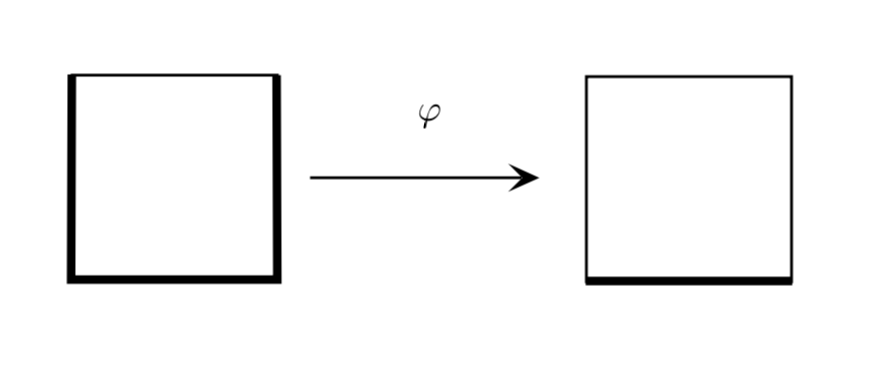
\includegraphics[scale=0.5]{varp}
\end{center}
Thus the diagram 
$$
\begin{tikzcd}
E_{b_0}\times I\times\{0\} \arrow[d, hook] & E_{b_0}\times U \arrow[r, "\Gamma"] \arrow[d, hook] \arrow[l, "id\times \varphi"'] & E \arrow[d, "p"] \\
E_{b_0}\times I\times I \arrow[rru, "\Lambda'", dashed] & E_{b_0}\times I\times I \arrow[r, "\Lambda"'] \arrow[l, "id\times \varphi"] \arrow[ru, "\tilde{\Lambda}", dashed] & B
\end{tikzcd}
$$
has the left two horizontal maps homeomorphisms. Since the homotopy applies to the outside square, there exists a lift $\tilde{\Lambda}:=\Lambda'\circ id\times\varphi$. Thus defined $\tilde{\Lambda}$ is a lift of $\Lambda$ and commutes with the right square.

Therefore we have
$$
\tilde{\Lambda}(e,s,0)=\Gamma(e,s,0)=\tilde{H}(e,s)
$$
$$
\tilde{\Lambda}(e,s,1)=\Gamma(e,s,1)=\tilde{H}'(e,s)
$$

This gives a homotopy from $\tilde{H}$ to $\tilde{H}'$. Restricting to $E_{b_0}\times \{1\}$ we obtain a homotopy from $\tilde{H}_1$ to $\tilde{H}'_1$. Thus the homotopy class $\alpha_*=[\tilde{H}_1]$ depends only on the homotopy class of $\alpha$ relative to end points, establishing the claim. 

Clearly $(\alpha\beta)_*=\beta_*\circ \alpha_*$ if $\beta(0)=\alpha(1)$. In particular, if $\beta=\alpha^{-1}$ then $(const)_*=\beta_*\circ \alpha_*$, where const denote the constant path at $b_0$. But clearly, $(const)_*=[id_{E_{b_0}}]$, therefore $\alpha_*$ is a homotopy equivalence, and since $B$ is path connected, all fibers are homotopy equivalent.

The following exercise completes the proof.
\end{proof}
\begin{exr}
Show that the set of homotopy classes of self-homotopy equivalence of a space $X$ forms a group under composition.
\end{exr}
\begin{proof}
Assume $h_1,h_2: X\lrta X$ are homotopy equivalence from $X$ to $X$ itself. And we denote by $[h_1],[h_2]$ the homotopy classes of them. An obvious choice of multiplication is
$$
[h_1]*[h_2]:=[h_1\circ h_2]
$$
This map is well-defined because composition of homotopic maps are homotopic.
$[id_X]$ is an identity in this group. By definition of homotopy equivalence. Assume $g$ is one homotopy inverse of $h$, we have $gh\simeq id_X$ and $hg\simeq id_X$, therefore, $[g]*[h]=[id_X]$ and $[h]*[g]=[id_X]$.
\end{proof}
\begin{definition}
With a little bit abuse of terminology, we refer to any space in the homotopy class of the space $E_b$ for any $b\in B$ as the fiber of the fibration $p: E\lrta B$.
\end{definition}

Since homotopy equivalences induces isomorphism in homology or cohomology, a fibration with fiber $F$ gives rise to local coefficients systems whose fiber is the homology or cohomology of $F$, as the next corollary asserts.

\begin{corollary}

\end{corollary}
\chapter{Homotopy groups}
\chapter{Stable homotopy. Daulity}
\chapter{Cell complexes}
%----------------------------------------------------------------------------------------
%	CHAPTER 1
%----------------------------------------------------------------------------------------


%---------------------------------------------------------------------------------------

%\part{Homologies}

\chapter{Singular homology}
\section{Singular Homology Groups}
\section{The Fundamental Group
}

\section{Homotopy
}
\section{Barycentric Subdivision. Excision}
\section{Weak Equivalences and Homology}
\section{Homology with Coefficients}
\section{The Theorem of Eilenberg and Zilber}
\section{The Homology Product}
\chapter{Homology}
\section{The Axioms of Eilenberg and Steenrod}


\chapter{Homological algebra}
\section{Diagrams}
\section{Exact sequences}
\section{Chain complex}
\section{Cochain complex}
\section{Natural chain maps and homotopies}
\section{Linear algebra of chain complexes}
\begin{definition}
Suppose $(C_\bullet,\pd)$ and $(C'_\bullet,\pd')$ are two non-negative chain complexes. We define the  \textbf{tensor complex} $(C_\bullet\otimes C_\bullet',\Delta)$, where
$$
(C_\bullet\otimes C'_\bullet)_n=\oplus_{i+j=n}C_i\otimes C_j'
$$
and the differential $\Delta$ is defined by 
$$
\Delta(c_i\otimes c'_j)=\pd c_i\otimes c'_j+(-1)^{i}c_i\otimes \pd' c_j
$$
\end{definition}
\begin{definition}
Suppose $f_\bullet:C_\bullet\lrta D_\bullet$ and $g_\bullet: C'_\bullet\lrta D'_\bullet$ are two morphism of chain complexes. Then we can define a chain map
$$
f\otimes g: C_\bullet\otimes C_\bullet'\lrta D_\bullet\otimes D_\bullet'
$$
by 
$$
(f\otimes g)_n=\sum_{i+j=n}f_i\otimes g_j
$$
It is easy to check this is indeed a chain map.
\end{definition}
\begin{exr}
Tensor product is compatible with chain homotopy. Let $s:  f \simeq g: C_\bullet\lrta C_\bullet'$  be a chain homotopy. Then $s\otimes id :f\otimes id  \simeq g \otimes id : C_\bullet\otimes D_\bullet \lrta C_\bullet' \otimes D_\bullet$ is a chain homotopy.
\end{exr}
\begin{proof}
\underline{Know}: $ s\pd_{C}+\pd_{C'} s=f-g$

\underline{Want}: $(s\otimes id_D)\pd_{C\otimes D} +\pd_{C'\otimes D} (s\otimes id_D)=f\otimes id_D-g\otimes id_D$. 

$C\otimes D$ is generated by pure tensors like $c'_n\otimes d_m$, therefore we can  check the formula on element $c_n\otimes d_m\in C_n\otimes D_m$
$$
\begin{aligned}
&(s\otimes id_D)\pd_{C\otimes D}(c_n\otimes d_m)\\
&=(s\otimes id_D)\left(\pd_C c_n\otimes d_m +(-1)^n c_n\otimes\pd_D d_m\right)\\
&=s\circ \pd_C c_n\otimes d_m+(-1)^n s c_n\otimes \pd_D d_m
\end{aligned}
$$
and
$$
\begin{aligned}
&\pd_{C'\otimes D} (s\otimes id_D)(c_n\otimes d_m)\\
&=\pd_{C'\otimes D} (s c_n\otimes d_m)\\
&= \pd_{C'} s c_n \otimes d_m+(-1)^{\deg(sc_n)}sc_n\otimes \pd_D d_m,
\end{aligned}
$$
where $\deg (sc_n)=n-1$. Then we have
$$
\begin{aligned}
&\left(\pd_{C'\otimes D} (s\otimes id_D)+(s\otimes id_D)\pd_{C\otimes D}\right) (c_n\otimes d_m)\\
&=(s\pd_C+\pd_{C'} s)c_n \otimes d_m+0\\
&=(f\otimes id_D-g\otimes id_D)(c_n\otimes d_m)
\end{aligned}
$$
We are done. Also we can generalize this statement to 

 Let $s:  f \simeq g: C\lrta C'$ and  $t:  p \simeq q: D\lrta D'$ be chain homotopies. Then $s\otimes t :f\otimes p  \simeq g \otimes q : C\otimes D \lrta C' \otimes D'$ is a chain homotopy. We easily conclude by $s\otimes id$ and $id\otimes t$ are chain homotopy and composition of chain homotopies is a chain homotopy.
\end{proof}

\begin{exr}\label{chap11exr:free_acyclic_contracting_chain_homotopy}
Let $(C_\bullet,\pd)$ be a free chain complex. Then $C_\bullet$ is acyclic iff it  has contracting chain homotopy
\end{exr}
\begin{proof}
A contracting homotopy means $Q:C_n\lrta C_{n+1}$ s.t. $Q\pd+\pd Q=id$. 

If such $Q$ exists then $H_n(C_\bullet)=0\forall n$. That direction doesn't require $C_\bullet$ to be free.

As for the reverse direction, consider
$$
B_n\subseteq Z_n\subseteq C_n
$$
If we assume $C_\bullet$ is acyclic then
$$
B_n=Z_n,\forall n
$$ 
$$
0\lrta Z_n \overset{i}{\lrta} C_n\overset{\pd}{\lrta}Z_{n-1}\lrta 0
$$

Since $Z_{n-1}$ is free abelian  the sequence splits $\exists r_n:Z_{n-1}\lrta C_n$ s.t. $\pd\circ r_n=id$. Note that $id- r_{n-1}\circ \pd$ has image in $Z_{n-1}$, $c\in C_n$. $\pd(c-r_n\pd c)=\pd c-\pd c=0$

Now define 
$Q_n:C_n\lrta C_{n+1}$ by $Q_{n}=r_n (id-r_{n-1}\circ\pd)$. This works.
$$
\begin{aligned}
\pd Q_n +Q_{n-1}\pd
&=\pd r_n (id -r_{n-1}\pd)+r_{n-1}( id-r_{n-2}\pd )\pd\\
&=id -r_{n-1}\pd+r_{n-1}\pd -r_{n-1}r_{n-2}\pd^2\\
&=id
\end{aligned}
$$
\end{proof}
\begin{definition}
Suppose $f:(C_\bullet,\pd)\lrta (D_\bullet,\pd')$. The \textbf{mapping cone } of $f$ is the chain complex $Cone_\bullet(f),\pd^f$, where $Cone_n(f)=C_{n-1}\otimes D_n$ and 
$\pd^f:Cone_n(f)\lrta Cone_{n-1}(f)$
$$
\pd^f(c,d)=(-\pd c,f c+\pd' d)
$$
$$
\pd^f=
\begin{pmatrix}
&-\pd & 0\\
& f &\pd'
\end{pmatrix}
$$
\end{definition}
\begin{exr}\label{chap11exr:acyclic_mapping_cone_chain_equivalence}
If $f:C_\bullet\lrta D_\bullet$ is a chain map between two free chain complexes and $Cone_\bullet(f)$ is acyclic then prove $f$ is  a chain equivalence.
\end{exr}
\begin{proof}
Note that the definition of mapping cone implies $Cone_\bullet(f)$ to be a free chain complex. Then we can apply Exercise~\ref{chap11exr:free_acyclic_contracting_chain_homotopy} and there is a contracting chain homotopy
$Q$ such that $$
Q\pd^f+\pd^f Q=id
$$
$$
Q=
\begin{pmatrix}
p & g\\
r & -p'
\end{pmatrix}
$$
$$
\begin{pmatrix}
\pd & 0\\
f & -\pd'
\end{pmatrix}
\begin{pmatrix}
p & g\\
r & -p'
\end{pmatrix}
+
\begin{pmatrix}
p & g\\
r & -p'
\end{pmatrix}
\begin{pmatrix}
\pd & 0\\
f & -\pd'
\end{pmatrix}
=\begin{pmatrix}
id & 0\\
0 & id
\end{pmatrix}
$$
$$
\begin{pmatrix}
-\pd p-p\pd +gf & -\pd g+g \pd'\\
* & fg-\pd' p'-p'\pd'
\end{pmatrix}=
\begin{pmatrix}
id & 0\\
0 & id
\end{pmatrix}
$$
Then we know 
$g:D_\bullet \lrta D_\bullet$ is a chain map

$p\pd +\pd p=gf-id$

$p'\pd'+\pd'p'=fg-id$. Thus $f$ is a chain equivalence with inverse $g$.
\end{proof}
\begin{lemma}
Let $f: C_\bullet\lrta D_\bullet$. Then there is a LES
$$
\cdots\lrta H_{n+1}(Cone_\bullet(f))\lrta H_n(C_\bullet)\overset{H_{n}(f)}{\lrta} H_n (D_\bullet)\lrta H_n(Cone_\bullet(f))\lrta \cdots
$$
\end{lemma}
\begin{proof}
Denote by $C^+_\bullet$ the chain complex $C^+_n=C_{n-1}$. There is a SES
$$
0\lrta D_\bullet\overset{i}{\lrta} Cone_\bullet(f)\overset{p}{\lrta} C^+_\bullet\lrta 0
$$
with $i(d)=(0,d)$ and $p (c,d)=c$

Pass to the LES in homology
\[
\begin{tikzcd}
\cdots  \arrow[r] & H_{n+1}(Cone_\bullet(f)) \arrow[r] & H_{n+1}(C^+_\bullet) \arrow[r,"\delta"] \arrow[d, equal] & H_n(D_\bullet) \arrow[r] & H_n(Cone_\bullet(f)) \arrow[r] & \cdots \\
 &  & H_n(C_\bullet) &  &  & 
\end{tikzcd}
\]

It remains to check $\delta=H_n(f)$.


Note if $c$ is a cycle in $C_n$. Then 
$$
\pd^f\circ p^{-1}(c)=(-\pd c, fc)=(0,fc)=i(fc)
$$
$$
\delta:\lgl c\rgl\longmapsto \lgl i^{-1}\pd^fp^{-1}c\rgl=\lgl fc\rgl= H_{n}(f)\lgl c\rgl
$$
\end{proof}
\begin{exr}\label{chap11exr:free_chain_equivalence_isomorphic_homology}
Suppose $f:C_\bullet\lrta D_\bullet$ is  a chain map between the two free chain complex . Then $f$ is a chain equivalence iff 
$$
H_n(f): H_n(C_\bullet)\lrta H_n(D_\bullet)
$$
is an isomorphism for all $n$,
\end{exr}
\begin{proof}
If $f$ is a chain equivalence then $H_n (f)$ is always a isomorphism. This does not require any freeness assumptions and we proved in last semester.

For the converse, if $H_n(f)$ is always an isomorphism, then the LES
$$
\cdots\lrta H_{n+1}(Cone_\bullet(f))\lrta H_n(C_\bullet)\overset{\cong}{\lrta} H_n (D_\bullet)\lrta H_n(Cone_\bullet(f))\lrta \cdots
$$
This implies $H_n(Cone_\bullet (f))=0,\forall n$. Then $Cone_\bullet(f)$ is acyclic, and we can conclude by Exercise~\ref{chap11exr:acyclic_mapping_cone_chain_equivalence}.
\end{proof}
\section{Tor and Ext}
\begin{definition}
Suppose $A$ is an abelian group, A \textbf{Free resolution} is an exact sequence of the form
$$
\cdots\lrta F_2\overset{f_2}{\lrta}F_1\overset{f_1}{\lrta}F_0\overset{f_0}{\lrta}A\lrta 0,
$$
where each $F_i$ is a free abelian group. If moreover $F_i=0,\forall i\geq 2$, we call it \textbf{Short free resolution} 
$$
0\lrta K\lrta F\lrta A\lrta 0
$$
\end{definition}
(We can easily generalize this definition to $R$-modules)
\begin{proposition}
Let $A$ be an abelian group. Then there exists a short free resolution of $A$.
\end{proposition}
\begin{proof}
Let $F$ be the free abelian group generated by all elements in $A$. There is a surjection from $F$ to $A$ by linearly extending the map sending basis element to itself. Let $K$ denote the kernel of this map. $K$ is an abelian subgroup of a free abelian group ($\intg$-module).  A subgroup of a free abelian group is torsion free as a module. $\intg$ is a $PID$. If $R$ is a $PID$, then an  $R$-module is free iff it is torsion free (See Bosch section 4.2). Then we know in particular, $K$ is a free abelian group.
\end{proof}
With this construction, we can define the $\tor$ functor now:
\begin{definition}
Let $A$ be an abelian group. Let $0\rta K\overset{f}{\rta}F\rta A\rta 0$ be a short free resolution of $A$. Given any other abelian group $B$ and apply the functor $\otimes B$ to it. We get an exact sequence
$$
K\otimes B\overset{f\otimes id_B}{\lrta} F\otimes B\lrta A\otimes B\lrta 0
$$
We define 
$$
\tor(A,B):=\ker(f\otimes id_B).
$$
It measure the failure of $\otimes B$ to be left exact.
\tor(A,B) can be more generally defined in the category of $R$-modules, where $R$ is a principal ideal ring, where short free resolution does exist. 
\end{definition}

\begin{exr}\label{chap11exr:tor_functor}
Given $h: A\lrta A'$ a homomorphism of abelian group define the induced morphism
$$
\tor(h, B): \tor (A,B)\lrta \tor(A',B).
$$ 
Use this argument to show that $\tor(A, B)$ is well-defined (independent on the choice of short free resolutions)
\end{exr}
\begin{proof}
Let $0\lrta K\lrta F\lrta A\lrta 0$ and $0\lrta K'\lrta F'\lrta A'\lrta 0$ be two short free resolutions of $A$ and $A'$ respectively, and denote by $C_\bullet$ and $C'_\bullet$ the corresponding chain complexes. 
$$
C_n=\left\{ \begin{aligned}
F, & n=0\\
K, & n=1\\
0, & n\neq 0,1
\end{aligned}
\right.
$$
with the only nontrivial boundary map $\pd: C_1\lrta C_0$ to be $f: K\lrta F$ and $C_\bullet'$ is defined similarly. We have $H_0(C_\bullet)=A$ and $H_0(C_\bullet')=A'$. We can therefore think of $h: A\lrta A'$ as a homomorphism $H_0(C_\bullet)\lrta H_0(C_\bullet')$. Now we can invoke Corollary~\ref{appendixAcor:chain_homotopy_over_H0(f)_free_acyclic}, which tells us there exists a chain map $g_\bullet: C_\bullet\lrta C_\bullet'$ with $H_0(g_\bullet)=h$. 

Tensoring with $B$, we get a chain map $g_\bullet\otimes id_B:C_\bullet\otimes B\lrta C_\bullet'\otimes B$ because $\otimes B$ is a functor. Now pass to the first homology group to get a map
$$
H_1(g_\bullet\otimes id_B): H_1(C_\bullet\otimes B)\lrta H_1(C_\bullet'\otimes B).
$$
However, by definition $H_1(C_\bullet\otimes B)=\tor(A,B)$, we therefore have defined the morphism induced by $\tor(\square,B)$
$$
\tor(h,B):H_1(g_\bullet\otimes id_B)
$$

In order to prove $\tor(A,B)$ is well-defined, we consider the case where $A=A'$, again still by~\ref{appendixAcor:chain_homotopy_over_H0(f)_free_acyclic}, we obtain a chain map $g_\bullet: C_\bullet\lrta C_\bullet'$ with $H_0(g_\bullet)=id_A$ and this chain map $g_\bullet: C_\bullet\lrta C_\bullet$ is a chain equivalence thus induces chain equivalence $g_\bullet\otimes id_B$ and finally we have 
$$
H_1(C_\bullet\otimes B)=H_1(C'_\bullet\otimes B).
$$
Therefore two different short free resolution determines identical $\tor(A,B)$.
\end{proof}
\begin{remark}
The above exercise means basically for each fixed abelian group $B$, $\tor(\square, B):Ab\lrta Ab$ is a covariant functor. In a similar vein, we can also fix the first variable of $\tor$ and define $\tor(A,\square): Ab\lrta Ab$ as a covariant functor. 
\end{remark}
\begin{exr}
Define $\tor(A,h)$ for a given homomorphism $h: B\lrta B'$.
\end{exr}
\begin{proof}
This case is easier, the homomorphism $h: B\lrta B'$ induces a morphism of chain complexes $id_{C_\bullet}\otimes h$ and thus induces the morphism $\tor(A,h):=H_1(id_{C_\bullet}\otimes h):\tor(A,B)\lrta \tor(A,B')$
\end{proof}
\begin{theorem}
(Properties of $\tor$)
\begin{enumerate}[label=(\arabic*)]
\item If either $A$ or $B$ are torsion-free abelian groups then $\tor(A,B)=0$
\item If $T(A)$ denotes the torsion subgroup of $A$ then for any abelian group $B$, one has 
$$
\tor(A,B)\cong \tor(T(A),B).
$$
\item 
If $0\lrta B\lrta B'\lrta B''\lrta 0$ is exact, then for any $A$, there is an exact sequence
$$
\begin{tikzcd}
0 \arrow[r] & \tor(A,B) \arrow[r] & \tor(A,B') \arrow[r] & \tor(A,B'') \arrow[lld] &  \\
 & A\otimes B \arrow[r] & A\otimes B' \arrow[r] & A\otimes B'' \arrow[r] & 0
\end{tikzcd}
$$

If $0\lrta A\lrta A'\lrta A''\lrta 0$ is a short exact sequence, then for any abelian group $B$, there is an exact sequence
$$
\begin{tikzcd}
0 \arrow[r] & \tor(A,B) \arrow[r] & \tor(A',B) \arrow[r] & \tor(A'',B) \arrow[lld] &  \\
 & A\otimes B \arrow[r] & A'\otimes B \arrow[r] & A''\otimes B \arrow[r] & 0
\end{tikzcd}
$$
\item For any two abelian groups $A,B$, $\tor(A,B)\cong \tor(B, A)$.
\item If $B$ is an abelian group and $\{A_\lambda|\lambda\in \Lambda\}$ is a (possibly uncountable ) family of abelian groups then there is an isomorphism
$$
\tor\left(\bigoplus_{\lambda\in\Lambda}A_\lambda, B\right)\cong \bigoplus_{\lambda\in\Lambda}\tor(A_\lambda, B)
$$
and 
$$
\tor\left(B,\bigoplus_{\lambda\in \Lambda}A_\lambda\right)\cong\bigoplus \tor(B,A_\lambda).
$$
\item For any $m\in \mathbb{N}$ and any abelian group $B$,
$$
\tor(\intg/m\intg, B)\cong \{b\in B| mb=0\}
$$
\end{enumerate}
\end{theorem}
\begin{proof}
$(1)$ A torsion free abelian group $B$ is a free $\intg$-module, $\otimes B$ is there fore exact functor, in this case we have $\tor(A,B)=0$ for all $A$. 

On the other hand, if $A$ is free, we can choose a silly short free resolution: $0\lrta 0\lrta A\lrta A\lrta 0$. Then clearly, $\tor(A,B)=0$ for any $B$. We have not prove the case where $A$ is merely torsion free, it will follows directly from $(4)$ and the case $B$ is torsion free. 

Then we skip part $(2)$ and prove the first statement of  $(3)$.
Given an exact sequence $0\lrta B\lrta B'\lrta B''\lrta 0$. let $0\lrta K\lrta F\lrta A\lrta 0$ be short free resolution. Then we know $K\otimes \square$ and $F\otimes \square$ are exact functors. We have a commutative diagram
$$
\begin{tikzcd}
0 \arrow[r] & K\otimes B \arrow[r] \arrow[d] & K\otimes B' \arrow[r] \arrow[d] & K\otimes B'' \arrow[r] \arrow[d] & 0 \\
0 \arrow[r] & F\otimes B \arrow[r] & F\otimes B' \arrow[r] & F\otimes B'' \arrow[r] & 0
\end{tikzcd}
$$
This means we have a short exact sequence of chain complexes
$$
0\lrta C_\bullet\otimes B\lrta C_\bullet\otimes B'\lrta C_\bullet\otimes B''\lrta 0.
$$
It induces a long exact sequence in homology which is just the desired six-term exact sequence in $(3)$. 

The second statement would follow directly from $(4)$ and the first statement of $(3)$.

Then we prove part $(4)$. Given a short free resolution $0\lrta K\lrta F\lrta A\lrta 0$. Because $K,F$ are free, we know $\tor(B,K)=0$ and $\tor(B,F)=0$ from what we have proved in $(1)$. (there is no circular deduction).  Then, from the first statement of $(3)$, we obtain an exact sequence
$$
0\lrta 0\lrta 0\lrta \tor(B,A)\lrta B\otimes K\lrta B\otimes F\lrta B\otimes A\lrta 0.
$$
Also from the definition of $\tor(A,B)$ the bottom row of the next  diagram is exact.
$$
\begin{tikzcd}
0 \arrow[r] & 0 \arrow[d, "\cong"] \arrow[r] & \tor(B,A) \arrow[d] \arrow[r] & B\otimes K \arrow[d, "\cong"] \arrow[r] & B\otimes F \arrow[d, "\cong"] \arrow[r] & B\otimes A \arrow[d, "\cong"] \arrow[r] & 0 \\
0 \arrow[r] & 0 \arrow[r] & \tor(A,B) \arrow[r] & K\otimes B \arrow[r] & F\otimes B \arrow[r] & A\otimes B \arrow[r] & 0
\end{tikzcd}
$$
Then we know from five lemma that $\tor(B,A)\cong \tor(A,B)$

Up to now, we have totally proved $(1)$ and $(3)$ and we come to $(2)$. For any abelian group, if $T(A)$ denote the torsion subgroup, $A/T(A)$ is torsion free. We therefore have $\tor(A/T(A), B)=0$ for any abelian group from $(1)$. Then we apply the second statement of $(3)$  to the short exact sequence $0\lrta T(A)\lrta A\lrta A/T(A)\lrta 0$ and first three terms of the six-term exact sequence is
$$
0\lrta \tor(T(A),B)\lrta\tor(A,B)\lrta 0.
$$

For each $A_\lambda$, we can find a short free resolution $0\lrta K_\lambda\lrta F_\lambda\lrta A_\lambda\lrta 0$ and 
$$
0\lrta \oplus_\lambda K_\lambda\lrta \oplus_\lambda F_\lambda\lrta \oplus_\lambda A_\lambda\lrta 0
$$ is a free resolution of $\oplus_\lambda A_\lambda$. Then
$$
\tor(\oplus_{\lambda\in \Lambda} A_\lambda, B)=\ker\left(\oplus_\lambda K_\lambda\otimes B\lrta \oplus_\lambda F_\lambda\otimes B\right)=\bigoplus_\lambda\ker\left(K\otimes B\lrta F\otimes B\right).
$$
This prove the first statement of $(5)$ and we can prove the second combined with $(4)$.

(6), we can consider the short free resolution $0\lrta \intg\overset{m}{\lrta}\intg\lrta \intg/m\intg\lrta 0$ 
$$
\tor(\intg/m\intg, B)=\ker(B\overset{m}{\lrta} B)
$$

\end{proof}

\begin{definition}
Suppose $A$ is an abelian group and let 
$
0\lrta K \overset{f}{\lrta} F\lrta A\lrta 0
$
be a short free resolution. Take another abelian group $B$ and apply $\hom(\square, B)$, we can find an exact sequence
$$
0\lrta \hom(A, B)\lrta \hom(F,B) \overset{\hom(f,B)}{\lrta} \hom(K,B)
$$
and we define $\ext(A,B):=\coker\hom(f,B)=\hom (K,B)/\im \hom(f,B)$. Thus $\ext (A,B) $ measures the failure for $\hom(\square, B)$ to be right exact.
\end{definition}
Here is a more sophisticated way of viewing $\ext (A,B)$ consider a chain complex $C_1=K$, $C_0=F$, $\pd_1:C_1\lrta C_0=f: K\lrta F$ and all other group zero. $H_0(C_\bullet)=A$. Now apply $\hom(\square, B)$ to a cochain complex $\hom(C_\bullet ,B)$, the definition of $\ext (A,B)$ gives us immediately that
$$
H^1(\hom(C_\bullet,B))=\ext(A,B).
$$
From this it follows that $\ext(\square, B)$ is a contravariant functor and it is well defined (independent of the choice of short free resolution.)
\begin{definition}
An abelian group $D$ is said to be \textbf{divisible} if  for every $b\in D$ and every $n\in \mathbb{N}$ there exists an $a\in D$ s.t., $na=b$
\end{definition}

\begin{theorem}
(Properties of $\ext$)

For a fixed abelian group $A$, $\ext(\square, A)$ is a contravariant functor and $\ext(A,\square)$ is a covariant functor. Moreover,
\begin{enumerate}[label=(\arabic*)]
\item If $A$ is a free group, then $\ext (A,B)=0,\forall B$. If $D$ is a divisible abelian group, then $\ext (A,D)=0\forall A$.
\item If  $A$ is a finitely generated group with torsion subgroup $T(A)$ then $\ext(A,\intg)=T(A)$
\item $0\lrta A\lrta A'\lrta A''\lrta 0$ is exact, then for any $B$, there is an exact sequence
$$
\begin{tikzcd}
0 \arrow[r] & \hom(A'',B) \arrow[r] & \hom(A',B) \arrow[r] & \hom(A,B) \arrow[lld] &  \\
 & \ext(A'',B) \arrow[r] & \ext(A',B) \arrow[r] & \ext(A,B) \arrow[r] & 0
\end{tikzcd}
$$


If $0\lrta B\lrta B'\lrta B''\lrta 0$ is exact, then for any $A$, there is an exact sequence
$$
\begin{tikzcd}
0 \arrow[r] & \hom(A,B) \arrow[r] & \hom(A,B') \arrow[r] & \hom(A,B'') \arrow[lld] &  \\
 & \ext(A,B) \arrow[r] & \ext(A,B') \arrow[r] & \ext(A,B'') \arrow[r] & 0
\end{tikzcd}
$$
\item If $B$ is an abelian group and $\{A_\lambda|\lambda\in \Lambda\}$ is a collection of abelian group then 
$$
\ext\left(\bigoplus_{\lambda\in\Lambda} A_\lambda,B\right)\cong \prod_{\lambda\in \Lambda} \ext(A_\lambda, B)
$$
$$
\ext\left(B, \bigoplus_{\lambda\in \Lambda} A_\lambda\right)\cong \prod_{\lambda\in \Lambda} \ext(B,A_\lambda)
$$
\item For any $m\in \mathbb{N}$ and any $B$
$$
\ext(\intg/ m\intg, B)\cong B/mB
$$
\end{enumerate}
\end{theorem}
\begin{proof}
 $\ext(A,\square)$ and $\ext(\square, A)$ are covariant functor and contravariant functor respectively. The proof is identical to those in~\ref{chap11exr:tor_functor}.

 $(3)-(5)$ can be proved similar to those proof for $\tor$ although we have $\ext(A, B)\neq \ext B,A$ in general.

For the first six-term exact sequence, we can
need an auxiliary fact
$$
\tiny
\begin{tikzcd}
 & 0 & 0 & 0 &  \\
0 \arrow[r] & A \arrow[r, "f"] \arrow[u] & A' \arrow[r, "g"] \arrow[u] & A'' \arrow[r] \arrow[u] & 0 \\
0 \arrow[r] & F \arrow[r, "i_1"] \arrow[u, "u"] & F\oplus F'' \arrow[r, "p_1"] \arrow[u, "u'", dashed] & F'' \arrow[r] \arrow[u, "u''"] & 0 \\
0 \arrow[r] & K \arrow[r, "i_2"] \arrow[u, "v"] & K\oplus K'' \arrow[r, "p_2"] \arrow[u, "v'", dashed] & K'' \arrow[r] \arrow[u, "v''"] & 0 \\
 & 0 \arrow[u] & 0 \arrow[u] & 0 \arrow[u] & 
\end{tikzcd}
$$
Given the first and third column to be short free resolutions and the first row exact, we can construct the middle column to be a short free resolution of $A'$ and each row is exact.

This is guaranteed by the \href{https://en.wikipedia.org/wiki/Horseshoe_lemma}{Horseshoe lemma}

 For the second six-term exact sequence we consider
 $0\lrta K\overset{f}{\lrta} F\lrta 0$ is a chain complex of free abelian group. Free module is a special case of projective module, hence $\hom(K,\square)$ and $\hom(F,\square)$ are exact functors. 

 Then we have the 
 short exact sequence of chain complexes
 $$
0\lrta C_\bullet\lrta C'_\bullet\lrta C''_\bullet\lrta 0.
 $$
 Because each row splits, we also have the SES of  cochain complexes
 $$
0\lrta \hom(C''_\bullet,B)\lrta\hom(C'_\bullet, B)\lrta \hom(C_\bullet, B)\lrta 0
 $$
 and we derive the six-term LES from it.

$$
\begin{tikzcd}
0 \arrow[r] & \hom(K, B) \arrow[r] \arrow[d] & \hom(K, B') \arrow[r] \arrow[d] & \hom(K, B'') \arrow[r] \arrow[d] & 0 \\
0 \arrow[r] & \hom(F, B) \arrow[r] & \hom(F, B') \arrow[r] & \hom(F, B'') \arrow[r] & 0
\end{tikzcd}
$$
which is a short exact sequence of cochain complexes
$$
0\lrta \hom(C_\bullet, B)\lrta \hom(C_\bullet, B')\lrta \hom(C_\bullet, B'')\lrta 0
$$

 (1) If $A$ is a free abelian group, then the free resolution $0\lrta K\lrta F\lrta A\lrta 0$ splits then when applied with functor $\hom(\square, B)$, we still get an exact sequence
 $$
0\lrta \hom(A, B)\lrta \hom(A\oplus K,B) \overset{\hom(f,B)}{\lrta} \hom(K,B)\lrta 0
$$
 whatever $B$ is. $\hom(f,B)(\varphi)=\varphi\circ f$, it is now surjective because for any $v\in \hom(K,B)$, we can choose $0\oplus v\in\hom(A\oplus K, B)$ so that $(0\oplus v)\circ f=v$.

 For the second statement, we \underline{Claim}: when $D$ is divisible, $\hom(\square, D)$ is exact.

 It suffices to prove $\hom(f, D)$ is surjective
$$
0\lrta \hom(A, D)\lrta \hom(F,D) \overset{\hom(f,D)}{\lrta} \hom(K,D)\lrta 0
$$
\end{proof}

\section{Universal coefficients}
\section{Algebraic K\"unneth formula}
In this section
we would prove an algebraic version of K\"unneth formula for free chain complexes. In the next section we would prove Eilenber-Zilber theorem and then derive the general K\"unneth formula as a corollary of the algebraic one. 
\begin{theorem}\label{chap11thm:Algebraic_Kuenneth_formula}
(Algebraic K\"unneth Theorem) Let $(C,\pd)$ and $(D,\pd')$ be two non-negative free complex. Then for every $n\geq 0$, there is a split exact sequence
$$
0\lrta \oplus_{i+j=n}H_i(C_\bullet)\otimes H_j(D_\bullet)\overset{\omega}{\lrta} H_n(C_\bullet\otimes D_\bullet)\lrta \oplus_{k+\ell=n-1}\tor(H_k(C_\bullet),H_\ell(D_\bullet))\lrta 0
$$
where $\omega$ is the map $\langle c_i\rangle\otimes \lgl d_j\rgl\mapsto \lgl c_i\otimes d_j\rgl$. 
Thus there also exists a (non-natural) isomorphism 
$$
H_n(C_\bullet\otimes D_\bullet)\cong \left(\bigoplus_{i+j=n}H_i(C_\bullet)\otimes H_j (D_\bullet)\right)\oplus\left(\bigoplus_{k+\ell=n-1} \tor(H_k(C_\bullet),H_\ell(D_\bullet))\right)
$$
\end{theorem}
\section{Eilenberg-Zilber theorem and K\"unneth formula}
\begin{theorem}
(Eilenberg-Zilber) if $X$ and $Y$ are two topological spaces. There is a nontrivial chain equivalence
$$
\Omega_\bullet: C_\bullet(X\times Y)\lrta C_\bullet(X)\otimes C_\bullet (Y)
$$

which is unique up to chain homotopy.
\end{theorem}
\begin{proof}
$Top\times Top$ is the category of pairs $(X,Y)$ of topological spaces.

We will define two functor from $Top\times Top\lrta Comp$
$$S_\bullet(X,Y)=C_\bullet(X,Y),\ \  T_\bullet (X,Y)=C_\bullet(X)\otimes C_\bullet(Y)$$

For models
$$
\pzm=\{(\Delta^i,\Delta^j), i,j \geq 0\}
$$ 
\underline{Claim}: $S_\bullet$ and $T_\bullet$ are both acyclic in positive degree on $\pzm$ and free with basis contained in $\pzm$

$S_\bullet$, $H_n(S_\bullet(\Delta^i, \Delta^j))=H_n(\Delta^i\times \Delta^j)=0$, $\forall n>0, \forall i,j$ (Acyclic in positive degrees)

$S_i: Top\times Top\lrta Ab$

$S_i(X, Y)=C_i (X\times Y)$\\
\underline{subclaim}: $\{(\Delta^i,\Delta^i)\}$ is a $S_i$-model set and the diagonal map $d_i:\Delta^i\lrta\Delta^i\otimes \Delta^i$  $x\mapsto (x,x)$ gives a model basis.

Indeed, if $(X,Y)$ is any object in $Top\times Top$ and if $
\sigma: \Delta^i\lrta X\times Y
$ is any singular simplex in $S_i(X\times Y)=C_i(X\times Y)$, then we can write 
$\sigma=(\sigma_x,\sigma_y)\circ d_i$,  where $\sigma_x=p_X\circ \sigma$ be the composition of $\sigma$ with $p_X:X\times Y\lrta X$.
$S_i(\tau)(d_i), \tau\in \hom(\Delta^i\times \Delta^i,X\times Y)$ forms a basis of the free abelian group $S_i(X\times Y)=C_i(X\times Y)$.

As for $T_i$, we quote the exercise, for any $(X,Y)\in Top\times Top$, $C_i(X)\otimes C_j(Y)$ is free abelian with ba

 $T_i(X\times Y)=(C_\bullet(X)\otimes C_\bullet(Y))$. $T_i(X, Y)$ is the tensor product of the free groups and thus is free.
$\{(\ell_i,\ell_j)|i+j=n\}$ is a $T_n$-model basis.

The last thing to check is that $T_\bullet(\Delta^i, \Delta^j)$ is acyclic in positive degrees
$$
H_n(C_\bullet(\Delta^i)\otimes C_\bullet(\Delta^j))=0,\forall n>0.
$$
We can not compute this! However we can cheat
$$
H_n(C_\bullet(\Delta^i))=H_n(\Delta^i)=\left\{\begin{matrix}
 \intg & n=0\\
 0 & n\neq 0
\end{matrix}\right.
$$

Consider the chain complex
$$
0\lrta 0\lrta \cdots\lrta 0\lrta \intg\lrta 0\cdots
$$
$C_\bullet(\Delta^i)$ has the same homology as this complex. Thus $C_\bullet(\Delta^i)$ is equivalent to the complex and $C_\bullet(\Delta^j)$ is also chain equivalent to it (By Exercise~\ref{chap11exr:free_chain_equivalence_isomorphic_homology}). $C_\bullet(\Delta^i)\otimes C_\bullet(\Delta^j)$ is chain equivalent to 
$$
0\lrta 0\lrta \cdots\lrta 0\lrta \intg\otimes \intg\lrta 0\cdots
$$
Thus $H_n(C_\bullet(\Delta^i)\otimes C_\bullet(\Delta^j))=H_n(\cdots\lrta0\lrta \intg\otimes \intg\lrta 0\cdots)$. We then know $T_\bullet(\Delta^i,\Delta^j)$ is indeed acyclic in positive degrees. 

We have now verified that the hypotheses of the Acyclic Models Theorem and
its corollary are satisfied.
Define  
$\Theta:H_0\circ S_\bullet\lrta H_0\circ T_\bullet$ is a natural equivalence.
$$
\Theta(X\times Y):H_0(C_\bullet(X\times Y))\lrta H_0(C_\bullet(X)\otimes C_\bullet (Y))
$$
$$
\lgl c_{(x,y)}\rgl\mapsto \lgl c_x\rgl\otimes\lgl c_y\rgl
$$
where $c_{(x,y)}:\Delta^0\lrta (x,y)$ is the constant map to point $(x,y)$. It is indeed a natural transformation
\[
\begin{tikzcd}
H_0(S_\bullet(X\times Y)) \arrow[d, "{H_0(S_\bullet(f,g))}"'] \arrow[r, "\Theta(X\times Y)"] & H_0(T_\bullet(X\times Y)) \arrow[d, "{H_0(T_\bullet(f, g))}"] \\
H_0(S_\bullet(W\times Z)) \arrow[r, "\Theta(W\times Z)"] & H_0(T_\bullet(W\times Z))
\end{tikzcd}
\]
By algebraic K\"unneth formula~\ref{chap11thm:Algebraic_Kuenneth_formula}, we know $H_0(C_\bullet(X\times Y))\cong H_0(C_\bullet(X)\otimes C_\bullet (Y))$ and $\Theta(X,Y)$ is an isomorphism of abelian groups.
The map $ \lgl c_x\rgl\otimes\lgl c_y\rgl\mapsto \lgl c_{(x,y)}\rgl$ gives the inverse of $\Theta(X,Y)$, therefore we know $\Theta$ is a natural equivalence.

By the acyclic models theorem~\ref{apendix:thm:Acyclic_models_theorem}
$$
\Omega_\bullet: S_\bullet\lrta T_\bullet
$$
 is a natural chain equivalence such that $H_0(\Omega_\bullet)=\Theta$

 We therefore find a chain equivalence when apply it to $X\times Y$
 $$
\Omega_\bullet(X,Y):C_\bullet(X\times Y)\lrta C_\bullet(X)\otimes C_\bullet(Y)
 $$
 These two chain complex have isomorphic homologies.
\end{proof}
\begin{corollary}(K\"unneth formula)
As a result, we can apply the algebraic K\"unneth formula here and derive the K\"unneth formula for product of topological spaces.

Then for every $n\geq 0$, there is a split exact sequence
$$
{\scriptstyle
0\lrta \oplus_{i+j=n}H_i(C_\bullet(X))\otimes H_j(C_\bullet(Y))\overset{\omega}{\lrta} H_n(C_\bullet(X)\otimes C_\bullet(Y))\lrta \oplus_{k+\ell=n-1}\tor(H_k(C_\bullet(X)),H_\ell(C_\bullet(Y)))\lrta 0}
$$
where $\omega$ is the map $\langle c_x\rangle\otimes \lgl c_y\rgl\mapsto \lgl c_x\otimes c_y\rgl$. 
Thus there also exists a (non-natural) isomorphism 
$$
\begin{aligned}
H_n(X\times Y)&=H_n(C_\bullet(X\times Y))\\
&\cong H_n(C_\bullet(X)\otimes C_\bullet(Y))\\
&\cong \left(\bigoplus_{i+j=n}H_i(C_\bullet(X))\otimes H_j (C_\bullet(Y))\right)\oplus\left(\bigoplus_{k+\ell=n-1} \tor(H_k(C_\bullet(X)),H_\ell(C_\bullet(Y)))\right)
\end{aligned}
$$

\end{corollary}
\chapter{Cellular homology}
\chapter{Partition of unity in homotopy}
\chapter{Bundles}

\chapter{Manifolds}

\chapter{Homology of manifolds}

\chapter{Cohomology}
\section{Axiomatic approach}
First we state the Eilenberg-Steenord axioms for cohomology. A \textbf{cohomology theory} is a family of contravariant functor $h^n|n\in \intg$ from the category of pair of topological spaces $Top^2$ to the category of $R$-modules $R-Mod$ together with a family of natural transformations $\delta^n|n\in\intg$ s.t. they satisfies the following axioms.
\begin{enumerate}[label=(\arabic*)]
\item \textbf{Homotopy invariance}. Homotopy maps induces same homomorphism.
\item \textbf{Exact sequence}. For each pair $(X,A)$, the sequence 
$$
\cdots\lrta h^{n-1}(A,\emptyset)\overset{\delta}{\lrta} h^n(X,A)\lrta h^n(X,\emptyset)\lrta h^n(A,\emptyset)\overset{\delta}{\lrta}\cdots
$$
is exact and the unspecified arrows are induced by the inclusions.
\item \textbf{Excision.} Let $(X,A)$ be a pair and $U\subset A$ such that $\overline{U}\subset A^\circ$. Then the inclusion $(X\backslash U, A\backslash U)\lrta (X,A)$ induces an isomorphism between $h^n(X,A)\cong h^n(X\backslash U,A\backslash U)$

We say the cohomology theory is \textbf{ordinary} if it in addition satisfies the 4th axiom
\item \textbf{Dimension}. $h^n(pt)=0$ for $n\neq 0$.
\end{enumerate}
Sometimes, we  also refer to the cohomology theories satisfying only the first three axioms as \textbf{generalized cohomologies}.
Notationally , we write $h^n(X,\emptyset )=h^n(X)$.

\begin{exr}
(exact sequence of a triple), prove that given a triple of topological spaces, $(X,A,B)$,  $B\subset A\subset X$. Prove there is a exact sequence of triple
$$
\cdots {\lrta}{h^{n-1}(A,B)}\overset{\delta}{\lrta} h^n(X,A)\lrta h^n(X,B)\lrta h^n(A,B)\overset{\delta}{\lrta}\cdots
$$
all the unspecified arrows are induced by inclusions.
\end{exr}
\begin{proof}
For diagram chasing proof, confer  \cite[Chapter 4, section 8, theorem 5]{spanier1989algebraic}. We will give here a spectral sequence proof here following the \href{https://math.stackexchange.com/questions/1162917/long-exact-sequence-for-a-triple-follows-from-long-exact-sequence-for-a-pair}{StackExchange question}
\end{proof}

\section{Cohomological universal coefficients theorems}

\chapter{Duality}

\chapter{Characteristic classes}

\chapter{Homology and homotopy}

\chapter{Bordism}
%----------------------------------------------------------------------------------------
%  Appendix
%----------------------------------------------------------------------------------------
\appendix
  %% appendixA.tex
% 2010/12/03, v1.20

\chapter{Typesetting appendices}

\section{Single-contributor books}
\subsection{How to typeset one appendix}
If you have just one appendix, say \verb"appendix.tex", you will want to generate a chapter head `Appendix' rather than `Appendix A'. Use \verb"\oneappendix" in the main file, as follows:
\begin{verbatim}
  \oneappendix
  \include{appendix}
\end{verbatim}

\subsection{How to typeset several appendices}
The coding used to generate the appendices in this guide is as follows:
\begin{verbatim}
  \appendix
  % appendixA.tex
% 2010/12/03, v1.20

\chapter{Typesetting appendices}

\section{Single-contributor books}
\subsection{How to typeset one appendix}
If you have just one appendix, say \verb"appendix.tex", you will want to generate a chapter head `Appendix' rather than `Appendix A'. Use \verb"\oneappendix" in the main file, as follows:
\begin{verbatim}
  \oneappendix
  \include{appendix}
\end{verbatim}

\subsection{How to typeset several appendices}
The coding used to generate the appendices in this guide is as follows:
\begin{verbatim}
  \appendix
  % appendixA.tex
% 2010/12/03, v1.20

\chapter{Typesetting appendices}

\section{Single-contributor books}
\subsection{How to typeset one appendix}
If you have just one appendix, say \verb"appendix.tex", you will want to generate a chapter head `Appendix' rather than `Appendix A'. Use \verb"\oneappendix" in the main file, as follows:
\begin{verbatim}
  \oneappendix
  \include{appendix}
\end{verbatim}

\subsection{How to typeset several appendices}
The coding used to generate the appendices in this guide is as follows:
\begin{verbatim}
  \appendix
  \include{appendixA}
  \include{appendixB}
  \include{appendixC}
\end{verbatim}

\section{Multi-contributor books}

\subsection{How to typeset one appendix}
If you have just one appendix, it will be the next section head and you should include the following code at the end of your chapter:
\begin{verbatim}
  \oneappendix
  \section{Appendix heading}
  \subsection{Subheading}
  \endappendix
\end{verbatim}
You will need to add \verb"\endappendix" if you have further section heads in this chapter.


\subsection{How to typeset several appendices}
The following code will genenerate Appendix~A and Appendix~B at the end of your chapter:
\begin{verbatim}
  \appendix
  \section{Appendix heading}
  \subsection{Subheading}
    :
  \section{Next appendix heading}
  \subsection{Next subheading}
  \endappendix
\end{verbatim}
Again, you will need to add \verb"\endappendix" if you have further section heads in this chapter.

\section{Numbering systems}

Equations in appendices will be numbered as follows:
\begin{equation}
  E=mc^2,
\end{equation}
and figure captions as follows:
\begin{figure}[h]
\caption{Similarity solutions}
\end{figure}

\endinput
  % appendixB.tex
% 2010/12/03, v1.20

\chapter{amsthm commands}
\label{amsthmcommands}

The following code may be cut and pasted into your root file. Assuming you have included \verb"amsthm.sty", it will number your theorems, definitions, etc. in the same numbering sequence and by chapter, e.g.~Definition~4.1, Lemma~4.2, Lemma~4.3, Proposition~4.4, Corollary~4.5.

If you prefer to have the elements numbered by section, e.g.~Definition~4.1.1, Lemma~4.1.2, Lemma~4.1.3, Proposition~4.1.4, Corollary~4.1.5, replace \verb"[chapter]" on line 2 with \verb"[section]".

\begin{smallverbatim}

  \theoremstyle{plain}% default
  \newtheorem{theorem}{Theorem}[chapter]
  \newtheorem{lemma}[theorem]{Lemma}
  \newtheorem{corollary}[theorem]{Corollary}
  \newtheorem{proposition}[theorem]{Proposition}
  \newtheorem{conjecture}[theorem]{Conjecture}
  \newtheorem{criterion}[theorem]{Criterion}
  \newtheorem{algorithm}[theorem]{Algorithm}

  \theoremstyle{definition}
  \newtheorem{definition}[theorem]{Definition}
  \newtheorem{condition}[theorem]{Condition}

  \theoremstyle{remark}
  \newtheorem{remark}[theorem]{Remark}
  \newtheorem{note}[theorem]{Note}
  \newtheorem{notation}[theorem]{Notation}
  \newtheorem{claim}[theorem]{Claim}
  \newtheorem{summary}[theorem]{Summary}
  \newtheorem{acknowledgement}[theorem]{Acknowledgement}
  \newtheorem{case}[theorem]{Case}
  \newtheorem{conclusion}[theorem]{Conclusion}
\end{smallverbatim}

\endinput
  % appendixC.tex
% 2010/12/03, v1.20

\chapter{The root file for this~guide}
\label{rootfile}

\vfill
\begin{smallverbatim}
% PT3guide.tex
% for the suite of standard Cambridge designs
% 2010/12/03, v1.20

  \NeedsTeXFormat{LaTeX2e}[1996/06/01]

% \documentclass[multi]{PT3}  % multi-contributor option
% \documentclass[prodtf]{PT3} % production option (used to produce PT3guide.pdf);
                              % can only be used if you have the Adobe Myriad Pro
                              % Condensed font
  \documentclass{PT3}
  \usepackage{tikz}           % coding for topic boxes
                              %   (also calls in graphicx.sty)
  \usepackage{natbib}
  \usepackage[figuresright]{rotating}
  \usepackage{floatpag}
    \rotfloatpagestyle{empty}

% \usepackage{amsmath}        % if you are using this package,
                              % it must be loaded before amsthm.sty
  \usepackage{amsthm}

% \usepackage{txfonts}        % times font (used to produce PT3guide.pdf)

% indexes
% uncomment the relevant set of commands

% for a single index
% \usepackage{makeidx}
% \makeindex

% for multiple indexes using multind.sty
  \usepackage{multind}\ProvidesPackage{multind}
  \makeindex{authors}
  \makeindex{subject}

% for multiple indexes using index.sty
% \usepackage{index}
% \newindex{aut}{adx}{and}{Author index}
% \makeindex

  \newcommand\cambridge{PT3}

% see chapter 3 for details
  \theoremstyle{plain}% default
  \newtheorem{theorem}{Theorem}[chapter]
  \newtheorem{lemma}[theorem]{Lemma}
  \newtheorem*{corollary}{Corollary}

  \theoremstyle{definition}
  \newtheorem{definition}[theorem]{Definition}
  \newtheorem{condition}[theorem]{Condition}
  \newtheorem{example-norules}[theorem]{Example}%

  \theoremstyle{remark}
  \newtheorem*{remark}{Remark}
  \newtheorem*{case}{Case}

  \hyphenation{line-break line-breaks docu-ment triangle cambridge
    amsthdoc cambridgemods baseline-skip author authors
    cambridgestyle en-vir-on-ment polar astron-omers solu-tion}

  \setcounter{tocdepth}{2}    % the toc normally lists sections; for the purposes of
                              % this document, this has been extended to subsections

%%%%%%%%%%%%%%%%%%%%%%%%%%%%%%%%%%%%%

% \includeonly{chap2}

%%%%%%%%%%%%%%%%%%%%%%%%%%%%%%%%%%%%%

  \begin{document}

  \title[Subtitle, If You Have One]
    {\LaTeXeintitle\ Guide for Authors using~the~\cambridge~Design}

  \author{Ali Woollatt}

  \details{This guide was compiled using \cambridge.cls \version\\[\baselineskip]
    The latest version can be downloaded from:
    https://authornet.cambridge.org/information/productionguide/
      LaTeX\_files/\cambridge.zip}

  \frontmatter
  \maketitle
  \tableofcontents
  \listoffigures
  \listoftables
  \listoffloatingboxes
  \listofcontributors

  \mainmatter
  \partquote{I have called this principle, by which each slight variation,
    if useful, is preserved, by the term of Natural Selection.}{Charles Darwin}
    \label{partquote}
  \part{Getting started}
  \include{chap1}% introduction
  \include{chap2}% features of the \cambridge\ class file
  \include{chap3}% mathematical solutions

  \part{Closing features}
  \include{chap4}% references and bibliographies
  \include{chap5}% single and multiple indexes

  \backmatter
% if you only have one appendix, use \oneappendix instead of \appendix

  \appendix
  \include{appendixA}
  \include{appendixB}
  \include{appendixC}
  \endappendix

% insert a blank line to the toc list
  \addtocontents{toc}{\vspace{\baselineskip}}
  \theendnotes

% \renewcommand{\refname}{Bibliography}% if you prefer this heading
  \bibliography{percolation}\label{refs}
  \bibliographystyle{cambridgeauthordate}

  \cleardoublepage

% indexes

% for a single index
% \printindex

% for multiple indexes using multind.sty
  \printindex{authors}{Author index}
  \printindex{subject}{Subject index}

% for multiple indexes using index.sty
% \printindex[aut]
% \printindex

\end{document}
\end{smallverbatim}
\endinput
\end{verbatim}

\section{Multi-contributor books}

\subsection{How to typeset one appendix}
If you have just one appendix, it will be the next section head and you should include the following code at the end of your chapter:
\begin{verbatim}
  \oneappendix
  \section{Appendix heading}
  \subsection{Subheading}
  \endappendix
\end{verbatim}
You will need to add \verb"\endappendix" if you have further section heads in this chapter.


\subsection{How to typeset several appendices}
The following code will genenerate Appendix~A and Appendix~B at the end of your chapter:
\begin{verbatim}
  \appendix
  \section{Appendix heading}
  \subsection{Subheading}
    :
  \section{Next appendix heading}
  \subsection{Next subheading}
  \endappendix
\end{verbatim}
Again, you will need to add \verb"\endappendix" if you have further section heads in this chapter.

\section{Numbering systems}

Equations in appendices will be numbered as follows:
\begin{equation}
  E=mc^2,
\end{equation}
and figure captions as follows:
\begin{figure}[h]
\caption{Similarity solutions}
\end{figure}

\endinput
  % appendixB.tex
% 2010/12/03, v1.20

\chapter{amsthm commands}
\label{amsthmcommands}

The following code may be cut and pasted into your root file. Assuming you have included \verb"amsthm.sty", it will number your theorems, definitions, etc. in the same numbering sequence and by chapter, e.g.~Definition~4.1, Lemma~4.2, Lemma~4.3, Proposition~4.4, Corollary~4.5.

If you prefer to have the elements numbered by section, e.g.~Definition~4.1.1, Lemma~4.1.2, Lemma~4.1.3, Proposition~4.1.4, Corollary~4.1.5, replace \verb"[chapter]" on line 2 with \verb"[section]".

\begin{smallverbatim}

  \theoremstyle{plain}% default
  \newtheorem{theorem}{Theorem}[chapter]
  \newtheorem{lemma}[theorem]{Lemma}
  \newtheorem{corollary}[theorem]{Corollary}
  \newtheorem{proposition}[theorem]{Proposition}
  \newtheorem{conjecture}[theorem]{Conjecture}
  \newtheorem{criterion}[theorem]{Criterion}
  \newtheorem{algorithm}[theorem]{Algorithm}

  \theoremstyle{definition}
  \newtheorem{definition}[theorem]{Definition}
  \newtheorem{condition}[theorem]{Condition}

  \theoremstyle{remark}
  \newtheorem{remark}[theorem]{Remark}
  \newtheorem{note}[theorem]{Note}
  \newtheorem{notation}[theorem]{Notation}
  \newtheorem{claim}[theorem]{Claim}
  \newtheorem{summary}[theorem]{Summary}
  \newtheorem{acknowledgement}[theorem]{Acknowledgement}
  \newtheorem{case}[theorem]{Case}
  \newtheorem{conclusion}[theorem]{Conclusion}
\end{smallverbatim}

\endinput
  % appendixC.tex
% 2010/12/03, v1.20

\chapter{The root file for this~guide}
\label{rootfile}

\vfill
\begin{smallverbatim}
% PT3guide.tex
% for the suite of standard Cambridge designs
% 2010/12/03, v1.20

  \NeedsTeXFormat{LaTeX2e}[1996/06/01]

% \documentclass[multi]{PT3}  % multi-contributor option
% \documentclass[prodtf]{PT3} % production option (used to produce PT3guide.pdf);
                              % can only be used if you have the Adobe Myriad Pro
                              % Condensed font
  \documentclass{PT3}
  \usepackage{tikz}           % coding for topic boxes
                              %   (also calls in graphicx.sty)
  \usepackage{natbib}
  \usepackage[figuresright]{rotating}
  \usepackage{floatpag}
    \rotfloatpagestyle{empty}

% \usepackage{amsmath}        % if you are using this package,
                              % it must be loaded before amsthm.sty
  \usepackage{amsthm}

% \usepackage{txfonts}        % times font (used to produce PT3guide.pdf)

% indexes
% uncomment the relevant set of commands

% for a single index
% \usepackage{makeidx}
% \makeindex

% for multiple indexes using multind.sty
  \usepackage{multind}\ProvidesPackage{multind}
  \makeindex{authors}
  \makeindex{subject}

% for multiple indexes using index.sty
% \usepackage{index}
% \newindex{aut}{adx}{and}{Author index}
% \makeindex

  \newcommand\cambridge{PT3}

% see chapter 3 for details
  \theoremstyle{plain}% default
  \newtheorem{theorem}{Theorem}[chapter]
  \newtheorem{lemma}[theorem]{Lemma}
  \newtheorem*{corollary}{Corollary}

  \theoremstyle{definition}
  \newtheorem{definition}[theorem]{Definition}
  \newtheorem{condition}[theorem]{Condition}
  \newtheorem{example-norules}[theorem]{Example}%

  \theoremstyle{remark}
  \newtheorem*{remark}{Remark}
  \newtheorem*{case}{Case}

  \hyphenation{line-break line-breaks docu-ment triangle cambridge
    amsthdoc cambridgemods baseline-skip author authors
    cambridgestyle en-vir-on-ment polar astron-omers solu-tion}

  \setcounter{tocdepth}{2}    % the toc normally lists sections; for the purposes of
                              % this document, this has been extended to subsections

%%%%%%%%%%%%%%%%%%%%%%%%%%%%%%%%%%%%%

% \includeonly{chap2}

%%%%%%%%%%%%%%%%%%%%%%%%%%%%%%%%%%%%%

  \begin{document}

  \title[Subtitle, If You Have One]
    {\LaTeXeintitle\ Guide for Authors using~the~\cambridge~Design}

  \author{Ali Woollatt}

  \details{This guide was compiled using \cambridge.cls \version\\[\baselineskip]
    The latest version can be downloaded from:
    https://authornet.cambridge.org/information/productionguide/
      LaTeX\_files/\cambridge.zip}

  \frontmatter
  \maketitle
  \tableofcontents
  \listoffigures
  \listoftables
  \listoffloatingboxes
  \listofcontributors

  \mainmatter
  \partquote{I have called this principle, by which each slight variation,
    if useful, is preserved, by the term of Natural Selection.}{Charles Darwin}
    \label{partquote}
  \part{Getting started}
  % chap1.tex
% 2010/12/03, v1.20

\chapter{Introduction}
\label{intro}

This guide is for authors who are preparing a book for Cambridge University Press using the \LaTeX\ document preparation system, and the \cambridge\ class file.

The \LaTeX\ document preparation system is a special version of the \TeX\ typesetting program. \LaTeX\ adds to \TeX\ a collection of commands which simplify typesetting by allowing the author to concentrate on the logical structure of the document rather than its visual layout.

\LaTeX\ provides a consistent and comprehensive document preparation interface. There are simple-to-use commands for generating a table of contents (toc), lists of figures and/or tables, and indexes. \LaTeX\ can automatically number list entries, equations, figures, tables, and footnotes, as well as parts, chapters, sections and subsections. Using this numbering system, bibliographic citations, page references and cross references to any other numbered entity (e.g. chapter, section, equation, figure, list entry) are quite straightforward.

\LaTeX\ is a powerful tool for managing long and complex documents. In particular, partial processing enables long documents to be produced chapter by chapter without losing sequential information. The use of document classes allows a simple change of style to transform the appearance of your document.


\section[The \LaTeXe\ book document class]{The \LaTeXeinsectionhead\ book document class}

The \cambridge\ class file preserves the standard \LaTeX\ interface such that any document which can be produced using the standard \LaTeXe\ book class can also be produced with the \cambridge\ class. The one exception is tables -- captions will disappear; please refer to Section~\ref{tables}. However, the measure (i.e. width of text) is different from that for book, therefore linebreaks will change and long equations may need re-setting.


\section{The \hbox{\cambridge} document class}

The \cambridge\ design has been implemented as a \LaTeXe\ class file, and is based on the book class as discussed in the \LaTeX\ manual. Commands which differ from the standard \LaTeX\ interface, or which are provided in addition to the standard interface, are explained in this guide. This guide is \emph{not} a substitute for the \LaTeX\ manual itself.

\section{Implementing the \hbox{\cambridge} class file}
\label{usingcamb}

Copy \cambridge.cls into the correct subdirectory on your system. The \cambridge\ document class is implemented as a complete document class, \emph{not} a document class option. To run this guide through \LaTeX, you need to include the following class and style files:\\[0.5\baselineskip]
\verb"  \documentclass{"\texttt{\cambridge}\verb"}"\\
\verb"  \usepackage{tikz}    % coding for topic boxes"\\
\verb"                       %   (also calls in graphicx.sty)"\\
\verb"  \usepackage{natbib}"\\
\verb"  \usepackage[figuresright]{rotating}"\\
\verb"  \usepackage{floatpag}"\\
\verb"    \rotfloatpagestyle{empty}"\\
\verb"  \usepackage{amsthm}"\\
\verb"  \usepackage{multind}\ProvidesPackage{multind}"\\[0.5\baselineskip]
%
It may be that your book does not use graphics, references, rotation, theorems, or multiple indexes, in which case you simply need the first two lines. If you include \verb"multind.sty", you must also insert the command \verb"\ProvidesPackage{multind}". More recent style files include this information; it simply sends a message to the class file to re-style the index into the \cambridge\ style.

In general, the following standard document class options should \emph{not} be used:
 \begin{itemize}
  \item \texttt{10pt}, \texttt{11pt}, \texttt{12pt};
  \item \texttt{oneside}  (\texttt{twoside} is the default);
  \item \texttt{fleqn}, \texttt{leqno}, \texttt{titlepage}, \texttt{twocolumn}.
 \end{itemize}

\section{Implementing the multi-contributor option}

This option should be used where chapters have been written by different contributors. Please read Section~\ref{usingcamb} first; then implement the \verb"[multi]" option as follows:\\[0.5\baselineskip]
\verb"  \documentclass[multi]{"\texttt{\cambridge}\verb"}"\\[0.5\baselineskip]
Further details can be found in Section~\ref{multicontributor}.

\section{Fonts}
\label{fonts}

The typefaces for the final typeset version of the \cambridge\ design are Times for the text, and Adobe Myriad Pro Condensed for the sans-serif elements, such as headings.

It is a good idea to start working with these fonts straight away; you will get an idea of the final look of the text, and you will know the extent. If you cannot use the Adobe font for any reason, it is acceptable to default to the standard Times sans-serif.

If your book is going to be typeset by Cambridge University Press, you are welcome to submit your files using Computer Modern; we will change the font. Authors supplying final PDFs must use Times.

\subsection{Times}
We recommend you use one of the following versions of Times:
\begin{enumerate}
\item mathptmx, available from:\\
      http://www.ctan.org/tex-archive/fonts/psfonts/psnfss-source/mathptmx/
\item txfonts, available from:\\
      http://www.ctan.org/tex-archive/fonts/txfonts/
\end{enumerate}
Mathptmx changes the default roman font to Adobe Times, but does not support bold math characters.

Txfonts does support bold math, but the kerning of subscripts and superscripts is not ideal. You must load txfonts \emph{after} amsthm.sty, otherwise you will get some `already defined' messages.\footnote{The reason we do not include times.sty as an option is because it mixes Computer Modern and Times fonts, and there is a clash between math and italic characters.}

\subsection{Adobe Myriad Pro Condensed}

This typeface is available to purchase in OpenType format from Adobe. If you have this typeface and are able to convert it to a \LaTeX-usable format, include it by adding the \verb"[prodtf]" option as follows:
\begin{verbatim}
  \documentclass[prodtf]{PT3}
\end{verbatim}
This will call in the style file myriad-pt1.sty, distributed with this package.

\section{Submission of files}
Please note that you must supply a PDF of your files so that the typesetters
can check characters such as bold math italic. If you are providing final PDF files
for printing, remember to embed all fonts as Type~1 fonts.

\section{Make-up}
This is a generic guide for many Cambridge designs. We have therefore not attempted to correct long lines, and there are occasions where pages may be a little long. The latter is due to the use of \verb"\begin{samepage}"\ldots \verb"\end{samepage}" where we are keeping text together for clarity. Authors should not include any page make-up commands, unless they are providing final PDFs for printing.

\endinput% introduction
  % chap2.tex
% 2010/12/03, v1.20

  \alphafootnotes
% for single-contributor books
  \chapterauthor{Magn\'us M\'ar Magn\'usson\footnotemark\
    and David Tranah\footnotemark}
  \chapteraffil{International Glaciological Society}

% for multi-contributor books
  \author[M\,M Magn\'usson and D\,A Tranah]
    {Magn\'us M\'ar Magn\'usson\footnotemark\
    and David Tranah\footnotemark}
  \authoraffil{International Glaciological Society}

  \chapter{The \cambridge\ class file in detail}

  \footnotetext[1]{Formerly of the Icelandic
    Meteorological Office, Reykjav\'\i k.}
  \footnotetext[2]{Supported by NSF Grant 43645.}
  \arabicfootnotes

  \contributor{Magn\'us M\'ar Magn\'usson
    \affiliation{International Glaciological Society,
      Scott Polar Research Institute,
      Lensfield Road, Cambridge CB2 1ER}}

  \contributor{David Tranah
    \affiliation{Cambridge University Press,
      The Edinburgh Building, Shaftesbury Road,
      Cambridge CB2 8RU}}

  \begin{chapterquote}
    The following notes may help you achieve the best effects with
    the \cambridge\ class file. The source code for this chapter
    quotation may be found in Section~\ref{chapterquote}.
  \source{Ali Woollatt}
  \end{chapterquote}

\section{Topic boxes}

A topic box is most likely to be placed at the beginning of a chapter, and would take the form:

  \topicbox{%
    \textbf{Topics covered in this chapter}
    \begin{itemize}
      \item Non-linear least squares
      \item Statistical errors
      \item Function minimization
      \item Sensitivity analysis
    \end{itemize}
  }

\noindent The above was typeset using the following coding:
\begin{verbatim}
  \topicbox{%
    \textbf{Topics covered in this chapter}
    \begin{itemize}
      \item Non-linear least squares
      \item Statistical errors
      \item Function minimization
      \item Sensitivity analysis
    \end{itemize}
  }
\end{verbatim}

\section{Frenchspacing}

The \verb"\frenchspacing" option has been selected by default. This ensures that no extra space is inserted after full points, and is normal practice. If there is a strong reason for reversing this, you can key \verb"\nonfrenchspacing" in the preamble.

\section{Adding a subtitle to the front page}

The standard \verb"\title" command has been extended to take an optional argument which is then used as a subtitle on the main title page. For example, this document uses following title command:
\begin{verbatim}
  \title[Subtitle, If You Have One]
    {\LaTeXeintitle\ Guide for Authors using~the~\cambridge~Design}
\end{verbatim}


\section{Adding a blank page to your document}

Blank pages should not be numbered. If you require one, use the command \verb"\cleardoublepage", which has been redefined to start the next page on a recto, and if necessary, insert a totally blank verso page first.

% This section does not apply to the PT3 design
%\section{Adding a spanning rule to part and~chapter~openings}

%If your editor has asked you to use the spanning rule option for your book, it is called in as follows:\\[0.5\baselineskip]
%\verb"  \documentclass[spanningrule]{"\texttt{\cambridge}\verb"}"

\section{Chapter numbering}
If your book starts with an unnumbered chapter (e.g. \verb"\chapter*{Introduction}", then make all the numbered elements (e.g. section heads) unnumbered, by using \verb"\section*{...}". Otherwise, sections will be numbered 0.1, 0.2, etc.

\section{Section numbering}

\LaTeX\ provides five levels of section heads, and they are all defined in the \cambridge\ class file: \verb"\section", \verb"\subsection", \verb"\subsubsection", \verb"\paragraph", and \verb"\subparagraph". Numbers are given for the first three headings.

You can reduce the level of numbered section heads (it is not advisable to increase them). For instance, if you only want headings numbered down to subsections, add the following line to the preamble: \verb"\setcounter{secnumdepth}{2}". To number down to sections, make this \verb"\setcounter{secnumdepth}{1}", etc.

In addition to the standard section heads, \cambridge\ provides two further heads: \verb"\xhead" (used for examples, theorems, etc.) and \verb"\yhead" (used for solutions).


\section{Specifying running heads and toc entries}

\subsection{Single-contributor books}
\label{singlecontributor}

In \cambridge, chapter titles and section heads are used as running heads at the top of every page:
\begin{itemize}
\item chapter titles appear on even-numbered pages (versos), and
\item section heads appear on odd-numbered pages (rectos).
\end{itemize}
A problem with the standard version of \LaTeX\ has always been that the shortened versions of chapter and section titles, specified for running heads, have also been the entries for the toc. There are packages such as the memoir class which enable you to specify different toc entries, running head entries, and chapter titles. However, there is a simple way to add the verbose version of the chapter or section heads into the toc:
\begin{verbatim}
  \chapter[Toc entry]{Verbose chapter title}
  \chaptermark{Running head entry}

  \section[Toc entry]{Verbose section title
    \sectionmark{Running head entry}}
    \sectionmark{Running head entry}
\end{verbatim}
Note that for sections, you need the optional argument to \verb"\section", even if `Toc entry' is in fact the same text as `Verbose section title'. Also, the \verb"\sectionmark" has to be entered twice as shown, because the first \verb"\sectionmark" deals with the header of the page that the \verb"\section" command falls on, and the second deals with subsequent pages.

\subsection{Multi-contributor books}
\label{multicontributor}

Using the \cambridge\ multi-contributor option, author(s) name(s) and chapter titles are used as running heads at the top of every page:
\begin{itemize}
\item author(s) name(s) appear on even-numbered pages (versos), and
\item chapter titles appear on odd-numbered pages (rectos).
\end{itemize}
The author(s) names(s) may run to several lines, and contain new line commands (e.g. \verb"\\"), but the running head must be a single line. To enable you to specify the short form of the author(s) name(s) -- compulsory for the multi-contributor option -- the standard \verb"\author" command has been extended to take an optional argument to be used as the running head:
\begin{verbatim}
  \author[Author(s) name(s)]{The full author(s) name(s)}
\end{verbatim}
The following shows some coding for a chapter written by two authors, each of whom have footnotes. In this example, the authors' names will immediately follow the chapter title, and will read Magn\'us M\'ar Magn\'usson$^{a}$ and David Tranah$^{b}$. Their respective footnotes will be `$^{a}\enskip$Formerly of the Icelandic Meteorological Office, Reykjav\'\i k.' and `$^{b}\enskip$Supported by NSF~Grant 43645.' It is crucial that \verb"\author" precedes \verb"\chapter". If the authors have footnotes, you must start the chapter with \verb"\alphafootnotes", fill in the details for author(s), chapter title and author footnotes, then key \verb"\arabicfootnotes" to revert to arabic footnotes:
\begin{verbatim}
  \alphafootnotes
  \author[M\,M Magn\'usson and D\,A Tranah]
    {Magn\'us M\'ar Magn\'usson\footnotemark\
    and David Tranah\footnotemark}

  \chapter[Running head entry]
    {The \cambridge\ class file in detail}

  \footnotetext[1]{Formerly of the Icelandic
    Meteorological Office, Reykjav\'\i k.}
  \footnotetext[2]{Supported by NSF Grant 43645.}
  \arabicfootnotes
\end{verbatim}
Note that for multi-contributor books, the long version of the chapter title will always appear in the table of contents.

\section{Adding author(s) name(s) and affiliation(s)}

\subsection{Single-contributor books}

Sometimes, chapters in single-contributor books are written by different people. If you wish the authors and affiliations to appear beneath the chapter opening, as demonstrated in this chapter, key your chapter head as follows:
\begin{verbatim}
  \alphafootnotes
% for single-contributor books
  \chapterauthor{Magn\'us M\'ar Magn\'usson\footnotemark\
    and David Tranah\footnotemark}
  \chapteraffil{International Glaciological Society}

  \chapter{The \cambridge\ class file in detail}

  \footnotetext[1]{Formerly of the Icelandic
    Meteorological Office, Reykjav\'\i k.}
  \footnotetext[2]{Supported by NSF Grant 43645.}
  \arabicfootnotes
\end{verbatim}
If you have footnotes associated with the authors, you will also need to insert \verb"\alphafootnotes" and \verb"\arabicfootnotes", as shown.

Ensure that \verb"\chapterauthor" and \verb"\chapteraffil" are keyed before \verb"\chapter".


\subsection{Multi-contributor books}

If you wish the authors and affiliations to appear beneath the chapter opening, key your chapter head as follows:
\begin{verbatim}
  \alphafootnotes
% for multi-contributor books
  \author[M\,M Magn\'usson and D\,A Tranah]
    {Magn\'us M\'ar Magn\'usson\footnotemark\
    and David Tranah\footnotemark}
  \authoraffil{International Glaciological Society}

  \chapter{The \cambridge\ class file in detail}

  \footnotetext[1]{Formerly of the Icelandic
    Meteorological Office, Reykjav\'\i k.}
  \footnotetext[2]{Supported by NSF Grant 43645.}
  \arabicfootnotes
\end{verbatim}
If you have footnotes associated with the authors, you will also need to insert \verb"\alphafootnotes" and \verb"\arabicfootnotes", as shown.

Ensure that \verb"\author" and \verb"\authoraffil" are keyed before \verb"\chapter".

\section{Changing the level of entries in the table of~contents}
\label{changingentries}
The \cambridge\ design will, by default, list parts, chapters and sections in the table of contents. However, to improve the usefulness of this guide, we have used the command:
\begin{verbatim}
  \setcounter{tocdepth}{2}
\end{verbatim}
to increase this by one level, so the table of contents in this document also shows subsections.

\section{List of contributors}
\label{contrib}
The code for generating an automatic list of contributors should be entered after the author and chapter titles, as follows:
\begin{verbatim}
  \contributor{Magn\'us M\'ar Magn\'usson
    \affiliation{International Glaciological Society,
      Scott Polar Research Institute,
      Lensfield Road, Cambridge CB2 1ER}}

  \contributor{David Tranah
    \affiliation{Cambridge University Press,
      The Edinburgh Building, Shaftesbury Road,
      Cambridge CB2 8RU}}
\end{verbatim}
You then simply need to add the \verb"\listofcontributors" command after the table of contents (or after the artwork lists, if included) in the preamble, as follows:
\begin{verbatim}
  \tableofcontents
  \listoffigures
  \listoftables
  \listofcontributors
\end{verbatim}

\subsection{Note to editors regarding the list of contributors}

The contributors will appear in the same order as they are called in, since the list is generated in the same way as the table of contents. This means that at the final stage, the file will require editing to make the entries alphabetic.

Once you have a complete list of contributors, comment out the line which is generating them, and replace it as shown below:
\begin{verbatim}
  \tableofcontents
  \listoffigures
  \listoftables
 %\listofcontributors
  \editedlistofcontributors
\end{verbatim}
Next, rename the file with the extension \verb".loc" to \verb"editedloc.tex" (in the case of this guide, you would rename \texttt{\cambridge guide.loc} to \verb"editedloc.tex"). Edit this file as required, then run the file through \LaTeX\ once more, and the edited version will appear.


\section{Adding a Part quotation}
\label{partquotation}
The following code will give you the part quotation shown on page~\pageref{partquote}. Part quotations should be one paragraph long and precede the \verb"\part" command as follows:
\begin{verbatim}
  \partquote{I have called this principle...}{Charles Darwin}
    \label{partquote}
  \part{Getting started}
\end{verbatim}
\verb"\partquote" must have two arguments, so if you do not have a source for the quotation, replace \verb"{Charles Darwin}" with an empty set of braces~\verb"{}".


\section{Adding a Chapter quotation}\label{chapterquote}
The following code will give you the chapter quotation and source shown at the beginning of this chapter. Chapter quotations should be one paragraph long:
\begin{verbatim}
  \begin{chapterquote}
    The following notes may help you achieve the best effects with
    the \cambridge\ class file. The source code for this chapter
    quotation may be found in Section~\ref{chapterquote}.
  \source{Ali Woollatt}
  \end{chapterquote}
\end{verbatim}


\section{Adding a `copyright' line to a chapter opening~page}
If you are publishing a single chapter, with permission from Cambridge University Press, you may be required to add a copyright line (and/or other information) to the footer of the chapter opening page. Add the following code somewhere on the first page of the chapter:
\begin{verbatim}
  \copyrightline{Reprinted from \textit{Mathematical
    Methods for Physics and Engineering} by Riley,
    Hobson and Bence \textcopyright~2010 Cambridge
    University Press.}
\end{verbatim}
Should the following chapter not require the copyright line, reverse this immediately before the next \verb"\chapter" command by using:
\begin{verbatim}
  \copyrightline{}
\end{verbatim}

\section{Lists}
\label{lists}

The \cambridge\ class provides the following standard list environments:
\begin{enumerate}
 \item numbered lists, created using the \verb"enumerate" environment;
 \item bulleted lists, created using the \verb"itemize" environment;
 \item labelled lists, created using the \verb"description" environment.
\end{enumerate}
The \verb"enumerate" environment numbers each list item with an arabic numeral followed by a full point; alternative styles can be achieved by inserting a redefinition of the number labelling command after the \verb"\begin{enumerate}". For example, a list numbered with lower-case letters inside parentheses can be produced. Because `(a)' is wider than a standard arabic digit, the label width has to be increased. This is achieved by specifying the widest label in the list inside square braces:
\begin{verbatim}
  \begin{enumerate}[(a)]
    \renewcommand{\theenumi}{(\alph{enumi})}
    \item estimate the fluctuations in the near-wall region\ldots
    \item subdue these near-wall fluctuations\ldots
  \end{enumerate}
\end{verbatim}
This produces the following list:
  \begin{enumerate}[(a)]
    \renewcommand{\theenumi}{(\alph{enumi})}
    \item estimate the fluctuations in the near-wall region\ldots
    \item subdue these near-wall fluctuations\ldots
  \end{enumerate}


\section{Extracts}
\label{extracts}

An extract may be included using the following coding:
\begin{verbatim}
  \begin{extract}
    In fact, neutron star matter is the most complex and
    fascinating state of matter that astronomers have yet
    discovered. The dense degenerate gas of neutrons appears
    to be superfluid, despite the very high temperatures~($10^6$\,K
    or higher) that we find inside neutron stars. (Bernard Schutz)
  \end{extract}
\end{verbatim}
The resulting extract is typeset in a slightly smaller font size, and indented:
  \begin{extract}
    In fact, neutron star matter is the most complex and
    fascinating state of matter that astronomers have yet
    discovered. The dense degenerate gas of neutrons appears
    to be superfluid, despite the very high temperatures~($10^6$\,K
    or higher) that we find inside neutron stars. (Bernard Schutz)
  \end{extract}


\section{Endnotes}

In addition to footnotes,\footnote{The footnote counter will be reset on chapters.} the \cambridge\ class provides a similar facility for endnotes. Their appearance depends on which option you are using:
\begin{enumerate}
\item for single-contributor books, the endnotes will be produced in the form of an unnumbered chapter at the end of the book;
\item for multi-contributor books, they are an unnumbered section at the end of each chapter.
\end{enumerate}
Endnotes are inserted into the text in a similar way to footnotes, but using the \verb"\endnote" command; for example,
\begin{verbatim}
  When the Richardson number\endnote{Lewis Fry Richardson
  (1881--1953).\label{richardson}} increases\ldots
\end{verbatim}
will produce `When the Richardson number\endnote{Lewis Fry Richardson (1881--1953).\label{richardson}} increases\ldots' in the text. Authors must choose between using footnotes and endnotes; do not use both.

\subsection{Single-contributor books}
Endnotes should be printed at the end of the book, after the appendices but before the bibliography and/or references.
\begin{verbatim}
    :
  \theendnotes
  \begin{thebibliography}{99}
    :
\end{verbatim}
The \verb"\theendnotes" command generates an unnumbered chapter which appears in the table of contents (see page~\pageref{richardson} for style).

\subsection{Multi-contributor books}

Endnotes should be printed at the end of the chapter using the same \verb"\theendnotes" command.


\section{Examples}
\label{examples}
Examples have rules both above and below. The default word `Example' may be replaced by `Alternative' by removing the comment symbol, as shown in the following list:
\begin{verbatim}
  \begin{examplelist}%[Alternative]
    \item Show that the geometrical definition of grad leads to the
          usual expression for $\nabla\phi$ in Cartesian coordinates.
    \solution{Solution}
          Consider a small rectangular volume element $\Delta V =
          \Delta x\,\Delta y\,\Delta z$ with its faces parallel to the
          $x,y,z$ coordinate surfaces and with the point $P$ at one
          corner. We must calculate\ldots

    \item Find the Fourier series of $f(x) =  x^3$ for $0 < x \leq 2$.
    \label{fourier}
    \solution{Solution}
          In the example discussed in the previous section we found
          the Fourier series for $f(x) = x^2$ in the required range.
          So, if we \textit{integrate} this term by term\ldots
  \end{examplelist}
\end{verbatim}
This will produce:
  \begin{examplelist}%[Alternative]
    \item Show that the geometrical definition of grad leads to the
          usual expression for $\nabla\phi$ in Cartesian coordinates.
    \solution{Solution}
          Consider a small rectangular volume element $\Delta V =
          \Delta x\,\Delta y\,\Delta z$ with its faces parallel to the
          $x,y,z$ coordinate surfaces and with the point $P$ at one
          corner. We must calculate\ldots

    \item Find the Fourier series of $f(x) =  x^3$ for $0 < x \leq 2$.
    \label{fourier}
    \solution{Solution}
          In the example discussed in the previous section we found
          the Fourier series for $f(x) = x^2$ in the required range.
          So, if we \textit{integrate} this term by term\ldots
  \end{examplelist}

\section{Exercises}

\subsection{Exercises at the end of sections}
\label{exendofsections}

Authors may use the \verb"exerciselist" environment which will typeset exercises at the end of each section. There is an option to add some useful text, such as `Exercise'; this is shown in the following example:
\begin{verbatim}
  \begin{exerciselist}[Exercise]
    \item Show that the link between shock formation and
          film rupture is invoked here because of the\ldots
    \item Show that the physical interpretation of\ldots
          \label{physi}
  \end{exerciselist}
\end{verbatim}
which will produce:
  \begin{exerciselist}[Exercise]
    \item Show that the link between shock formation and
          film rupture is invoked here because of the\ldots
    \item Show that the physical interpretation of\ldots
          \label{physi}
  \end{exerciselist}
As with all numbered environments, individual exercises (e.g. Exercise~\ref{physi}) can be cross-referenced.

\subsection{Exercises at the end of chapters}

If you would prefer to have the exercises at the end of each chapter, use the \verb"exercises" environment. This generates an entry in the table of contents and starts a new unnumbered section. For example,
\begin{verbatim}
  \begin{exercises}
    \item Let the film thickness be $h_0$,
          \begin{equation}
            h=h_0 H{\xi}.
          \label{exerciseeq}
          \end{equation}
          Integrating once\ldots
    \item Assuming the flow far away from\ldots
  \end{exercises}
\end{verbatim}
will produce:


\section{Problems}

\subsection{Problems at the end of sections}
\label{probendofsections}

Authors may use the \verb"problemlist" environment which will typeset problems at the end of each section. There is an option to add some useful text, such as `Problem'; this is shown in the following example:
\begin{verbatim}
  \begin{problemlist}[Problem]
    \item Show that in a theory with $\beta(g)=bg^2 + b'g^3 + b''g^4 +\cdots$,
          it is possible by a redefinition of the coupling constant
          to make the coefficient $b^n$ anything we want.
    \item Calculate the effective electric charge that should
          be used in studying processes at energy 100\,GeV, taking
          account of all known charged quarks and leptons with masses
          below 100\,GeV.
          \label{quarks}
  \end{problemlist}
\end{verbatim}
which will produce:
  \begin{problemlist}[Problem]
    \item Show that in a theory with $\beta(g)=bg^2 + b'g^3 + b''g^4 +\cdots$,
          it is possible by a redefinition of the coupling constant
          to make the coefficient $b^n$ anything we want.
    \item Calculate the effective electric charge that should
          be used in studying processes at energy 100\,GeV, taking
          account of all known charged quarks and leptons with masses
          below 100\,GeV.
          \label{quarks}
  \end{problemlist}
As with all numbered environments, individual problems (e.g. Problem~\ref{quarks}) can be cross-referenced.

\subsection{Problems at the end of chapters}

If you would prefer to have the problems at the end of each chapter, use the \verb"problems" environment. This generates an entry in the table of contents and starts a new unnumbered section. For example,
\begin{verbatim}
  \begin{problems}
    \item Show that if a functional $O$ satisfies the condition
          $(O,S)=i\Delta S$ and the action $S$ satisfies the
          quantum master equation then the quantum average
          $\langle O\rangle$ is independent of the gauge-fixing
          functional $\Psi$.
    \item Show that there is no simple Lie algrebra with just
          four generators.
  \end{problems}
\end{verbatim}
will produce:

\section{Margin boxes}

You\marginbox{example} may wish to indicate in the outside margin the kind of material contained in the paragraph, such as \hbox{BASIC}, \hbox{ADVANCED}, \hbox{EXAMPLE}, \hbox{PRACTICAL NOTE} or \hbox{BACKGROUND}. The marginal note in this paragraph was created by keying:\linebreak \verb"You\marginbox{example} may wish...". Please ensure that you have a character or word before the \verb"\marginpar" command, otherwise the margin box will appear opposite the line above.

\section{Floating boxes}

The \cambridge\ design includes the use of boxes. These are floating objects, and are keyed in a similar way to tables. See Box~\ref{floatingbox} for an example (and note that you may have a `List of boxes' in the table of contents by adding \verb"\listoffloatingboxes" to the prelims.

  \begin{floatingbox}
    \processfloatingbox{An example of a floating box --
      ensure that the title fits in one line}
    {The open string theory we have in our hands is the theory of
      strings on a D25-brane, a D-brane that fills all of the space
      dimensions. The D25-brane is a physical object, not just a
      mathematical construct, so it has a constant energy
      density~$T_{25}$ which, in fact, can be calculated exactly.
    \label{floatingbox}}
  \rule[-20pt]{\textwidth}{0.5pt}
\begin{verbatim}
  \begin{floatingbox}
    \processfloatingbox{An example of a floating box --
      ensure that the title fits in one line}
    {The open string theory we have in our hands is the theory of
      strings on a D25-brane, a D-brane that fills all of the space
      dimensions. The D25-brane is a physical object, not just a
      mathematical construct, so it has a constant energy
      density~$T_{25}$ which, in fact, can be calculated exactly.
    \label{floatingbox}}
  \end{floatingbox}
\end{verbatim}
  \rule[20pt]{\textwidth}{0.5pt}
  \end{floatingbox}

\section{Figures}

The \cambridge\ class will cope with most positioning of your figures. As captions fall below figures, the figure must be included first, then the caption, then the label. This is illustrated in Figure~\ref{cantor}. The \verb"cantor1.eps" file has been called in by using \verb"\usepackage{tikz}" (which, in turn, calls in graphicx.sty) in the preamble.
  \begin{figure}
    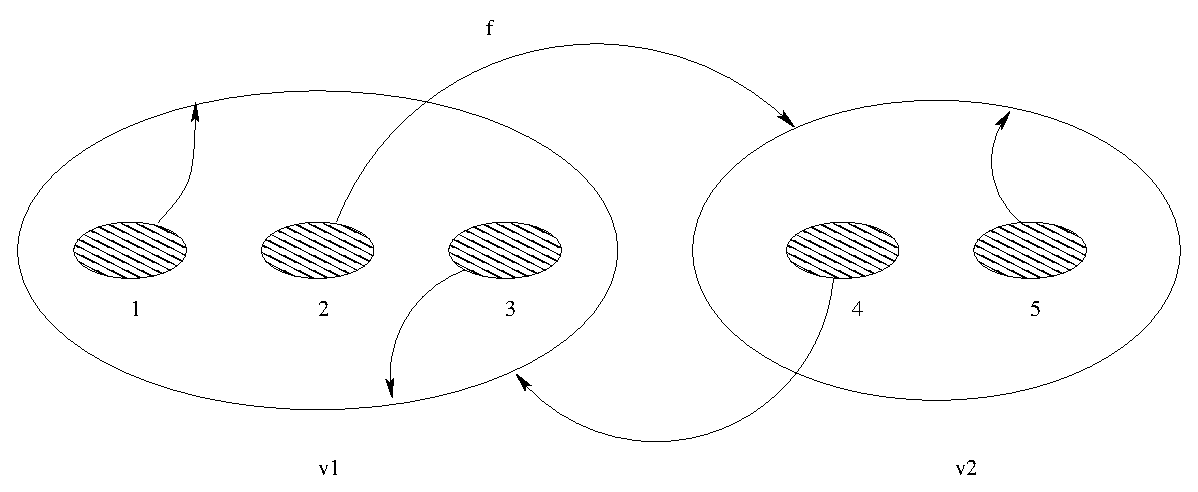
\includegraphics[scale=0.55]{cantor1.eps}
    \caption{A Cantor repeller. Figure captions will be flush-left
       and unjustified}
    \label{cantor}
\rule[-20pt]{\textwidth}{0.5pt}
\normalsize
\begin{verbatim}
  \begin{figure}
    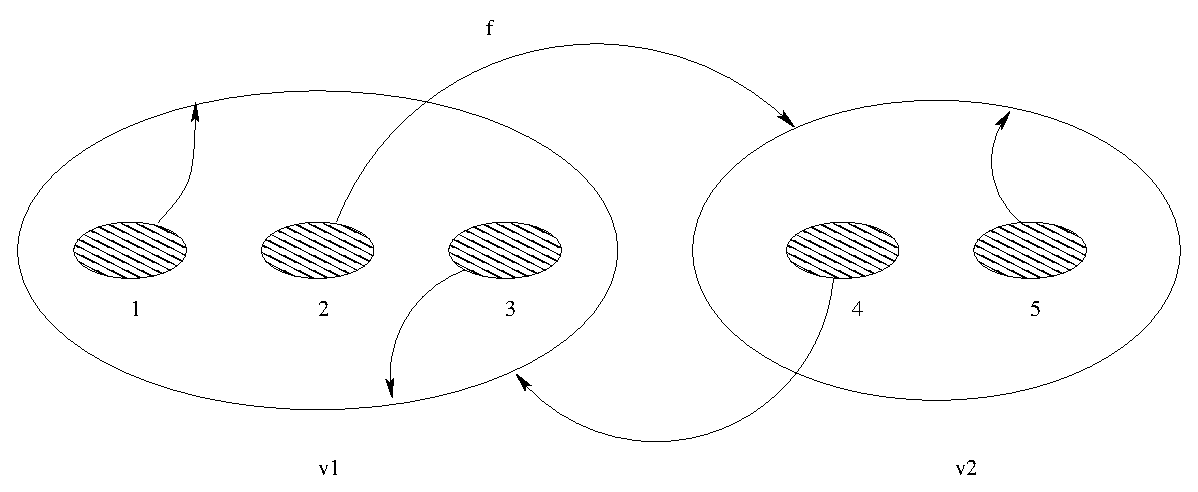
\includegraphics[scale=0.55]{cantor1.eps}
    \caption{A Cantor repeller. Figure captions will be flush-left
       and unjustified}
    \label{cantor}
  \end{figure}
\end{verbatim}
\rule[20pt]{\textwidth}{0.5pt}
  \end{figure}

\subsection{Wide figures 28--35pc}

Figures may extend the full width of the page, as illustrated in Figure~\ref{anothercantor}. To achieve this, you must add \verb"\widefigure" before inserting the artwork (see the source code immediately below this figure).
  \begin{figure}% code for wide figures
    \widefigure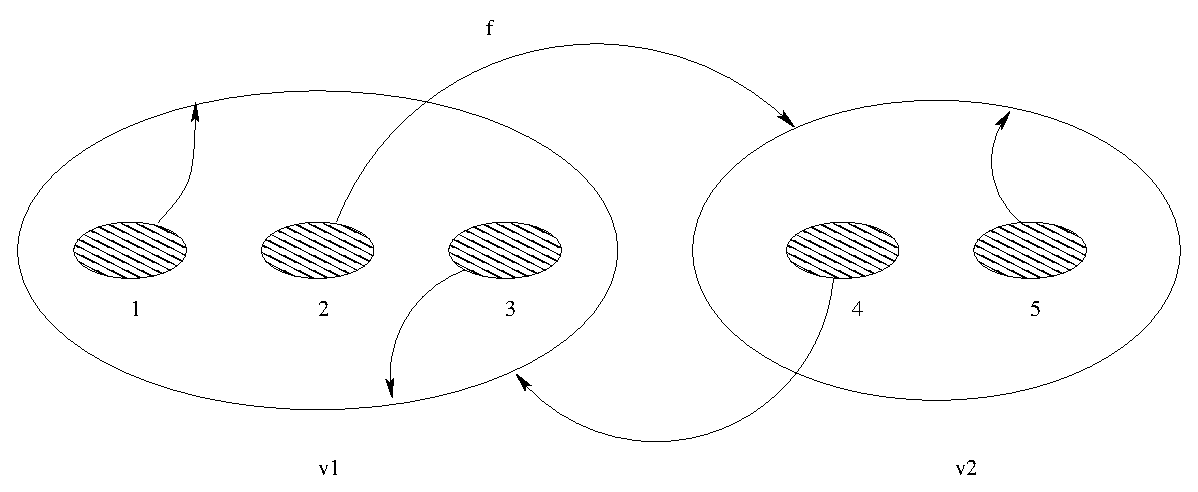
\includegraphics[width=35pc]{cantor1.eps}
    \caption{A~wide figure}
    \label{anothercantor}
  \rule[-20pt]{\textwidth}{0.5pt}
\normalsize
\begin{verbatim}
  \begin{figure}% code for wide figures
    \widefigure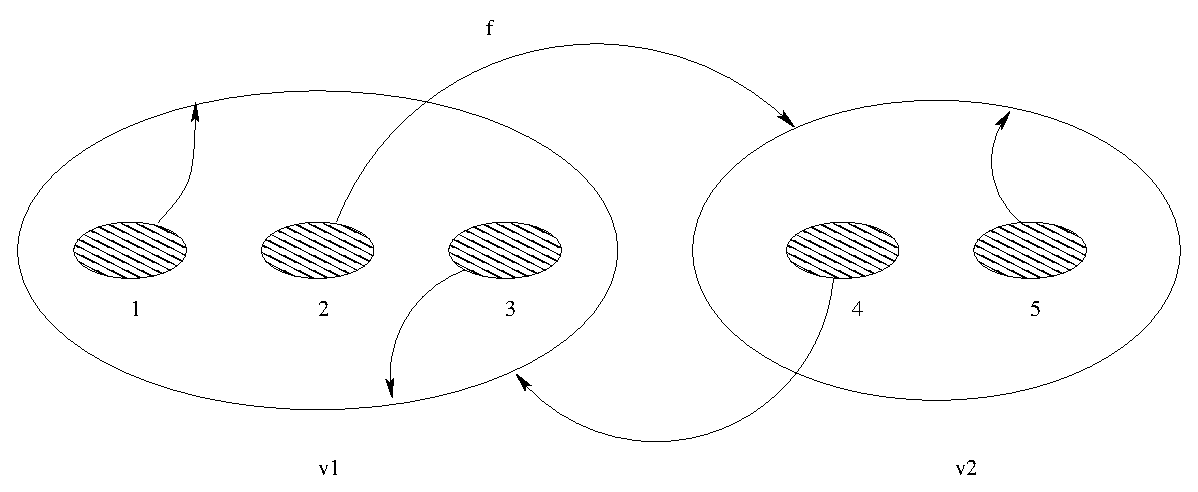
\includegraphics[width=35pc]{cantor1.eps}
    \caption{A~wide figure}
    \label{anothercantor}
  \end{figure}
\end{verbatim}
  \rule[20pt]{\textwidth}{0.5pt}
  \end{figure}

\section{Tables}
\label{tables}

Due to the complex specification for tables in the \cambridge\ design, they need to be typeset slightly differently. Please refer to the source code immediately below Table~\ref{sample-table}, where you will find the following construction:
\begin{verbatim}
  \begin{table}
    \processtable
    {Table caption\label{transformation}}
    {\begin{tabular}...\end{tabular}}
  \end{table}
\end{verbatim}
In other words, they are typeset using \verb"\processtable" which contains 2~arguments.

The \cambridge\ class will cope with most positioning of your tables. Table captions must be included first, the the label, then the body of the table.

  \begin{table}
    \processtable
    {Note that table captions are typeset using~the \texttt{processtable}
      macro\label{sample-table}}
    {\addtolength\tabcolsep{2pt}% to stretch columns, if required
      \begin{tabular}{c@{\hspace{25pt}}ccc}
        Figure\footnote{\textit{Note:} All generalizations are false,
        including this one.} & $hA$ & $hB$ & $hC$\\
        \hline
        1 & $\exp\left(\pi i\frac58\right)$
          & $\exp\left(\pi i\frac18\right)$ & $0$\\[3pt]
        2 & $-1$    & $\exp\left(\pi i\frac34\right)$ & $1$\\[12pt]
        3 & $-4+3i$ & $-4+3i$ & $\frac74$\\[3pt]
        4 & $-2$    & $-2$    & $\frac54 i$\\
        \hline
      \end{tabular}}
  \rule[-20pt]{\textwidth}{0.5pt}
\begin{verbatim}
  \begin{table}
    \processtable
    {Note that table captions are typeset using~the \texttt{processtable}
      macro\label{sample-table}}
    {\addtolength\tabcolsep{2pt}% to stretch columns, if required
      \begin{tabular}{c@{\hspace{25pt}}ccc}
        Figure\footnote{\textit{Note:} All generalizations are false,
        including this one.} & $hA$ & $hB$ & $hC$\\
        \hline
        1 & $\exp\left(\pi i\frac58\right)$
          & $\exp\left(\pi i\frac18\right)$ & $0$\\[3pt]
        2 & $-1$    & $\exp\left(\pi i\frac34\right)$ & $1$\\[12pt]
        3 & $-4+3i$ & $-4+3i$ & $\frac74$\\[3pt]
        4 & $-2$    & $-2$    & $\frac54 i$\\
        \hline
      \end{tabular}}
  \end{table}
\end{verbatim}
  \rule[20pt]{\textwidth}{0.5pt}
  \end{table}


\subsection{My vertical rules have disappeared}

Vertical rules in tables are not \cambridge\ style, and have been automatically removed; this gives your document a truly professional look. Instead of vertical rules, we recommend the use of extra horizontal space, see Section~\ref{addhoriz}. The rules have been removed by redefining the \verb"tabular" environment. The amended definition also inserts extra vertical space above and below the horizontal rules (produced by \verb"\hline").



If you really must have them reinstated, read Section~\ref{reinstate}.

\subsection{Reinstating the vertical rules}
\label{reinstate}
Authors can revert to the standard \LaTeX\ style, if necessary. Tables will take on a rather squashed appearance, as in the \LaTeX\ book, whereby there is no added space around horizontal rules. Add the command \verb"\reinstaterules" in the preamble, and re-run your files through \LaTeX.

\subsection{There is very little space around the rules in my~table}
Tables revert to the standard, rather squashed look of standard \LaTeX\ tables for two reasons:
\begin{enumerate}
  \item you are using \verb"array.sty"; or
  \item you have chosen to reinstate vertical rules (see Section~\ref{reinstate})
\end{enumerate}
In both cases, the tabular environment is redefined.


\subsection{Adding space between columns}
\label{addhoriz}
You can add space (2pt in this example) between every column using\linebreak \verb"\addtolength\tabcolsep{2pt}". However, if you only wanted to expand the space between columns~1 and~2 to~25pt, you would do this using\linebreak \verb"\begin{tabular}{@{}c@{\hspace{25pt}}ccc@{}}" (see Table~\ref{sample-table}).

\subsection{Adding space between rows}
If you need some form of separation between rows (for example, between rows~2 and~3 in the body of Table~\ref{sample-table}), adding \verb"[12pt]" immediately after the double backslash at the end of row~2 will add a 12pt vertical space (the equivalent of a blank line at this typesize). This is neater than adding another horizontal line.


\section{Landscape figures and tables, using rotating.sty}

Landscape figures and tables (floats) may be typeset using the \verb"rotating.sty" package. Note that the direction of rotation is always anti-clockwise, regardless of whether the rotated float lands on an even or odd page. To achieve this, be sure to add the optional argument \verb"[figuresright]" when calling in \verb"rotating.sty" (see below).

In addition to \verb"rotating.sty", you should also include \verb"floatpag.sty" and the command \verb"\rotfloatpagestyle{empty}". This combination ensures that headers and footers are removed from the float page:
\begin{verbatim}
  \usepackage[figuresright]{rotating}
  \usepackage{floatpag}
  \rotfloatpagestyle{empty}
\end{verbatim}
In some DVI previewers, floats may not appear rotated. If this happens, you need to convert the DVI file to PostScript or PDF.

Occasionally, when you convert a PostScript file to a PDF file, you may find that the page comes out upside-down. There will be a setting to change this. For instance, if you are using PDFCreator 0.9.7, choose the following options in this sequence:
\begin{description}
  \item Options -- Program -- PDF -- Auto-Rotate Pages: Change to `None'.
\end{description}
Other programs will have similar procedures.

\subsection{Coding for landscape figures}

The landscape figure (Figure~\ref{sidecantor}) was typeset using the following coding:
\begin{verbatim}
  \begin{sidewaysfigure}
    \centering
    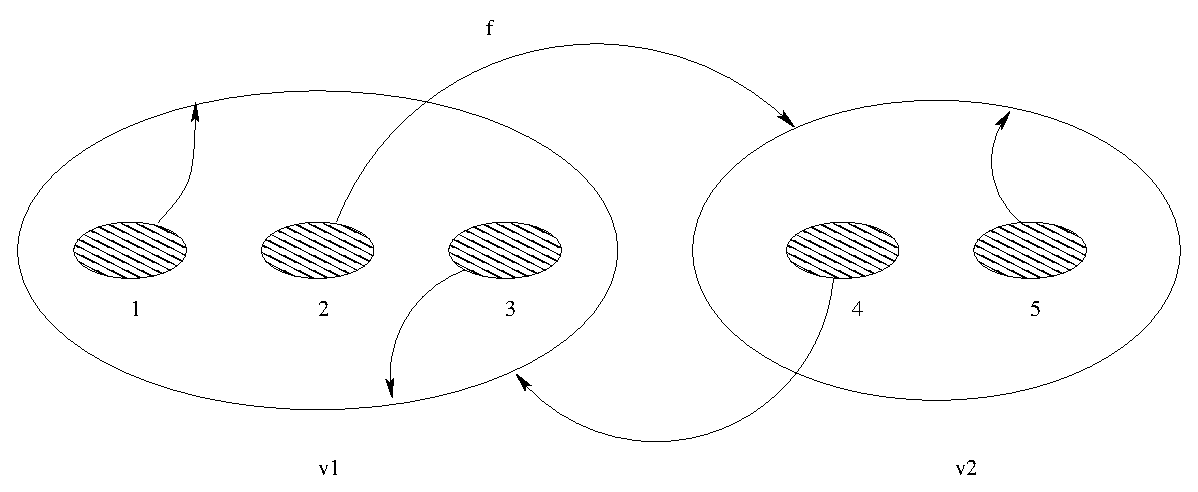
\includegraphics[scale=0.85]{cantor1.eps}
    \caption[Landscape figure]{A Cantor repeller. Figure captions
       will be flush-left and unjustified}
    \label{sidecantor}
  \end{sidewaysfigure}
\end{verbatim}
  \begin{sidewaysfigure}
    \centering
    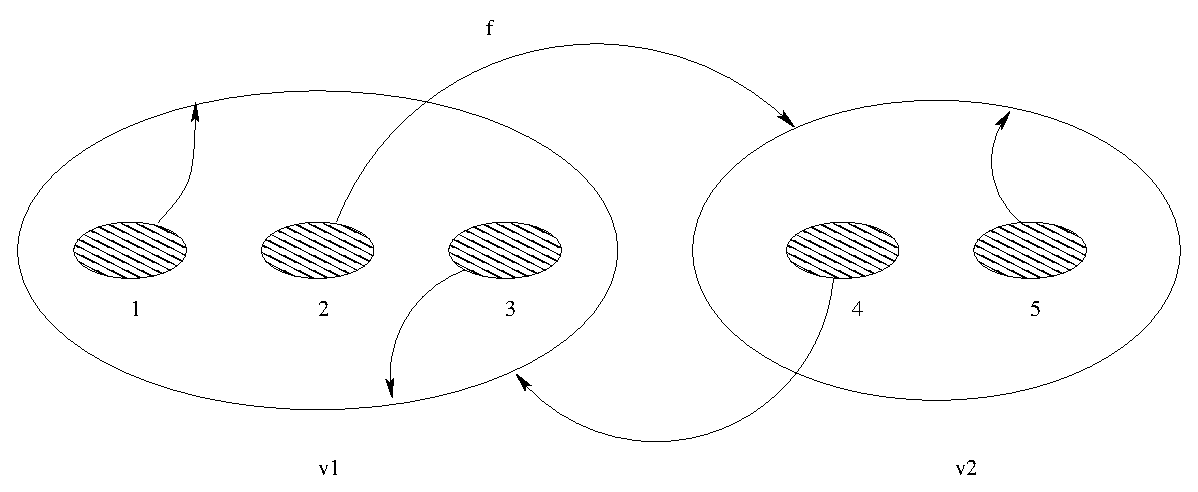
\includegraphics[scale=0.85]{cantor1.eps}
    \caption[Landscape figure]{A Cantor repeller. Figure captions
       will be flush-left and unjustified}
    \label{sidecantor}
  \end{sidewaysfigure}

\subsection{Coding for landscape tables}

Table~\ref{sideways} has been produced using the following coding:
%
\begin{smallverbatim}
\begin{sidewaystable}
  \processtable
  {Grooved ware and beaker features, their finds and
    radiocarbon dates. For a breakdown of the pottery assemblages see
    Tables~I and~III; for the flints see Tables~II and~IV; for the animal
    bones see Table~V.\label{sideways}}
  {\addtolength\tabcolsep{-2pt}
    \begin{tabular}{lcccllccccc}
    Context & Length & Breadth/  & Depth & Profile & Pottery & Flint & Animal
                                                     & Stone & Other & C14 Dates\\
    && Diameter &&&&& Bones\\[6pt]
    & m & m & m\\
    \hline\\[-5pt]
    \multicolumn{10}{l}{\textbf{Grooved Ware}}\\
    784 & --   & 0.9$\phantom{0}$ &0.18  & Sloping U & P1      & $\times$46
          & $\phantom{0}$$\times$8 && $\times$2 bone & 2150 $\pm$100\,\textsc{bc}\\
    785 & --   & 1.00             &0.12   & Sloping U & P2--4  & $\times$23
                                             & $\times$21 & Hammerstone & -- & --\\
    962 & --   & 1.37             &0.20   & Sloping U & P5--6  & $\times$48
                       & $\times$57 & --& --& 1990 $\pm$80\,\textsc{bc} (Layer 4)\\
    &&&&&&&&&& 1870 $\pm$90\,\textsc{bc} (Layer 1)\\
    983 & 0.83 & 0.73             &0.25   & Stepped U & --     & $\times$18
                                  & $\phantom{0}$$\times$8 & -- & Fired clay & --\\
    &&&&&&&&&&\\
    \multicolumn{10}{l}{\textbf{Beaker}}\\
    552 & --   & 0.68             & 0.12  & Saucer    & P7--14 & --           & --
                                                                     & -- &-- &--\\
    790 & --   & 0.60             & 0.25  & U         & P15    & $\times$12   & --
                                                        & Quartzite-lump & -- &--\\
    794 & 2.89 & 0.75             & 0.25  & Irreg.    & P16    & $\phantom{0}$$\times$3
                                                                & -- & -- &-- &--\\
    \end{tabular}}
\end{sidewaystable}
\end{smallverbatim}

\begin{sidewaystable}
  \processtable
  {Grooved ware and beaker features, their finds and
    radiocarbon dates. For a breakdown of the pottery assemblages see
    Tables~I and~III; for the flints see Tables~II and~IV; for the animal
    bones see Table~V.\label{sideways}}
  {\addtolength\tabcolsep{-2pt}
    \begin{tabular}{lcccllccccc}
    Context & Length & Breadth/  & Depth & Profile & Pottery & Flint & Animal
                                                     & Stone & Other & C14 Dates\\
    && Diameter &&&&& Bones\\[6pt]
    & m & m & m\\
    \hline\\[-5pt]
    \multicolumn{10}{l}{\textbf{Grooved Ware}}\\
    784 & --   & 0.9$\phantom{0}$ &0.18  & Sloping U & P1      & $\times$46
          & $\phantom{0}$$\times$8 && $\times$2 bone & 2150 $\pm$100\,\textsc{bc}\\
    785 & --   & 1.00             &0.12   & Sloping U & P2--4  & $\times$23
                                             & $\times$21 & Hammerstone & -- & --\\
    962 & --   & 1.37             &0.20   & Sloping U & P5--6  & $\times$48
                       & $\times$57 & --& --& 1990 $\pm$80\,\textsc{bc} (Layer 4)\\
    &&&&&&&&&& 1870 $\pm$90\,\textsc{bc} (Layer 1)\\
    983 & 0.83 & 0.73             &0.25   & Stepped U & --     & $\times$18
                                  & $\phantom{0}$$\times$8 & -- & Fired clay & --\\
    &&&&&&&&&&\\
    \multicolumn{10}{l}{\textbf{Beaker}}\\
    552 & --   & 0.68             & 0.12  & Saucer    & P7--14 & --           & --
                                                                     & -- &-- &--\\
    790 & --   & 0.60             & 0.25  & U         & P15    & $\times$12   & --
                                                        & Quartzite-lump & -- &--\\
    794 & 2.89 & 0.75             & 0.25  & Irreg.    & P16    & $\phantom{0}$$\times$3
                                                                & -- & -- &-- &--\\
    \end{tabular}}
\end{sidewaystable}

  \begin{summary}
    A summary may be added at the end of each chapter using the
    coding below. The heading is a numbered section head; the text
    is slightly larger and sans-serif.
  \end{summary}
\begin{verbatim}
  \begin{summary}
    A summary may be added at the end of each chapter using the
    coding below. The heading is a numbered section head; the text
    is slightly larger and sans-serif.
  \end{summary}
\end{verbatim}
\endinput

% features of the \cambridge\ class file
  % chap3.tex
% 2010/12/03, v1.20

\chapter{Mathematical solutions}
\label{mathsol}

\section{Why are we using amsthm.sty?}

Many authors are already using this style file, so we have decided that rather than re-invent the wheel, we will make it part of our distribution. This means that the top of the root file would include the following lines:\\[0.5\baselineskip]
\verb"  \documentclass{"\texttt{\cambridge}\verb"}"\\
\verb"    :"\\
\verb"  \usepackage{amsmath}"\\
\verb"  \usepackage{amsthm}"\\[0.5\baselineskip]
As mentioned in Chapter~\ref{intro}, if your book does not use theorems, proofs, etc., then there is no need to include the amsthm package, but you do need to include these files to run this guide through \LaTeX. Note that if you are also using \verb"amsmath.sty", it \emph{must} precede \verb"amsthm.sty".

The instructions for amsthm.sty are documentated separately in \texttt{amsthdoc.pdf}. We are including \texttt{amsthm.sty} and \texttt{amsthdoc.pdf} in this distribution for your convenience, but you may find more recent versions on the web. The following sections discuss the basic features, plus a few extras.

To save time, you may cut and paste the code in Appendix~\ref{amsthmcommands} into your root file. This is a comprehensive (but not necessarily a complete) list of theorem-like environments you may wish to use.

The \verb"amsthm" commands used in this guide are detailed in Appendix~\ref{rootfile}. They are simply a subset of commands from Appendix~\ref{amsthmcommands}; some illustrate unnumbered versions.

Please note that theorems, definitions, remarks, etc.\ should be numbered in a single sequence, either by chapter (Chapter~4 would have Definition~4.1, Lemma~4.2, Lemma~4.3, Proposition~4.4, Corollary~4.5) or by section (Definition~4.1.1, Lemma~4.1.2, Lemma~4.1.3, Proposition~4.1.4, Corollary~4.1.5).

To number these elements by chapter in this guide, we have used\linebreak \verb"\newtheorem{theorem}{Theorem}[chapter]". If you prefer to have the elements numbered by section, replace \verb"[chapter]" with \verb"[section]".

\section{amsthm styles}

If no \verb"\theoremstyle" command is given, the style used will be \texttt{plain}. To specify different styles, divide your \verb"\newtheorem" commands into groups and preface each group with the appropriate \verb"\theoremstyle".

\subsection{amsthm \texttt{plain} style}

The \texttt{plain} style is normally used for theorems, lemmas, corollaries, propositions, conjectures, criterion and algorithms. Authors are free to define their preferred numbering systems for these. The following example resets the theorem numbers for each chapter; lemmas follow in the same sequence. We have also requested that corollaries remain unnumbered by using the starred version:
\begin{verbatim}
  \theoremstyle{plain}% default
  \newtheorem{theorem}{Theorem}[chapter]
  \newtheorem{lemma}[theorem]{Lemma}
  \newtheorem*{corollary}{Corollary}

  \begin{theorem}
    Let the scalar function\ldots
  \end{theorem}
  \begin{lemma}[Tranah]
    The first-order free surface amplitudes\ldots
  \end{lemma}
  \begin{lemma}[\citealp{MenshEst}]
    The exotic behaviours of Lagrangian\ldots
  \end{lemma}
  \begin{corollary}
    Let $G$ be the free group on\ldots
  \end{corollary}
\end{verbatim}
will produce the following output:
  \begin{theorem}
    Let the scalar function\ldots
  \end{theorem}
  \begin{lemma}[Tranah]
    The first-order free surface amplitudes\ldots
  \end{lemma}
  \begin{lemma}[\citealp{MenshEst}]
    The exotic behaviours of Lagrangian\ldots
  \end{lemma}
  \begin{corollary}
    Let $G$ be the free group on\ldots
  \end{corollary}
%
Note that Corollaries would normally be in the same numbering sequence as Theorems and Lemmas. If you'd prefer your theorems to be typeset in roman (though this is not recommended) use the amsthm \texttt{definition} style instead (see Section~\ref{amsdefn}).

\subsection{amsthm \texttt{definition} style}
\label{amsdefn}

The \texttt{definition} style is normally used for definitions and conditions. Again, authors are free to define their preferred numbering systems for these. However, it is most usual to continue with the same numbering sequence as for Theorems, Lemmas, etc.:
\begin{verbatim}
  \theoremstyle{definition}
  \newtheorem{definition}[theorem]{Definition}
  \newtheorem{condition}[theorem]{Condition}

  \begin{definition}
    The series above is the Green function\ldots
  \end{definition}
  \begin{definition}
    The correlation between the real and estimated flow\ldots
  \end{definition}
  \begin{condition}
    The length (i.e. number of letters) of a word $w\in [s]^*$\ldots
  \end{condition}
\end{verbatim}
will produce the following output:
  \begin{definition}
    The series above is the Green function\ldots
  \end{definition}
  \begin{definition}
    The correlation between the real and estimated flow\ldots
  \end{definition}
  \begin{condition}
    The length (i.e. number of letters) of a word $w\in [s]^*$\ldots
  \end{condition}

\subsection{amsthm \texttt{remark} style}

The \texttt{remark} style is normally used for remarks, notes, notation, claims, summary, acknowledgements, cases, conclusions. However, in the \cambridge\ design, the remark and definition styles are the same. Authors who have already used the \texttt{remark} style may continue to do so; authors who are just starting out may choose to continue to use the \texttt{definition} style for remarks, notes, etc. Authors are free to define their preferred numbering systems for these.
\begin{verbatim}
  \theoremstyle{remark}
  \newtheorem*{remark}{Remark}
  \newtheorem*{case}{Case}

  \begin{remark}
    The absolute amplitude of a stratified wake\ldots
  \end{remark}
  \begin{case}
    The profiles of quadratic fluctuations\ldots
  \end{case}
\end{verbatim}
will produce the following output:
  \begin{remark}
    The absolute amplitude of a stratified wake\ldots
  \end{remark}
  \begin{case}
    The profiles of quadratic fluctuations\ldots
  \end{case}

\section{Proofs}
\label{proofs}

The \verb"proof" environment is also part of the amsthm package, and provides a consistent format for proofs.
 For example,
\begin{verbatim}
  \begin{proof}
    Use $K_\lambda$ and $S_\lambda$ to translate combinators
    into $\lambda$-terms. For the converse, translate
    $\lambda x$ \ldots by [$x$] \ldots and use induction
    and the lemma.
  \end{proof}
\end{verbatim}
produces the following:
  \begin{proof}
    Use $K_\lambda$ and $S_\lambda$ to translate combinators
    into $\lambda$-terms. For the converse, translate
    $\lambda x$ \ldots by [$x$] \ldots and use induction
    and the lemma.
  \end{proof}

\subsection{Changing the word `Proof' to something else}

An optional argument allows you to substitute a different name for the standard `Proof'. To change the proof heading to read `Proof of the Pythagorean Theorem', key the following:
\begin{verbatim}
  \begin{proof}[Proof of the Pythagorean Theorem]
    Start with a generic right-angled triangle\ldots
  \end{proof}
\end{verbatim}
which produces:
  \begin{proof}[Proof of the Pythagorean Theorem]
    Start with a generic right-angled triangle\ldots
  \end{proof}


\subsection{Typesetting a proof without a \hbox{\qedsymbol}}

This is not part of the amsthm package. Use the \verb"proof*" version. For example,
\begin{verbatim}
  \begin{proof*}
    The apparent virtual mass coefficient\ldots
  \end{proof*}
\end{verbatim}
produces the following:
  \begin{proof*}
    The apparent virtual mass coefficient\ldots
  \end{proof*}

\subsection{Placing the \hbox{\qedsymbol} after a displayed equation}

To avoid the \qedsymbol\ dropping onto the following line at the end of a proof,
\begin{verbatim}
  \begin{proof}
    \ldots and, as we are all aware,
    \[
       E=mc^2. \qedhere
    \]
  \end{proof}
\end{verbatim}
produces the following:
  \begin{proof}
    \ldots and, as we are all aware,
    \[
       E=mc^2. \qedhere
    \]
  \end{proof}
When used with the amsmath package, version~2 or later, \verb"\qedhere" will position \qedsymbol\ flush right; with earlier versions, \qedsymbol\ will be spaced a quad away
from the end of the text or display.

If \verb"\qedhere" produces an error message in an equation, try using \verb"\mbox{\qedhere}" instead.

\subsection{Placing the \hbox{\qedsymbol} after a displayed eqnarray}

This is also not part of the amsthm package. To enable this, you need to used the starred version of \verb"proof", and add both \verb"\arrayqed" and \verb"\arrayqedhere", as shown in the following example:
\begin{verbatim}
  \begin{proof*}
    The following equations prove the theorem:
      \arrayqed
        \begin{eqnarray}
          \epsilon &=& -\frac{1}{2}U_0\frac{\mathrm{d}q'^2}
                       {\mathrm{d}x}\nonumber\\
                   &=& 10\nu\frac{q'^2}{\lambda^2}
        \arrayqedhere
        \end{eqnarray}
  \end{proof*}
\end{verbatim}
produces the following:
  \begin{proof*}
    The following equations prove the theorem:
      \arrayqed
        \begin{eqnarray}
          \epsilon &=& -\frac{1}{2}U_0\frac{\mathrm{d}q'^2}
                       {\mathrm{d}x}\nonumber\\
                   &=& 10\nu\frac{q'^2}{\lambda^2}
        \arrayqedhere
        \end{eqnarray}
  \end{proof*}

\section{Boxed equations}

Important equations may be highlighted using the \verb"shadedbox" environment. You would not normally include text in such a box, but it is included here to demonstrate how to add a footnote. Euler might have included the following equation in his thesis:
  \begin{shadedbox}
    This is one way\footnotemark\ to define $e$:
    \begin{equation}
      e = \lim_{n\to\infty} \left( 1 + \frac{1}{n} \right)^n
    \end{equation}
  \end{shadedbox}
  \footnotetext{There are others.}
\begin{samepage}
\noindent Here is the code for the above:
\begin{verbatim}
  \begin{shadedbox}
    This is one way\footnotemark\ to define $e$:
    \begin{equation}
      e = \lim_{n\to\infty} \left( 1 + \frac{1}{n} \right)^n
    \end{equation}
  \end{shadedbox}
  \footnotetext{There are others.}
\end{verbatim}
\end{samepage}
\endinput
% mathematical solutions

  \part{Closing features}
  % chap4.tex
% 2010/12/03, v1.20

\chapter{Reference and bibliography lists}

\section{Automatic lists using Bib\TeXinsectionhead}

We have chosen to use the natbib package because of its versatility.

First, call in \texttt{natbib.sty}. If you are using the multi-contributor option, you will get an unnumbered section heading, otherwise it will be an unnumbered chapter heading.

The bibliography file for this guide (\texttt{\cambridge guide.tex}) is called \texttt{percolation.bib}; the bibliography style is \texttt{cambridgeauthordate.bst}, so place the final two commands at the point where you would like the references to appear:
%
\begin{verbatim}
    \usepackage{natbib}
      :
  % \renewcommand{\refname}{Bibliography}
    \bibliography{percolation}
    \bibliographystyle{cambridgeauthordate}
\end{verbatim}
%
Note that if you uncomment the third line shown above, you can change the heading from `References' to `Bibliography'. Next, \LaTeX\ your book twice. Then run \textsc{Bib}\TeX\ by executing the command\\[0.5\baselineskip]
\verb"  bibtex "\texttt{\cambridge guide}\\[0.5\baselineskip]
Finally, run your book through \LaTeX\ twice again. This series of runs will generate a file called \texttt{\cambridge guide.bbl}, which will then be included by \verb"\bibliography{percolation}".

Suppose you have cited 8 entries from the `percolation' database, e.g. \verb"\citealp{MenshEst}"; \verb"\citealp{Kasymp}"; \verb"\citealp{VGFH}"; \verb"\citealp{HamMaz94}"; \verb"\citealp{HamLower}"; \verb"\citealp{AiBar87}"; \verb"\citealp{MMS}"; and \verb"\citealp{HamAtomBond}"; the output will be just those 8~entries (see page~\pageref{refs}).%
% add these entries to the list without referring to them
\nocite{MenshEst}\nocite{Kasymp}\nocite{VGFH}\nocite{HamMaz94}\nocite{HamLower}\nocite{AiBar87}\nocite{MMS}\nocite{HamAtomBond}

\section{Citations using natbib commands}
Here are some of the basic citation commands available with the natbib package; there are many more if you cannot find what you need in this list. Bear in mind that Menshikov (1985) or (Menshikov, 1985) read best, depending on context.\\*[0.5\baselineskip]
\begin{tabular}{@{}ll@{}}
\verb"\citep{MenshEst}"
    & $\rightarrow\enskip$\citep{MenshEst}\\
\verb"\citep[see][p.$\,$34]{MenshEst}"
    & $\rightarrow\enskip$\citep[see][p.$\,$34]{MenshEst}\\
\verb"\citep[e.g.][]{MenshEst}"
    & $\rightarrow\enskip$\citep[e.g.][]{MenshEst}\\
\verb"\citep[Section~2.3]{MenshEst}"
    & $\rightarrow\enskip$\citep[Section~2.3]{MenshEst}\\
\verb"\citep{MenshEst, VGFH}"\\
    & $\hspace{-70pt}\rightarrow\enskip$\citep{MenshEst, VGFH}\\
\verb"\cite{MenshEst, VGFH}"\\
    & $\hspace{-70pt}\rightarrow\enskip$\cite{MenshEst, VGFH}\\
\verb"\citealt{MenshEst}"
    & $\rightarrow\enskip$\citealt{MenshEst}\\
\verb"\cite{MenshEst}"
    & $\rightarrow\enskip$\cite{MenshEst}\\
\verb"\citealp{MenshEst}"
    & $\rightarrow\enskip$\citealp{MenshEst}\\
\verb"\citeauthor{MenshEst}"
    & $\rightarrow\enskip$\citeauthor{MenshEst}\\
\verb"\citeyearpar{MenshEst}"
    & $\rightarrow\enskip$\citeyearpar{MenshEst}\\
\verb"\citeyear{MenshEst}"
    & $\rightarrow\enskip$\citeyear{MenshEst}
\end{tabular}


\section{How to change reference entries from author--date to~numbers}
\label{numberedbiblio}

\LaTeX\ authors are used to \verb"\cite{...}" producing a reference such as~[11] in their manuscripts. If you prefer this style, it is an option within the natbib package:
\begin{verbatim}
  \usepackage[numbers]{natbib}
\end{verbatim}

\section{Keying in your reference list for an author--date system}
\label{authordatebiblio}

The entries need to be keyed as below. Note that if you uncomment the first line, you can change the heading from `References' to `Bibliography':
%
\begin{smallverbatim}
% \renewcommand{\refname}{Bibliography}
  \begin{thebibliography}{8}
    \expandafter\ifx\csname natexlab\endcsname\relax
      \def\natexlab#1{#1}\fi
    \expandafter\ifx\csname selectlanguage\endcsname\relax
      \def\selectlanguage#1{\relax}\fi

  \bibitem[Aizenman and Barsky, 1987]{AiBar87}
    Aizenman, M., and Barsky, D.~J. 1987.
    Sharpness of the phase transition in percolation models.
    {\em Comm. Math. Phys.}, {\bf 108}, 489--526.

  \bibitem[Hammersley, 1957]{HamLower}
    Hammersley, J.~M. 1957.
    Percolation processes: Lower bounds for the critical probability.
    {\em Ann. Math. Statist.}, {\bf 28}, 790--795.

  \bibitem[Hammersley, 1961]{HamAtomBond}
    Hammersley, J.~M. 1961.
    Comparison of atom and bond percolation processes.
    {\em J. Mathematical Phys.}, {\bf 2}, 728--733.

  \bibitem[Hammersley and Mazzarino, 1994]{HamMaz94}
    Hammersley, J.~M., and Mazzarino, G. 1994.
    Properties of large Eden clusters in the plane.
    {\em Combin. Probab. Comput.}, {\bf 3}, 471--505.

  \bibitem[Kesten, 1990]{Kasymp}
    Kesten, H. 1990.
    Asymptotics in high dimensions for percolation.
    Pages  219--240 of: Grimmett, G.~R., and Welsh, D.~J.~A. (eds),
    {\em Disorder in Physical Systems: A Volume in Honour of John Hammersley}.
    Oxford University Press.

  \bibitem[Menshikov, 1985]{MenshEst}
    Menshikov, M.~V. 1985.
    Estimates for percolation thresholds for lattices in {${\bf R}\sp n$}.
    {\em Dokl. Akad. Nauk SSSR}, {\bf 284}, 36--39.

  \bibitem[Menshikov et~al., 1986]{MMS}
    Menshikov, M.~V., Molchanov, S.~A., and Sidorenko, A.~F. 1986.
    Percolation theory and some applications.
    Pages  53--110 of: {\em Probability theory. Mathematical
    statistics. Theoretical cybernetics, Vol. 24 (Russian)}.
    Akad. Nauk SSSR Vsesoyuz. Inst. Nauchn. i Tekhn. Inform.
    Translated in {\em J. Soviet Math}. {\bf 42} (1988), no. 4,
    1766--1810.

  \bibitem[Vyssotsky et~al., 1961]{VGFH}
    Vyssotsky, V.~A., Gordon, S.~B., Frisch, H.~L., and Hammersley, J.~M. 1961.
    Critical percolation probabilities (bond problem).
    {\em Phys. Rev.}, {\bf 123}, 1566--1567.

  \end{thebibliography}
\end{smallverbatim}

\section{Keying in your reference list for a numbered system}

For this style, you may omit the optional square brace shown in Section~\ref{authordatebiblio}. Once again, if you uncomment the first line, you can change the heading from `References' to `Bibliography':
%
\begin{smallverbatim}
% \renewcommand{\refname}{Bibliography}
  \begin{thebibliography}{8}

  \bibitem{AiBar87}
    Aizenman, M., and Barsky, D.~J. 1987.
    Sharpness of the phase transition in percolation models.
    {\em Comm. Math. Phys.}, {\bf 108}, 489--526.

  \bibitem{HamLower}
    Hammersley, J.~M. 1957.
    Percolation processes: Lower bounds for the critical probability.
    {\em Ann. Math. Statist.}, {\bf 28}, 790--795.

  \bibitem{HamAtomBond}
    Hammersley, J.~M. 1961.
    Comparison of atom and bond percolation processes.
    {\em J. Mathematical Phys.}, {\bf 2}, 728--733.
      :
      :
  \bibitem[Vyssotsky et~al., 1961]{VGFH}
    Vyssotsky, V.~A., Gordon, S.~B., Frisch, H.~L., and Hammersley, J.~M. 1961.
    Critical percolation probabilities (bond problem).
    {\em Phys. Rev.}, {\bf 123}, 1566--1567.

  \end{thebibliography}
\end{smallverbatim}

\endinput% references and bibliographies
  % chap5.tex
% 2010/12/03, v1.20

\chapter{Indexes}
\label{indexes}

\section{Creating a single index using makeidx.sty}
To generate a single index, normally a subject index, the commands would take the form:
\begin{verbatim}
  \index{diffraction}
  \index{force!hydrodynamic}
  \index{force!interactive}
\end{verbatim}
  %\index{diffraction}%
  %\index{force!hydrodynamic}%
  %\index{force!interactive}%
The following commands are then required in the preamble:
\begin{verbatim}
  \usepackage{makeidx}
  \makeindex
\end{verbatim}
and at the point you wish your index to appear,
\begin{verbatim}
  \printindex
\end{verbatim}
Run your book through \LaTeX\ enough times so that the labels, etc., are stable. Then execute the command:\\[0.5\baselineskip]
\verb"  makeindex "\texttt{\cambridge guide}\\[0.5\baselineskip]
To include the index, you need to run \LaTeX\ one more time.


\section{Creating multiple indexes using multind.sty}
This guide has been prepared using \verb"multind.sty". This style file redefines the \verb"\makeindex", \verb"\index" and \verb"\printindex" commands to deal with multiple indexes.

Suppose you want to create an author index and a subject index. The entries should be in the text as usual, but take the following form:
\begin{verbatim}
  \index{authors}{Young, P.D.F.}
  \index{authors}{Tranah, D.A.}
  \index{authors}{Peterson, K.}
  \index{subject}{diffraction}
  \index{subject}{force!hydrodynamic}
  \index{subject}{force!interactive}
\end{verbatim}
  \index{authors}{Young, P.D.F.}%
  \index{authors}{Tranah, D.A.}%
  \index{authors}{Peterson, K.}%
  \index{subject}{diffraction}%
  \index{subject}{force!hydrodynamic}%
  \index{subject}{force!interactive}%
In the preamble, you need to add the following lines:
\begin{verbatim}
  \usepackage{multind}\ProvidesPackage{multind}
  \makeindex{authors}
  \makeindex{subject}
\end{verbatim}
It is crucial to add the command \verb"\ProvidesPackage{multind}"; this will send a message to the class file to re-style the index into the \cambridge\ style. You will get a warning in your log file:
\begin{verbatim}
  LaTeX Warning: You have requested package `',
                 but the package provides `multind'.
\end{verbatim}
which can be ignored. At the point where you wish your indexes to appear, you then need the commands:
\begin{verbatim}
  \printindex{authors}{Author index}
  \printindex{subject}{Subject index}
\end{verbatim}
Run your book through \LaTeX\ enough times so that the labels, etc., are stable. Then execute the commands:
\begin{verbatim}
  makeindex authors
  makeindex subject
\end{verbatim}
To include the indexes, you need to run \LaTeX\ one more time.

\section{Creating multiple indexes using index.sty}

This style file allows you to define new indexes. Suppose you want to create an author index as well as a normal subject index. The entries should be in the text as usual, but take the following form:
\begin{verbatim}
  \index[aut]{Young, P.D.F.}
  \index[aut]{Tranah, D.A.}
  \index[aut]{Peterson, K.}
  \index{diffraction}
  \index{force!hydrodynamic}
  \index{force!interactive}
\end{verbatim}
  %\index[aut]{Young, P.D.F.}%
  %\index[aut]{Tranah, D.A.}%
  %\index[aut]{Peterson, K.}
  %\index{diffraction}%
  %\index{force!hydrodynamic}%
  %\index{force!interactive}%
To create the extra author index, you need to have the following lines in the preamble:
\begin{verbatim}
  \usepackage{index}
  \newindex{aut}{adx}{and}{Author index}
  \makeindex
\end{verbatim}
At the point where you wish your indexes to appear, use:
\begin{verbatim}
  \printindex[aut]
  \printindex
\end{verbatim}
Run your book through \LaTeX\ enough times so that the labels, etc., are stable. Then execute the commands:\\[0.5\baselineskip]
\verb"  makeindex -o "\texttt{\cambridge guide.and \cambridge guide.adx}\\
\verb"  makeindex "\texttt{\cambridge guide}\\[0.5\baselineskip]
To include the indexes, you need to run \LaTeX\ one more time.

\subsection{Caution -- from the authors of index.sty}

In order to implement \verb"index.sty", it's been necessary to modify a number of \LaTeX\ commands seemingly unrelated to indexing, namely, \verb"\@starttoc", \verb"\raggedbottom", \verb"\flushbottom", \verb"\addcontents", \verb"\markboth", and \verb"\markright". Naturally, this could cause incompatibilities between \texttt{index.sty} and any style files that either redefine these same commands or make specific assumptions about how they operate.

The redefinition of \verb"\@starttoc" is particularly bad, since it introduces an incompatibility with the AMS document classes. This will be addressed soon.

In the current implementation, \texttt{index.sty} uses one output stream for each index.  Since there are a limited number of output indexes, this means that there is a limit on the number of indexes you can have in a document.  There is more information on this in \verb"index.dtx" which is part of the \verb"index.sty" distribution.\\[\baselineskip]
%
\textit{For these reasons, whilst all care has been taken to deal with these changes in \cambridge.cls, if you do find incompatibilities with other files, please contact us at texline@cambridge.org with your source files, class and style files, and log file.}

\endinput
% single and multiple indexes

  \backmatter
% if you only have one appendix, use \oneappendix instead of \appendix

  \appendix
  % appendixA.tex
% 2010/12/03, v1.20

\chapter{Typesetting appendices}

\section{Single-contributor books}
\subsection{How to typeset one appendix}
If you have just one appendix, say \verb"appendix.tex", you will want to generate a chapter head `Appendix' rather than `Appendix A'. Use \verb"\oneappendix" in the main file, as follows:
\begin{verbatim}
  \oneappendix
  \include{appendix}
\end{verbatim}

\subsection{How to typeset several appendices}
The coding used to generate the appendices in this guide is as follows:
\begin{verbatim}
  \appendix
  \include{appendixA}
  \include{appendixB}
  \include{appendixC}
\end{verbatim}

\section{Multi-contributor books}

\subsection{How to typeset one appendix}
If you have just one appendix, it will be the next section head and you should include the following code at the end of your chapter:
\begin{verbatim}
  \oneappendix
  \section{Appendix heading}
  \subsection{Subheading}
  \endappendix
\end{verbatim}
You will need to add \verb"\endappendix" if you have further section heads in this chapter.


\subsection{How to typeset several appendices}
The following code will genenerate Appendix~A and Appendix~B at the end of your chapter:
\begin{verbatim}
  \appendix
  \section{Appendix heading}
  \subsection{Subheading}
    :
  \section{Next appendix heading}
  \subsection{Next subheading}
  \endappendix
\end{verbatim}
Again, you will need to add \verb"\endappendix" if you have further section heads in this chapter.

\section{Numbering systems}

Equations in appendices will be numbered as follows:
\begin{equation}
  E=mc^2,
\end{equation}
and figure captions as follows:
\begin{figure}[h]
\caption{Similarity solutions}
\end{figure}

\endinput
  % appendixB.tex
% 2010/12/03, v1.20

\chapter{amsthm commands}
\label{amsthmcommands}

The following code may be cut and pasted into your root file. Assuming you have included \verb"amsthm.sty", it will number your theorems, definitions, etc. in the same numbering sequence and by chapter, e.g.~Definition~4.1, Lemma~4.2, Lemma~4.3, Proposition~4.4, Corollary~4.5.

If you prefer to have the elements numbered by section, e.g.~Definition~4.1.1, Lemma~4.1.2, Lemma~4.1.3, Proposition~4.1.4, Corollary~4.1.5, replace \verb"[chapter]" on line 2 with \verb"[section]".

\begin{smallverbatim}

  \theoremstyle{plain}% default
  \newtheorem{theorem}{Theorem}[chapter]
  \newtheorem{lemma}[theorem]{Lemma}
  \newtheorem{corollary}[theorem]{Corollary}
  \newtheorem{proposition}[theorem]{Proposition}
  \newtheorem{conjecture}[theorem]{Conjecture}
  \newtheorem{criterion}[theorem]{Criterion}
  \newtheorem{algorithm}[theorem]{Algorithm}

  \theoremstyle{definition}
  \newtheorem{definition}[theorem]{Definition}
  \newtheorem{condition}[theorem]{Condition}

  \theoremstyle{remark}
  \newtheorem{remark}[theorem]{Remark}
  \newtheorem{note}[theorem]{Note}
  \newtheorem{notation}[theorem]{Notation}
  \newtheorem{claim}[theorem]{Claim}
  \newtheorem{summary}[theorem]{Summary}
  \newtheorem{acknowledgement}[theorem]{Acknowledgement}
  \newtheorem{case}[theorem]{Case}
  \newtheorem{conclusion}[theorem]{Conclusion}
\end{smallverbatim}

\endinput
  % appendixC.tex
% 2010/12/03, v1.20

\chapter{The root file for this~guide}
\label{rootfile}

\vfill
\begin{smallverbatim}
% PT3guide.tex
% for the suite of standard Cambridge designs
% 2010/12/03, v1.20

  \NeedsTeXFormat{LaTeX2e}[1996/06/01]

% \documentclass[multi]{PT3}  % multi-contributor option
% \documentclass[prodtf]{PT3} % production option (used to produce PT3guide.pdf);
                              % can only be used if you have the Adobe Myriad Pro
                              % Condensed font
  \documentclass{PT3}
  \usepackage{tikz}           % coding for topic boxes
                              %   (also calls in graphicx.sty)
  \usepackage{natbib}
  \usepackage[figuresright]{rotating}
  \usepackage{floatpag}
    \rotfloatpagestyle{empty}

% \usepackage{amsmath}        % if you are using this package,
                              % it must be loaded before amsthm.sty
  \usepackage{amsthm}

% \usepackage{txfonts}        % times font (used to produce PT3guide.pdf)

% indexes
% uncomment the relevant set of commands

% for a single index
% \usepackage{makeidx}
% \makeindex

% for multiple indexes using multind.sty
  \usepackage{multind}\ProvidesPackage{multind}
  \makeindex{authors}
  \makeindex{subject}

% for multiple indexes using index.sty
% \usepackage{index}
% \newindex{aut}{adx}{and}{Author index}
% \makeindex

  \newcommand\cambridge{PT3}

% see chapter 3 for details
  \theoremstyle{plain}% default
  \newtheorem{theorem}{Theorem}[chapter]
  \newtheorem{lemma}[theorem]{Lemma}
  \newtheorem*{corollary}{Corollary}

  \theoremstyle{definition}
  \newtheorem{definition}[theorem]{Definition}
  \newtheorem{condition}[theorem]{Condition}
  \newtheorem{example-norules}[theorem]{Example}%

  \theoremstyle{remark}
  \newtheorem*{remark}{Remark}
  \newtheorem*{case}{Case}

  \hyphenation{line-break line-breaks docu-ment triangle cambridge
    amsthdoc cambridgemods baseline-skip author authors
    cambridgestyle en-vir-on-ment polar astron-omers solu-tion}

  \setcounter{tocdepth}{2}    % the toc normally lists sections; for the purposes of
                              % this document, this has been extended to subsections

%%%%%%%%%%%%%%%%%%%%%%%%%%%%%%%%%%%%%

% \includeonly{chap2}

%%%%%%%%%%%%%%%%%%%%%%%%%%%%%%%%%%%%%

  \begin{document}

  \title[Subtitle, If You Have One]
    {\LaTeXeintitle\ Guide for Authors using~the~\cambridge~Design}

  \author{Ali Woollatt}

  \details{This guide was compiled using \cambridge.cls \version\\[\baselineskip]
    The latest version can be downloaded from:
    https://authornet.cambridge.org/information/productionguide/
      LaTeX\_files/\cambridge.zip}

  \frontmatter
  \maketitle
  \tableofcontents
  \listoffigures
  \listoftables
  \listoffloatingboxes
  \listofcontributors

  \mainmatter
  \partquote{I have called this principle, by which each slight variation,
    if useful, is preserved, by the term of Natural Selection.}{Charles Darwin}
    \label{partquote}
  \part{Getting started}
  \include{chap1}% introduction
  \include{chap2}% features of the \cambridge\ class file
  \include{chap3}% mathematical solutions

  \part{Closing features}
  \include{chap4}% references and bibliographies
  \include{chap5}% single and multiple indexes

  \backmatter
% if you only have one appendix, use \oneappendix instead of \appendix

  \appendix
  \include{appendixA}
  \include{appendixB}
  \include{appendixC}
  \endappendix

% insert a blank line to the toc list
  \addtocontents{toc}{\vspace{\baselineskip}}
  \theendnotes

% \renewcommand{\refname}{Bibliography}% if you prefer this heading
  \bibliography{percolation}\label{refs}
  \bibliographystyle{cambridgeauthordate}

  \cleardoublepage

% indexes

% for a single index
% \printindex

% for multiple indexes using multind.sty
  \printindex{authors}{Author index}
  \printindex{subject}{Subject index}

% for multiple indexes using index.sty
% \printindex[aut]
% \printindex

\end{document}
\end{smallverbatim}
\endinput
  \endappendix

% insert a blank line to the toc list
  \addtocontents{toc}{\vspace{\baselineskip}}
  \theendnotes

% \renewcommand{\refname}{Bibliography}% if you prefer this heading
  \bibliography{percolation}\label{refs}
  \bibliographystyle{cambridgeauthordate}

  \cleardoublepage

% indexes

% for a single index
% \printindex

% for multiple indexes using multind.sty
  \printindex{authors}{Author index}
  \printindex{subject}{Subject index}

% for multiple indexes using index.sty
% \printindex[aut]
% \printindex

\end{document}
\end{smallverbatim}
\endinput
\end{verbatim}

\section{Multi-contributor books}

\subsection{How to typeset one appendix}
If you have just one appendix, it will be the next section head and you should include the following code at the end of your chapter:
\begin{verbatim}
  \oneappendix
  \section{Appendix heading}
  \subsection{Subheading}
  \endappendix
\end{verbatim}
You will need to add \verb"\endappendix" if you have further section heads in this chapter.


\subsection{How to typeset several appendices}
The following code will genenerate Appendix~A and Appendix~B at the end of your chapter:
\begin{verbatim}
  \appendix
  \section{Appendix heading}
  \subsection{Subheading}
    :
  \section{Next appendix heading}
  \subsection{Next subheading}
  \endappendix
\end{verbatim}
Again, you will need to add \verb"\endappendix" if you have further section heads in this chapter.

\section{Numbering systems}

Equations in appendices will be numbered as follows:
\begin{equation}
  E=mc^2,
\end{equation}
and figure captions as follows:
\begin{figure}[h]
\caption{Similarity solutions}
\end{figure}

\endinput
\chapter{\text{Acyclic models and model categories}}
\section{Acyclic models theorem}
In algebraic topology, the acyclic models theorem can be used to show that two homology theories are isomorphic and usually applying it would great simplify the proof. It can be thought of as a ``universal pattern'' of homology theories.
\begin{definition}Let $\calc$ be a category.
A family of \textbf{models} in $\calc$ is simply an indexed subset $\pzm=\{M_\lambda|\lambda\in \Lambda\}$ of $obj(\calc)$.
\end{definition}

\begin{definition}
Let $\calc$ be a category with family of models $\pzm=\{M_\lambda|\lambda\in \Lambda\}$.  Suppose $T:\calc\lrta Ab$ is a functor. A $T$-\textbf{model set} $\chi$ is a choice of elements $x_\lambda\in T(M_\lambda)$ for each $\lambda$:
$$
\chi=\{x_\lambda\in T(M_\lambda)|\lambda\in \Lambda\}
$$
\end{definition}

\begin{definition}
Let $\calc$ be a category with family of models $\pzm=\{M_\lambda|\lambda\in \Lambda\}$. Suppose $T:\calc\lrta Ab$ is a functor. We say that $T$ is \textbf{free with basis in} $\pzm$ if the following condition holds:
\begin{enumerate}
\item $T(C)$ is a free abelian group $\forall C\in \calc$
\item There is a $T$-model set $\chi=\{x_\lambda\in T(M_\lambda)|\lambda\in \Lambda\}$ s.t.
$$
\{T(f)(x_\lambda)|f\in \hom(M_\lambda,C), \lambda\in \Lambda\}
$$
is a basis for the free abelian group $T(C)$.
\end{enumerate}
We call $\chi$ a \textbf{model basis} for $T$.
\end{definition}
We say $T_\bullet:\calc\lrta Comp$ if free with basis in $\pzm$ if each $T_n$ is free with basis in $\pzm$.

\begin{definition}
$T_\bullet:\calc\lrta Comp$, we say $T_\bullet$ is \textbf{non-negative} if $T_n(C)=0$ for all $n<0$ and $\forall C$. $T_\bullet$ is \textbf{acyclic in the positive degrees on $C$} or $C$ \textbf{is $T_\bullet$-acyclic } if $H_n(T_\bullet(C))=0,\forall n>0$. 
\end{definition}

\begin{example}
Take $\calc=Top$, $\pzm=\{\Delta^n|n\geq 0\}$.  $T_\bullet$ is the singular chain functor.
$$
\calc_\bullet: Top\lrta Comp
$$
$$
X\mapsto C_\bullet(X)
$$
By definition, $T_\bullet$ is free with basis in $\pzm$.
Then $T_\bullet$ is non-negative because
$C_\bullet$ is non-negative, \checkmark. Also, $\Delta^n$ is $T_\bullet$-acyclic
$H_n(C_\bullet(\Delta^i))=H_n(\Delta^i)=0,\forall n>0$\checkmark. (We say $\pzm$ is $T_\bullet$-acyclic)
\end{example}
\begin{theorem}\label{apendix:thm:Acyclic_models_theorem}
Suppose $\calc$ is a category with models $\pzm$. Suppose $T_\bullet, S_\bullet:\calc\lrta Comp$ are two functors such that both $T_\bullet$ and $S_\bullet$ are non-negative. Assume further $T_\bullet$ is free with basis in $\pzm$ and $S_\bullet$ is acyclic in the positive degree on each element $M\in\pzm$.

Suppose 
$$
\Theta: H_0\circ T_\bullet\lrta H_0\circ S_\bullet
$$
 is a natural transformation. $\exists $ a  natural chain morphism $\Psi_\bullet:T_\bullet\lrta S_\bullet$ which is unique up to natural chain homotopy and has $H_0(\Psi_\bullet)=\Theta$.
\end{theorem}
\begin{corollary}
We will be mostly interested in the case where both $S_\bullet$ and $T_\bullet$ are free with basis $\pzm$ and that each model $M\in\pzm$ is both $S_\bullet$-acyclic and $T_\bullet$-acyclic. In this case if $\Theta: H_0\circ T_\bullet\lrta H_0\circ S_\bullet$ is a natural equivalence then every natural chain map $\Phi_\bullet$ inducing $\Theta$ is natural chain equivalence.
\end{corollary}
\begin{corollary}\label{appendixAcor:chain_homotopy_over_H0(f)_free_acyclic}
Suppose $(C_\bullet, \pd)$ and $(D_\bullet, \pd')$ are two non-negative chain complexes. Assume $C_\bullet$ is free and that $D_\bullet$ is acyclic in positive degrees. Then given any homomorphism $h: H_0(C_\bullet)\lrta H_0(D_\bullet)$, there exists a chain map $f_\bullet: C_\bullet\lrta D_\bullet$ over $h$ and this chain map is unique up to chain homotopy.

Moreover, if both non-negative chain complexes $C_\bullet$ and $D_\bullet$ are free and acyclic, and $h: H_0(C_\bullet)\lrta H_0(D_\bullet)$ is an isomorphism, then the chain map $g_\bullet$ is a chain equivalence.
\end{corollary}
Both corollaries can be directly derived, the first from the definition of chain equivalence and in the second, we choose the category with only one object.


To prove Theorem~\ref{apendix:thm:Acyclic_models_theorem}, we need to first quote some two lemmas
\begin{lemma}\label{apendixA:lem:A.1.3}
Let $\calc$ be a category with family of models $\pzm=\{M_\lambda|\lambda\in \Lambda\}$. Assume $S,T:\calc\lrta Ab$ are functors and assume $T$ is free with basis in $\pzm$. Let
$\chi:=\{x_\lambda\in T(M_\lambda)|\lambda\in \Lambda\}$ denote the model basis for $T$. Choose element $y_\lambda\in S(M_\lambda)$ for each $\lambda\in \Lambda$, and set $\Upsilon:=\{y_\lambda\in S(M_\lambda)|\lambda\in\Lambda\}$. Then there exists a unique natural transformation $\Phi:T\lrta S$ such that 
$$
\Phi(M_\lambda)(x_\lambda)=y_\lambda,\forall \lambda\in \Lambda
$$
\end{lemma}
\begin{proof}
Because $T$ is free with basis $\pzm$, we know for each $C\in\calc$, $T(C)$ is free abelian group and
$$
\{T(f)(x_\lambda)|f\in \hom(M_\lambda,C), \lambda\in \Lambda\}
$$
is a basis for the free abelian group $T(C)$. For fixed $\lambda\in \Lambda$ and fixed object $C\in obj(\calc)$, we have a commutative diagram for every morphism $f: M_\lambda\lrta C$
\[
\begin{tikzcd}
T(M_\lambda) \arrow[r, "T(f)"] \arrow[d, "\Phi(M_\lambda)"'] & T(C) \arrow[d, "\Phi(C)"] \\
S(M_\lambda) \arrow[r, "S(f)"'] & S(C)
\end{tikzcd}
\]
We have $\Phi(C)\circ T(f)(x_\lambda)=S(f)(y_\lambda)$. Since $T(f)(x_\lambda)$ forms a basis of $T(C)$, we know $\Phi(C)$ is uniquely determined, therefore $\Phi$ is unique if it exists.

It indeed exists. Fix any object $C\in \calc$, then by assumption $\{T(f)(x_\lambda)\}$ form a basis of $T(C)$ and $\Phi(C)(T(f)(x_\lambda))=S(f)(x_\lambda)$ by the universal property of free abelian group, there exists a unique homomorphism $\Phi(C):T(C)\lrta S(C)$ that restricts to it on basis. 

We have proved each individual $\Phi(C)$ exists and is unique. It only lefts to check that such specified $\Phi$ is indeed a natural transformation
\[
\begin{tikzcd}
T(A) \arrow[r, "T(g)"] \arrow[d, "\Phi(A)"'] & T(B) \arrow[d, "\Phi(B)"] \\
S(A) \arrow[r, "S(g)"'] & S(B)
\end{tikzcd}
\]
Given a typical basis element $T(f)(x_\lambda)$ for some $\lambda\in \Lambda$ and $f\in \hom(M_\lambda,A)$. Then 
$$
S(g)\circ \Phi(A)(T(f)(x_\lambda))=S(g)S(f)y_\lambda=S(g\circ f) y_\lambda.
$$
But also going the other way round:
$$
\Phi(B)\circ T(g) (T(f)(x_\lambda))=\Phi(B)(Tg\circ f)(x_\lambda)=S(g\circ f)(x_\lambda).
$$
Thus  $\Phi$ is indeed a natural transformation.
\end{proof}
\begin{lemma}\label{appendixA:lem:A.1.4}
Let $\calc$ be category with family of models $\pzm$. Suppose given six functors
$T_i,S_i:\calc\lrta Ab$, $i=0,1,2$. together with six natural transformations as pictured below
\[
\begin{tikzcd}
T_2 \arrow[r, "\Phi_2"] & T_1 \arrow[r, "\Phi_1"] \arrow[d, "\Theta_1"] & T_0 \arrow[d, "\Theta_0"] \\
S_2 \arrow[r, "\Psi_2"'] & S_1 \arrow[r, "\Psi_1"'] & S_0
\end{tikzcd}
\]
Assume that 
\begin{enumerate}
	\item For every object $C\in obj(\calc)$, the composition $\Phi_1(C)\circ \Phi_2(C):T_2(C)\lrta T_0(C)$ is the zero homomorphism.
	\item The bottom row is exact on $\pzm$, in the sense that for every model $M\in\pzm$, one has $\im \Psi_2(M)=\ker \Psi_1(M)$.
	\item The diagram commutes for every object $C\in obj(\calc)$.
	\item $T_2$ is free with basis in $M$.
\end{enumerate}
Then there exists a natural transformation $\Gamma:T_2\lrta S_2$ such the the first square commutes for every object of $\calc$.
\[
\begin{tikzcd}
T_2\ar[d, dashed, "\Gamma"] \arrow[r, "\Phi_2"] & T_1 \arrow[r, "\Phi_1"] \arrow[d, "\Theta_1"] & T_0 \arrow[d, "\Theta_0"] \\
S_2 \arrow[r, "\Psi_2"'] & S_1 \arrow[r, "\Psi_1"'] & S_0
\end{tikzcd}
\]
\end{lemma}
\begin{proof}
Let $\chi=\{x_\lambda\in T_2(M_\lambda)|\lambda\in \Lambda\}$ denote a model basis for $T_2$. Then for each $\lambda\in \Lambda$ we have a commutative diagram in $Ab$ such that both top row and bottom row are chain complex and the bottom row is exact. Also $T_2(M_\lambda)$ is free 
\[
\begin{tikzcd}
T_2(M_\lambda)\ar[d, dashed, "\gamma"] \arrow[r, "f_2"] & T_1(M_\lambda) \arrow[r, "f_1"] \arrow[d, "t_1"] & T_0(M_\lambda) \arrow[d, "t_0"] \\
S_2(M_\lambda) \arrow[r, "g_2"'] & S_1(M_\lambda) \arrow[r, "g_1"'] & S_0(M_\lambda)
\end{tikzcd}
\]
$\im t_1\circ f_2\subset \im g_2$ because $g_1\circ t_1\circ f_2=h\circ f_1\circ f_2=0$, hence $\im t_1\circ f_2\subset \ker g_1=\im g_2$. For each $x_\lambda$, there is a $y_\lambda\in S_2(M_\lambda)$ such that $g_2(y_\lambda)=t_1\circ f_2(x_\lambda)$ because $g_2$ is surjective. By universal property of free module, we get a unique morphism $\gamma:T_2(M_\lambda)\lrta S_2(M_\lambda)$ such that $\gamma(x_\lambda)=y_\lambda$. (But because $y_\lambda$ are not unique, $\gamma$ is not the unique morphism that makes the triangle commute)
\[
\begin{tikzcd}
 & T_2(M_\lambda) \arrow[d, "t_1\circ f_2"] \arrow[ld, "\exists \gamma"', dashed] &  \\
S_2(M_\lambda) \arrow[r, "g_2"] & \im g_2 \arrow[r] & 0.
\end{tikzcd}
\]
(It also makes the first square of the previous diagram commutes).
We then know by~\ref{apendixA:lem:A.1.3} there exists a unique natural transformation $\Gamma: T_2\lrta S_2$ such that
$$
\Gamma(M_\lambda)(x_\lambda)=y_\lambda, \forall \lambda\in \Lambda.
$$ 

It remains to check thus constructed $\Gamma$ makes the functor diagram commutes. If we define $z_\lambda:=\Psi_2(M_\lambda)(y_\lambda)=\Theta_1(M_\lambda)(\Phi(M_\lambda)(x_\lambda))$, $\Theta_1\circ\Phi_2$ and $\Psi\circ \Gamma$ are two natural transformations that sends $x_\lambda$ to $z_\lambda$. Then we know the first square of functor diagram commutes by the uniqueness in~\ref{apendixA:lem:A.1.3}.
\end{proof}
Finally we come back to the proof of Theorem~\ref{apendix:thm:Acyclic_models_theorem}.
\begin{proof}{of theorem A.1.1}

1. \underline{Such $\Phi_\bullet$ exists}: 
We need to construct natural transformations $\Phi_n:S_n\lrta T_n$ such that the following diagram commutes.
\[\begin{tikzcd}
\cdots \arrow[r, "\pd"] & T_2 \arrow[r, "\pd"] \arrow[d, "\Phi_2", dashed] & T_1 \arrow[r, "\pd"] \arrow[d, "\Phi_1", dashed] & T_0 \arrow[r] \arrow[d, "\Phi_0", dashed] & H_0(T_\bullet) \arrow[r] \arrow[d, "\Theta"] & 0 \\
\cdots \arrow[r, "\pd'"] & S_2 \arrow[r, "\pd'"] & S_1 \arrow[r, "\pd'"] & S_0 \arrow[r] & H_0(S_\bullet) \arrow[r] & 0
\end{tikzcd}
\]
With Lemma~\ref{appendixA:lem:A.1.4} in hand, we can induct on $n$ to concatenate the ``ladders''.

For $n=0$, we have
\[
\begin{tikzcd}
T_0 \arrow[r] \arrow[d, "\exists \Phi_0"', dashed] & H_0(T_\bullet) \arrow[r] \arrow[d] & 0 \arrow[d] \\
S_0 \arrow[r] & H_0(S_\bullet) \arrow[r] & 0
\end{tikzcd}
\]
\end{proof}

If we find $\Phi_i, 0\leq i\leq n$ such that makes the first $n$ ladder commute, we can find a $\Phi_{n+1}$ that makes the diagram commute
\[
\begin{tikzcd}
T_{n+1} \arrow[r] \arrow[d, "\exists \Phi_{n+1}"', dashed] & T_n \arrow[r] \arrow[d, "\Phi_n"] & T_{n-1} \arrow[d, "\Phi_{n-1}"] \\
S_{n+1} \arrow[r] & S_n \arrow[r] & S_{n-1}
\end{tikzcd}
\]

2. \underline{$H_0(\Phi_\bullet)=\Theta$}: This is a direct result of the corresponding diagram of  chain complexes. On each object $C$, $H_0(\Phi_\bullet)(C): H_0(T_\bullet(C))\lrta H_0(S_\bullet(C)):\lgl c\rgl\mapsto \lgl \Phi_0(c)\rgl$
Then we have $H_0(\Phi_\bullet)(C)=\Theta(C)$ because the right most square commutes when applied to object $C$.

3. \underline{$\Phi_\bullet$ is unique up to natural chain homotopy} Suppose now we have two such maps $\Psi_\bullet,\Phi_\bullet: T_\bullet\lrta S_\bullet$. We need to find natural transformation $\Upsilon_n: T_{n}\lrta S_{n+1}$ for $n\geq -1$ such that 
$$
\pd'\Upsilon_n+\Upsilon_{n-1}\pd=\Phi_n-\Psi_n.
$$
Denote the difference $\Phi_n-\Psi_n=:\Xi_n$. We define $\Upsilon_{-1}=0$ and proceed inductively. We have a diagram
\[
\begin{tikzcd}
T_0 \arrow[r] \arrow[d, "\exists\Upsilon_0"', dashed] & T_0 \arrow[d, "\Xi_0"] \arrow[r] & 0 \arrow[d, "0"] \\
S_1 \arrow[r] & S_0 \arrow[r] & H_0(S_\bullet),
\end{tikzcd}
\]
where we have used~\ref{appendixA:lem:A.1.4} again. Inductively, If we have constructed $\Upsilon_{n-1}$, we have the following diagram
\[
\begin{tikzcd}
T_n \arrow[r, "id"] \arrow[d, "\exists \Upsilon_{n}"', dashed] & T_n \arrow[d, "\Xi_n-\Upsilon_{n-1}\circ\pd"] \arrow[r] & 0 \arrow[d, "0"] \\
S_{n+1} \arrow[r, "\pd'"] & S_n \arrow[r] & S_{n-1}
\end{tikzcd}
\] 
By induction hypothesis, the above diagram commutes because
$$
\begin{aligned}
\pd'(\Xi_n-\Upsilon_{n-1}\pd)\\
&=\pd'\Xi_n-\pd'\Upsilon_{n-1}\pd\\
&=\pd'\Xi_n-(\Xi_{n-1}-\Upsilon_{n-1}\pd)\pd\\
&=\pd'\Xi_n-\Xi_{n-1}\pd\\
&=0.
\end{aligned}
$$
Hence, we can construct $\Upsilon_{n}$ by~\ref{appendixA:lem:A.1.4}.





\section{Model categories}
Model categories catch the essence of homotopy. In order to study homotopic invariant, we need machinery to construct (weak) homotopy invariant functors.

\begin{definition}
A \textbf{model category} on a category $\calc$ consists of three distinguished classes of morphisms:\textbf{weak equivalences, fibrations} and \textbf{cofibrations} and two functorial factorizations $(\alpha,\beta)$ and $(\gamma,\delta)$ subject to the following axioms. Each classes of morphisms contain all the identities and are closed under composition of morphisms.
\begin{enumerate}[label=MC\arabic*:]
\item Finite limits and colimits exists in $\calc$
\item If $f,g$ are maps in $\calc$ such that $g\circ f$ is defined and if two of the three maps $f,g,g\circ f$ are weak equivalences, then so is the third.
\item If $f$ is a retract of $g$ and $g$ is a fibration, cofibration or weak equivalence, then so if $f$.
\item Given a commutative diagram of the 
\end{enumerate} 
\end{definition}

Similar with the localization of rings, we can inverse morphisms for some collection of morphisms.
\begin{definition}\textbf{Localization of a category}:
Given a category $\calc$ and some class $W$ of morphisms in $\calc$. (similar to localization of rings, we don't need $W$ to be multiplicatively closed, because the construction will naturally lead to multiplicative closure of $W$). We can define it by universal property: there is a natural localization functor $\calc\lrta W^{-1}\calc$ and given any other category $\mathcal{D}$, a functor $F:\calc\lrta\mathcal{D}$ factors uniquely through $\calc\lrta W^{-1}\calc$ iff $F$ sends every morphism in $W$ to an isomorphism in $\mathcal{D}$
\[
\begin{tikzcd}
\calc \arrow[d, "\iota_W"'] \arrow[r, "F"] & \mathcal{D} \\
W^{-1}\calc \arrow[ru, "\exists!"', dashed] & 
\end{tikzcd}
\]
\end{definition}

\chapter{Derived functors and derived categories}
\section{More on Tor and Ext}
%----------------------------------------------------------------------------------------
%	BIBLIOGRAPHY
%----------------------------------------------------------------------------------------

\chapter*{Bibliography}
\addcontentsline{toc}{chapter}{\textcolor{ocre}{Bibliography}}

%------------------------------------------------

\section*{Articles}
\addcontentsline{toc}{section}{Articles}
\printbibliography[heading=bibempty,type=article]

%------------------------------------------------

\section*{Books}
\addcontentsline{toc}{section}{Books}
\printbibliography[heading=bibempty,type=book]

%----------------------------------------------------------------------------------------
%	INDEX
%----------------------------------------------------------------------------------------

\cleardoublepage
\phantomsection
\setlength{\columnsep}{0.75cm}
\addcontentsline{toc}{chapter}{\textcolor{ocre}{Index}}
\printindex

%----------------------------------------------------------------------------------------

\end{document}
